% coding:utf-8

%----------------------------------------
%FOSAINKT, a LaTeX-Code for a summary of information and
%communication technology
%Copyright (C) 2015, Mario Felder & Michi Fallegger

%This program is free software; you can redistribute it and/or
%modify it under the terms of the GNU General Public License
%as published by the Free Software Foundation; either version 2
%of the License, or (at your option) any later version.

%This program is distributed in the hope that it will be useful,
%but WITHOUT ANY WARRANTY; without even the implied warranty of
%MERCHANTABILITY or FITNESS FOR A PARTICULAR PURPOSE.  See the
%GNU General Public License for more details.
%----------------------------------------

\documentclass[a5paper,10pt,fleqn]{book}

\usepackage{fosainkt_layout}

%\setboolean{ti}{true}        % Anleitung für TI-89

\title{Formelsammlung INKT}
% \ifti
% \title{Formelsammlung INKT \\ Mit Anleitung zu TI-89}
% \fi

\author{Mario Felder}
\date{\today}

%\catcode `\*=\active
%\def *{\cdot}

\begin{document}

\maketitle

\tableofcontents
% coding:utf-8

%----------------------------------------
%FOSAINKT, a LaTeX-Code for a summary of information and
%communication technology
%Copyright (C) 2015, Mario Felder & Michi Fallegger

%This program is free software; you can redistribute it and/or
%modify it under the terms of the GNU General Public License
%as published by the Free Software Foundation; either version 2
%of the License, or (at your option) any later version.

%This program is distributed in the hope that it will be useful,
%but WITHOUT ANY WARRANTY; without even the implied warranty of
%MERCHANTABILITY or FITNESS FOR A PARTICULAR PURPOSE.  See the
%GNU General Public License for more details.
%----------------------------------------
\chapter{Einleitung}
Energie:
\[
	E_s= \int_{0}^{T} \left|s(t)\right|^2 \di t
\]
~\\
Korrelation (Skalarprodukt):
\[
	\left\langle s_1,s_2 \right\rangle = \int_{0}^{T} s_1(t) \cdot s_2^*(t) \di t
\]
~\\
zwei Signale sind orthogonal wenn:
\[
	\left\langle s_1,s_2 \right\rangle = 0
\]
~\\
Amplitudenspektrum:
\[
	S(f) = \mathcal{F}\left\lbrace s(t) \right\rbrace = \int_{-\infty}^{\infty} s(t) \e^{-\im 2 \pi ft} \di t
\]
~\\
Parsevalsches Theorem:
\[
	\left\langle s_1,s_2 \right\rangle = \int_{-\infty}^{\infty} S_1(f) \cdot S_2^*(f) \di f
\]
~\\
Leistungsdichtespektrum $\Gamma_{ss}(f)$ (unter der Annahme, dass die Symbolfolge
mittelwertfrei, in der Leistung auf 1 normiert und unkorreliert ist):
\[
	\Gamma_{ss}(f) = \frac{1}{T_s} \left|P(f)\right|^2
\]
~\\
P-Norm:
\[
	\left||x\right||_p = \left(\sum_{i}\left|x_i\right|^p\right)^\frac{1}{p}
\]
\chapter{Basisband- und Bandpasssignale}
Spektrum von Basisbandsignal:
\begin{center}
	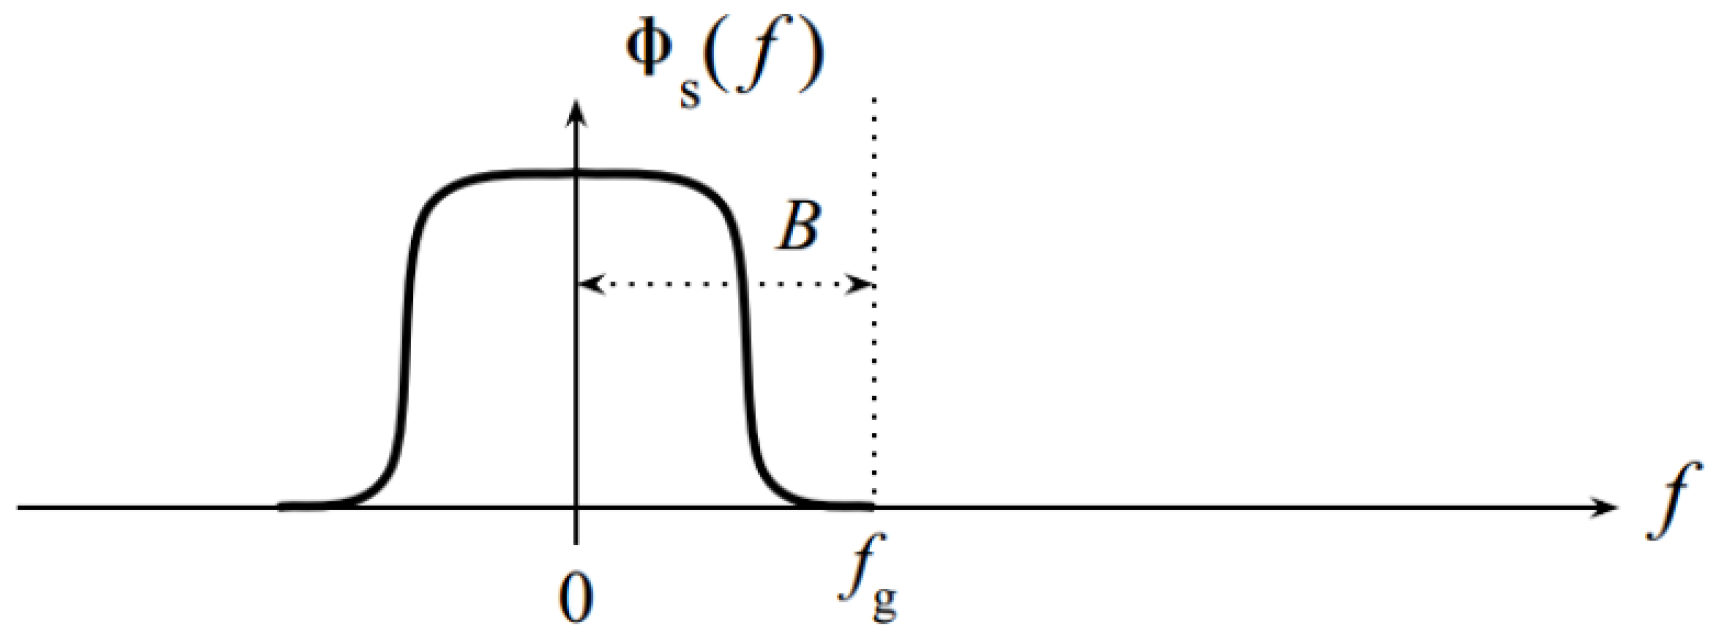
\includegraphics[width=0.8\textwidth]{./images/spek_basis}
\end{center}
~\\
Spektrum von Bandpasssignal
\begin{center}
	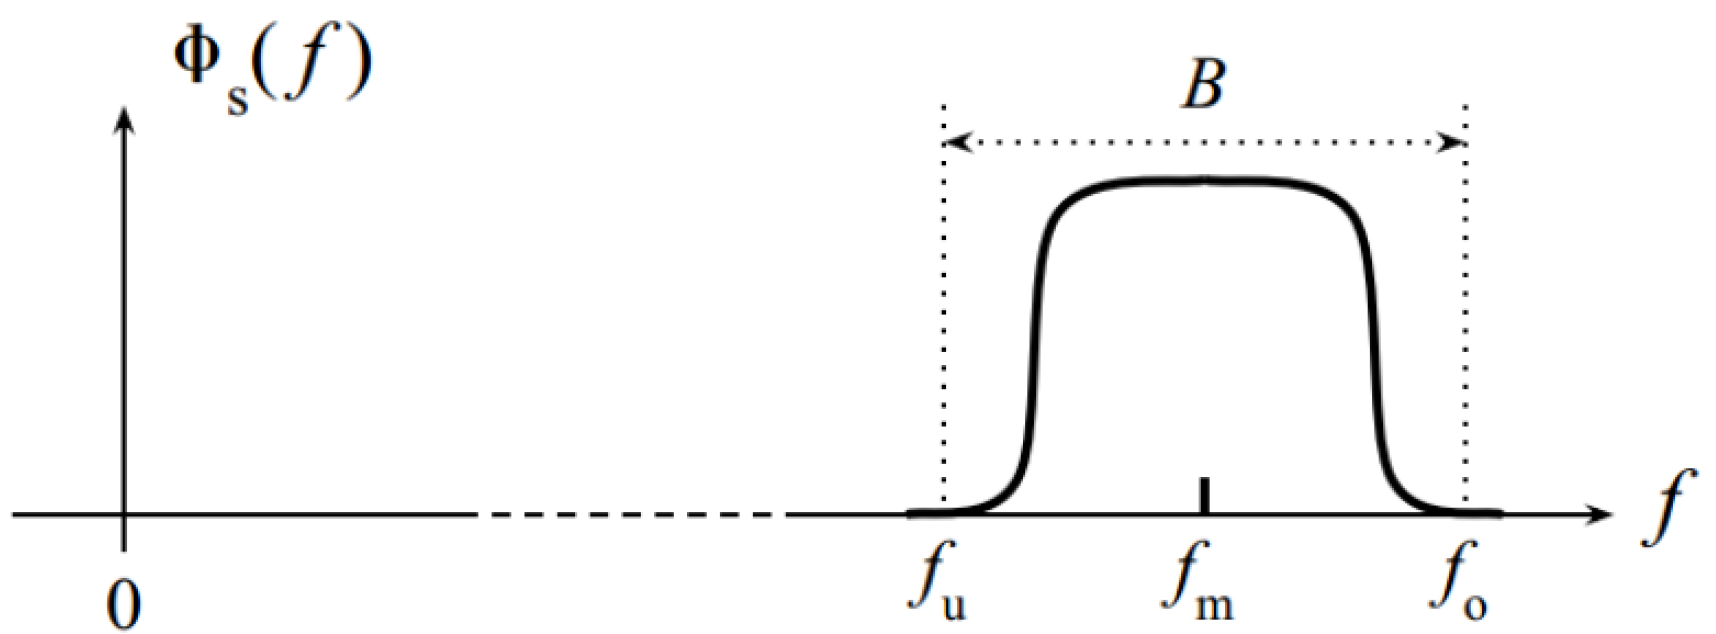
\includegraphics[width=0.8\textwidth]{./images/spek_bandp}
\end{center}

\section{Amplitudenmodulation}
Trägermodulation:
\[
	s_{RF}(t) = s(t) \cdot \cos(2\pi f_{RF} t)
\]
Träger:
\[
	\cos(2\pi f_{RF} t)	= \frac{\e^{\im 2 \pi f_{RF} t} + \e^{-\im 2 \pi f_{RF} t}}{2}
\]
Spektrum:
\begin{center}
	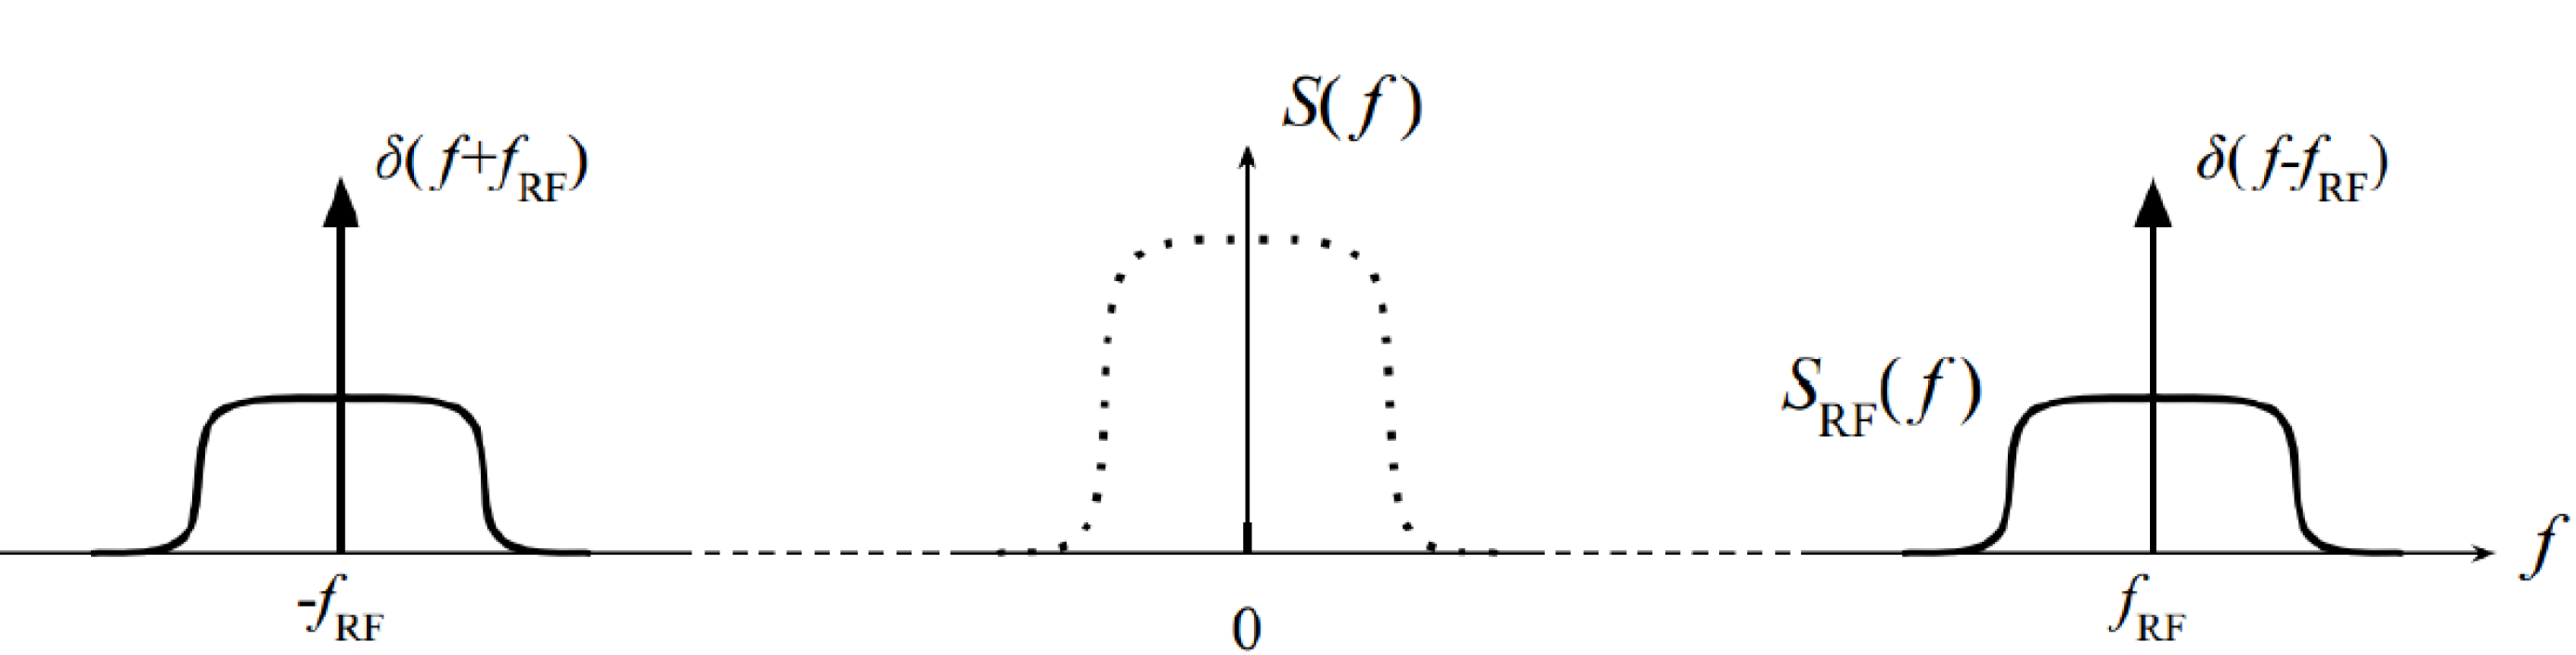
\includegraphics[width=.8\textwidth]{images/spek_band.png}
\end{center}

\section{Digitale Modulation}
mittlere Symbolenergie: $\varepsilon_s$ \\
mittlere Bitenergie: $ \varepsilon_B = \frac{\varepsilon_s}{\textrm{Anzahl Bit pro Symbol}} $ \\
minimale euklidische Distanz zwischen zwei Signalpunkten: $ d $
\section{Binäre Amplitudenumtastung (On-Off Keying)}
Basisband:
\[
	s(t) = \sum_{k} a_k \cdot p(t-kT_b) \qquad , a_k \in \lbrace 0,1 \rbrace
\]
~\\
Bandpasssignal:
\[
	s_{RF}(t) = s(t) \cos(2\pi f_{RF} t)
\]
~\\
Signalraum:\\
\begin{center}
\begin{tikzpicture}[scale=.9]
    \draw[->] (-1,0) -- (3,0);
    \draw[fill] (0,0) circle (2pt);
    \node[below] at (0,-.25) {0};
    \draw[fill] (2,0) circle (2pt);
    \node[below] at (2,-.25) {1};
    \node at (3.5,1) {$\varepsilon_s=0.5$};
\end{tikzpicture}
\end{center}

\section{Binäre Phasenumtastung (BPSK)}
Basisband:
\[
	s(t) = \sum_{k} a_k \cdot p(t-kT_b) \qquad , a_k \in \lbrace -1,1 \rbrace
\]
~\\
Bandpasssignal:
\[
	s_{RF}(t) = s(t) \cos(2\pi f_{RF} t)
\]
~\\
Signalraum:\\
\begin{center}
\begin{tikzpicture}[scale=.9]
    \draw[->] (-3,0) -- (3,0);
    \draw[-] (0,.1) -- (0,-.1);
    \draw[fill] (-2,0) circle (2pt);
    \node[below] at (-2,-.25) {-1};
    \draw[fill] (2,0) circle (2pt);
    \node[below] at (2,-.25) {1};
    \node at (3.5,1) {$\varepsilon_s=1$};
\end{tikzpicture}
\end{center}

\section{Amplitudenumtastung (PAM, AM, ASK)}
Basisband:
\[
	s(t) = \sum_{k} a_k \cdot p(t-kT_b) \qquad , a_k \in \lbrace -\frac{M-1}{2}, \ldots, \frac{M-1}{2} \rbrace
\]
~\\
Bandpasssignal:
\[
	s_{RF}(t) = s(t) \cos(2\pi f_{RF} t)
\]
~\\
Signalraum:\\
\begin{center}
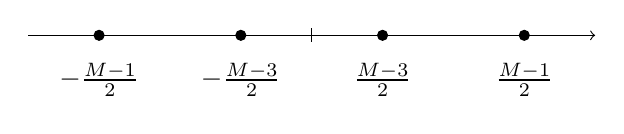
\begin{tikzpicture}[scale=.9]
    \draw[->] (-4,0) -- (4,0);
    \draw[-] (0,.1) -- (0,-.1);
    \draw[fill] (-3,0) circle (2pt);
	    \node[below] at (-3,-.25) {$-\frac{M-1}{2}$};
    \draw[fill] (-1,0) circle (2pt);
	    \node[below] at (-1,-.25) {$-\frac{M-3}{2}$};
	  \draw[fill] (1,0) circle (2pt);
	 	    \node[below] at (1,-.25) {$\frac{M-3}{2}$};
    \draw[fill] (3,0) circle (2pt);
	    \node[below] at (3,-.25) {$\frac{M-1}{2}$};
\end{tikzpicture}
\end{center}

\section{Phasenmodulation (PSK)}
Basisband:
\[
	s(t) = \sum_{k} a_k \cdot p(t-kT_b) 
	\qquad , a_k \in \left\lbrace \e^{\frac{\im 2 \pi 0}{M}}, \e^{\frac{\im 2 \pi 1}{M}}, \ldots,
	\e^{\frac{\im 2 \pi (M-1)}{M}} \right\rbrace
\]
~\\
Bandpasssignal:
\[
	s_{RF}(t) = \Re\lbrace s(t)\rbrace \cos(2\pi f_{RF} t)
		- \Im\lbrace s(t)\rbrace \sin(2\pi f_{RF} t)
\]
~\\
Signalraum:\\
\begin{center}
\begin{tikzpicture}[scale=.9]
   	\draw[->] (-1.5,0) -- (1.5,0) node[below] {\small$Re$};
   	\draw[->] (0,-1.5) -- (0,1.5) node[above right] {\small$Im$};
    \draw[dotted] (0,0) circle (1);	
    \draw[fill] (-1,0) circle (2pt);
    \draw[fill] (-.707,.707) circle (2pt);
    \draw[fill] (0,1) circle (2pt);
    \draw[fill] (.707,.707) circle (2pt);
    \draw[fill] (1,0) circle (2pt);
    \draw[fill] (.707,-.707) circle (2pt);
    \draw[fill] (0,-1) circle (2pt);
    \draw[fill] (-.707,-.707) circle (2pt);
    \node at (2,2) {$\varepsilon_s = 1$};
\end{tikzpicture}
\end{center}

\section{Minimum Shift Keying}
Basisband:
\[\begin{aligned}
	\phi_s(t) = \pi h \left(\sum_{n=-\infty}^{k-1} a_n + a_k \frac{t-kT_s}{T_s} \right)
		\textrm{ mit }
		k=\left\lfloor\frac{t}{T_s}\right\rfloor,\\
		a_k \in \left\lbrace \pm 1, \pm 3,\ldots, \pm (M-1) \right\rbrace
\end{aligned}\]
~\\
Bandpasssignal:
\[
	s_{RF}(t) = \Re\lbrace s(t)\rbrace \cos(2\pi f_{RF} t)
		- \Im\lbrace s(t)\rbrace \sin(2\pi f_{RF} t)
\]

\section{Quadraturamplitudenmodulation (QAM)}
Basisband:
\[
	s(t) = \sum_{k} a_k \cdot p(t-kT_s)
\]
~\\
Bandpasssignal:
\[
	s_{RF}(t) = \Re\lbrace s(t)\rbrace \cos(2\pi f_{RF} t)
		- \Im\lbrace s(t)\rbrace \sin(2\pi f_{RF} t)
\]
~\\
Modulator/Demoudlation:
\begin{center}
	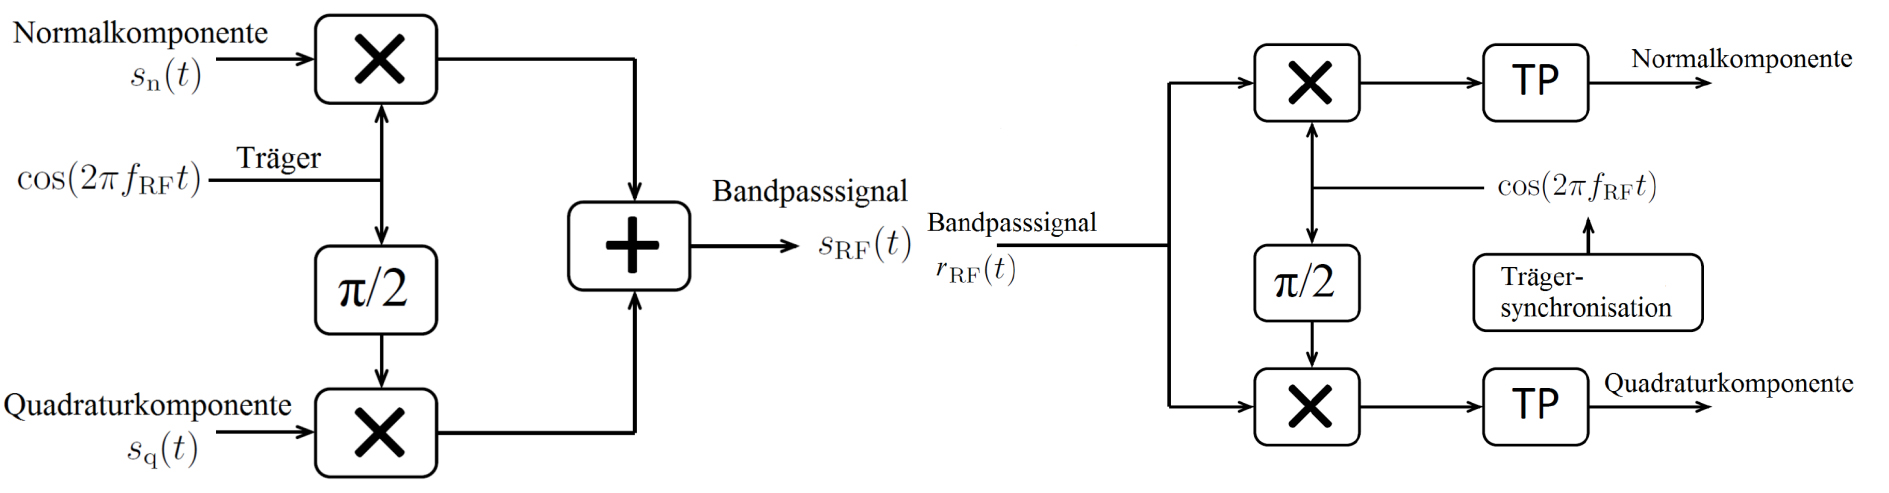
\includegraphics[width=.9\textwidth]{images/qam_modde.jpg}
\end{center}
~\\Bsp: 16-QAM:\\
\begin{center}
\begin{tikzpicture}[scale=.5]
   	\draw[->] (-4,0) -- (4,0) node[below] {\small$I$};
   	\draw[->] (0,-4) -- (0,4) node[above right] {\small$Q$};
    \draw[dotted] (-4,2) -- (4,2);	
    \draw[dotted] (-4,-2) -- (4,-2);    
    \draw[dotted] (-2,-4) -- (-2,4);	
    \draw[dotted] (2,-4) -- (2,4);	
    
    \draw[fill] (-3,3) circle (2pt);
    \draw[fill] (-1,3) circle (2pt);
    \draw[fill] (1,3) circle (2pt);
    \draw[fill] (3,3) circle (2pt);
    
    \draw[fill] (-3,1) circle (2pt);
    \draw[fill] (-1,1) circle (2pt);
    \draw[fill] (1,1) circle (2pt);
    \draw[fill] (3,1) circle (2pt);
    
    \draw[fill] (-3,-1) circle (2pt);
    \draw[fill] (-1,-1) circle (2pt);
    \draw[fill] (1,-1) circle (2pt);
    \draw[fill] (3,-1) circle (2pt);
        
    \draw[fill] (-3,-3) circle (2pt);
    \draw[fill] (-1,-3) circle (2pt);
    \draw[fill] (1,-3) circle (2pt);
    \draw[fill] (3,-3) circle (2pt);
\end{tikzpicture}
\end{center}

\begin{center}
	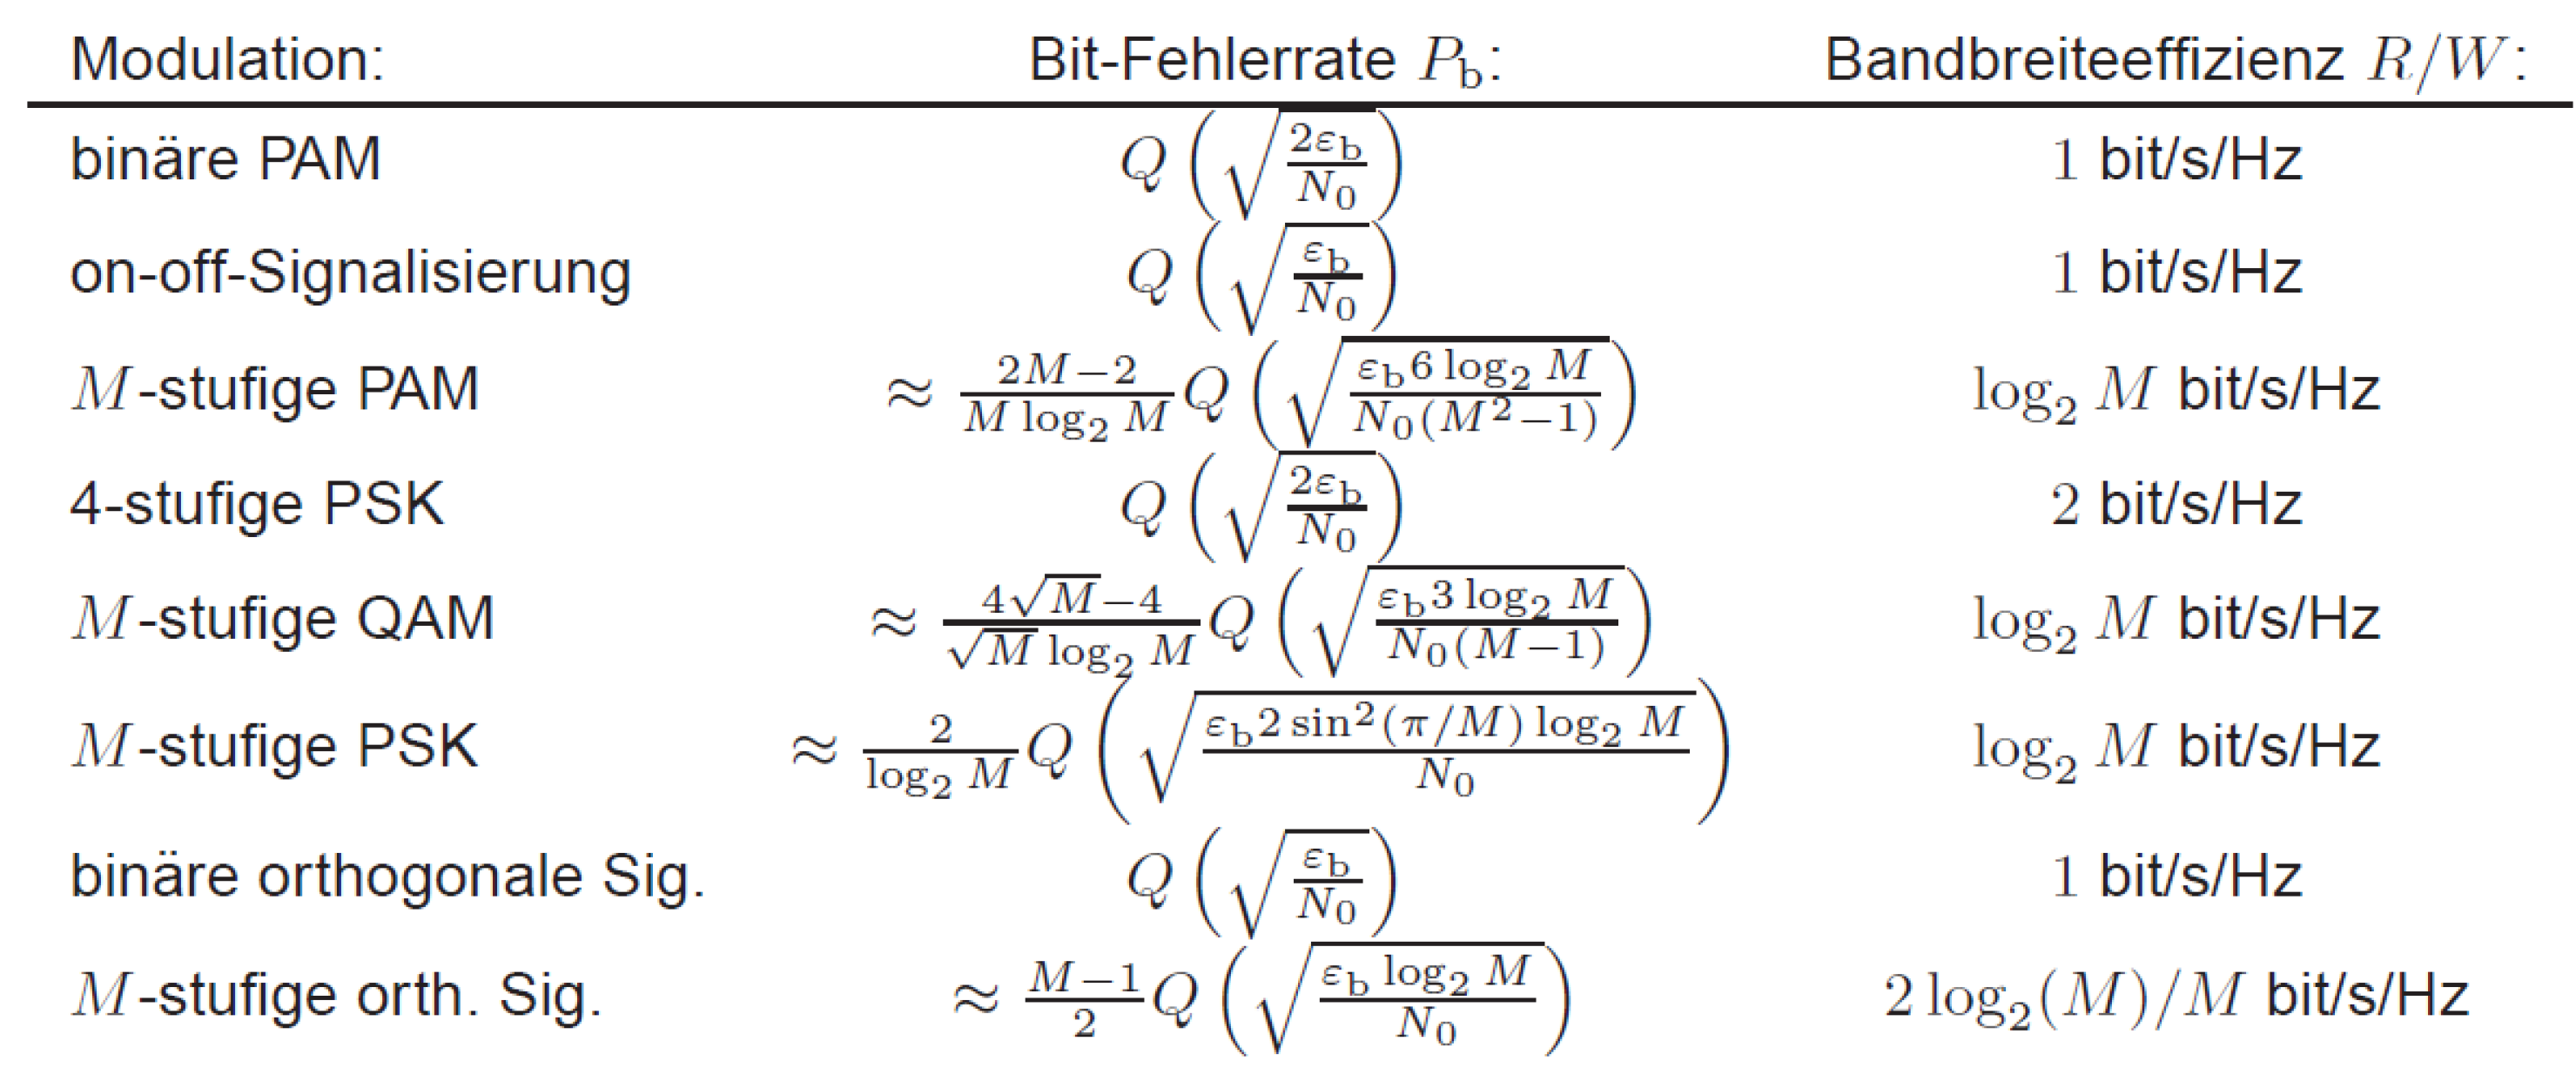
\includegraphics[width=.9\textwidth]{./images/fehler.png}
\end{center}
\chapter{Übertragung}
Bandbreite des Sendesignals:
\[ B \approx \frac{1}{T_S} \]

\begin{center}
	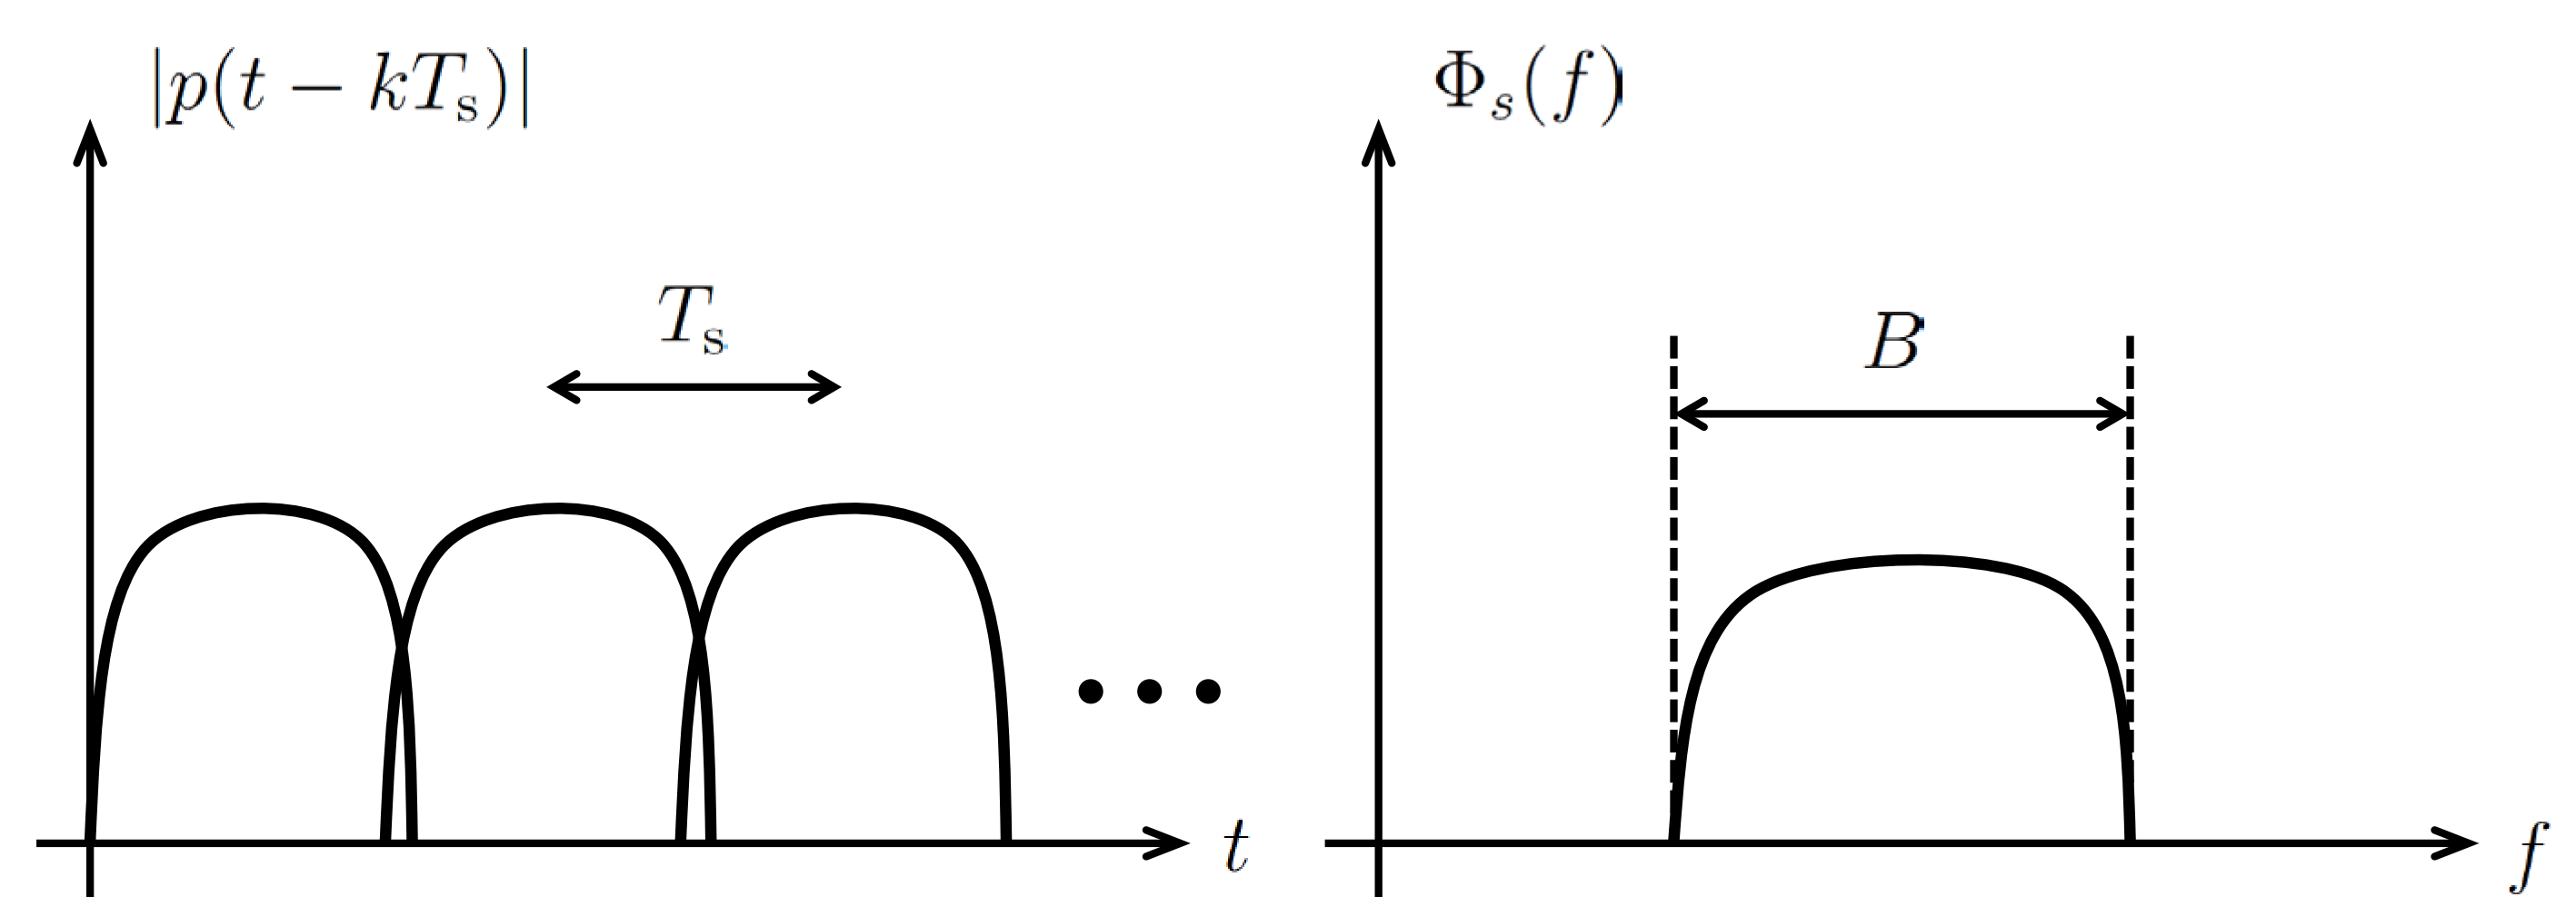
\includegraphics[width=.9\textwidth]{../fig/eintrager.png}
\end{center}

\section{Mehrweg-Ausbreitung}
Kohärenzbandbreite des Kanals:
\[ B_c \approx \frac{1}{\tau_m} \]

\begin{center}
	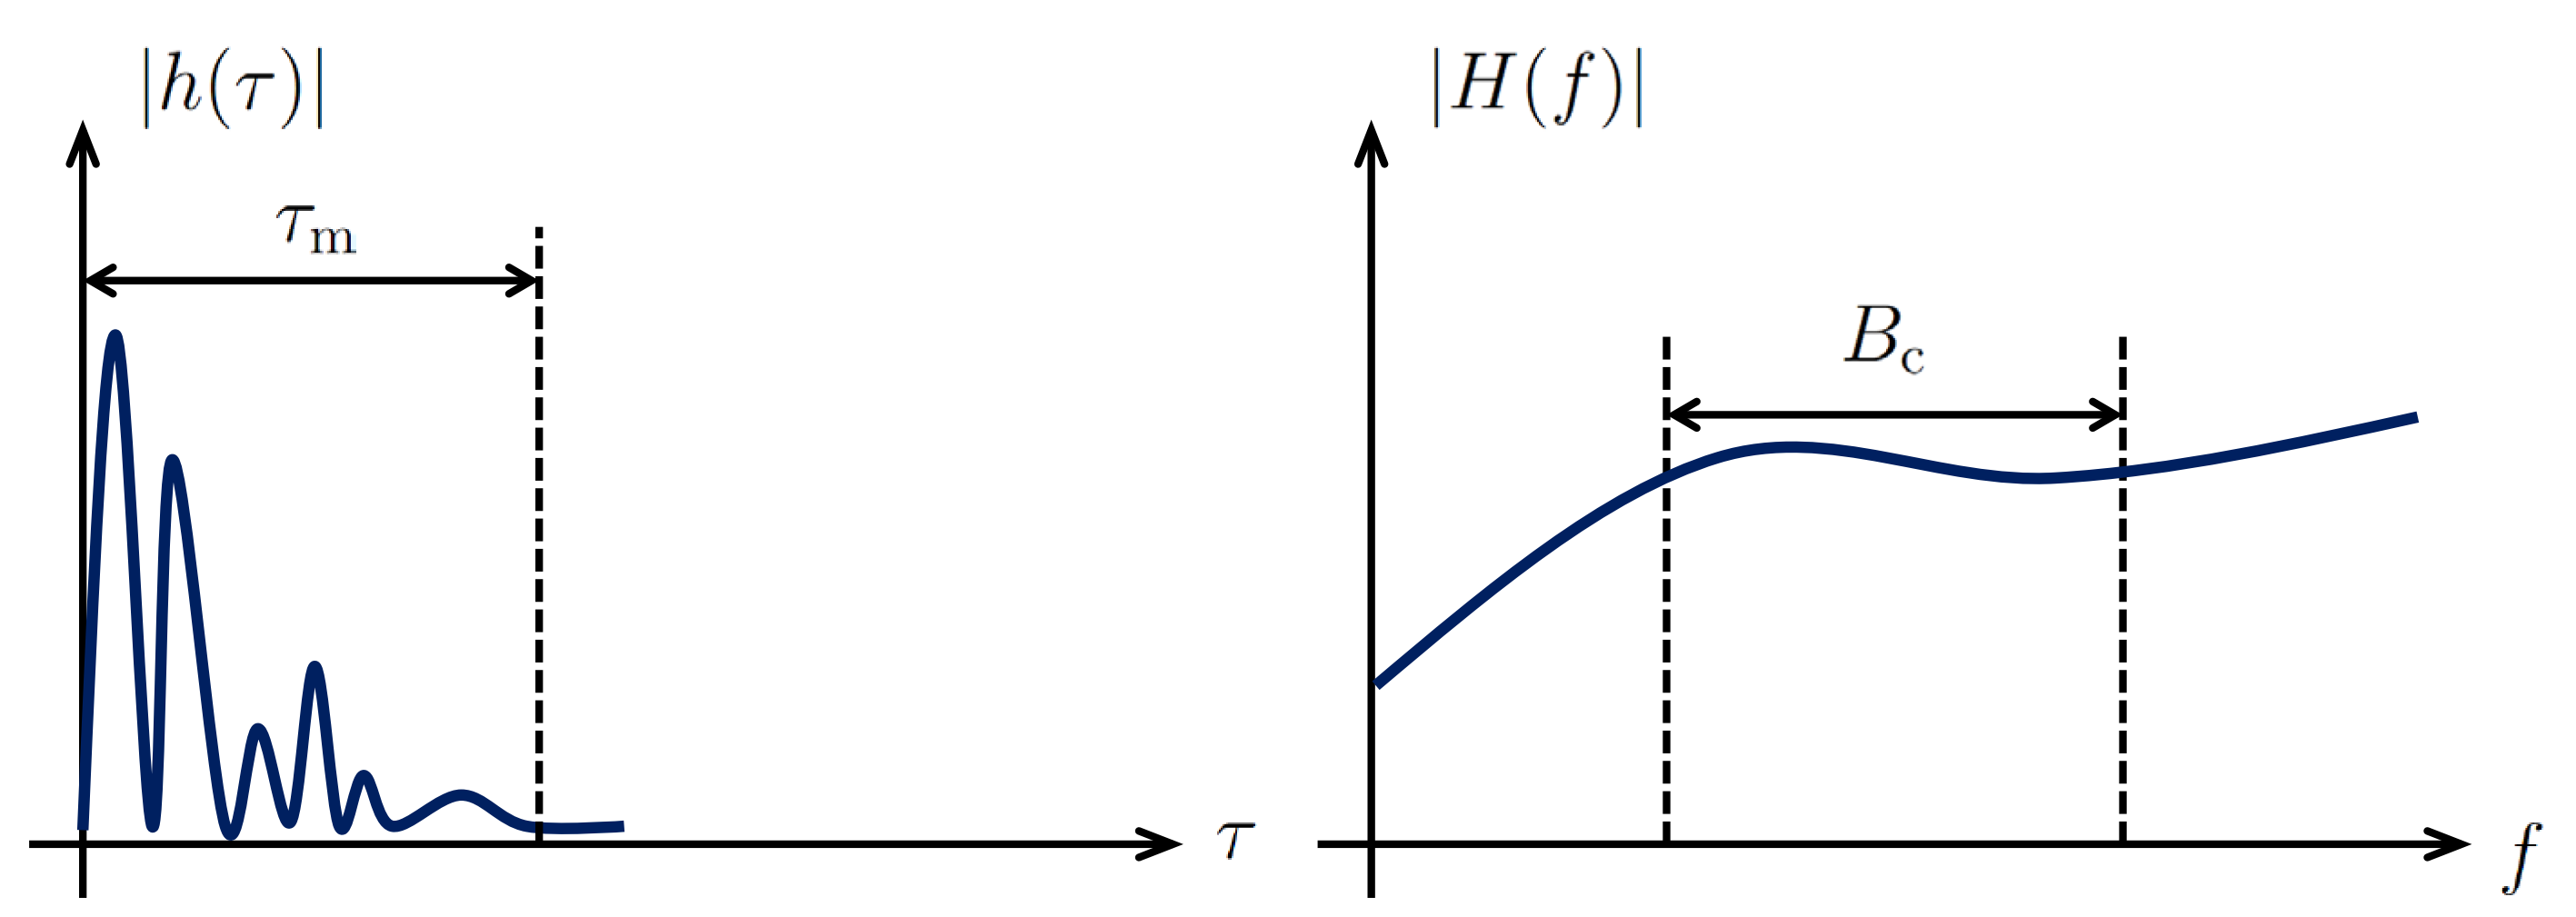
\includegraphics[width=.9\textwidth]{../fig/mehrweg.png}
\end{center}

\section{Verzerrung}
Impuls am Empfänger:
\[ q(t) = (p * h)(t) \]
~\\
Leistungsdichtespektrum des Empfangssignals:
\[ \Phi_r(f) = \Phi_s(f) \cdot |H(f)|^2 \]

\section{Schmalband vs. Breitband}
Symboldauer: $T_s$\\
Bandbreite: $B \approx \frac{1}{T_S}$\\
Multipath Spread: $\tau_m$\\
Kohärenzbandbreite: $B_c \approx \frac{1}{\tau_m}$\\
schmalbandige Übertragung: $\tau_m < T_s$\\
breitbandige Übertragung: $\tau_m > T_s$

\subsection{Schmalbandige Übertragung}
Impuls am Empfänger:
\[ q(t) \approx \alpha \cdot p(t) \]
~\\
Leistungsdichtespektrum des Empfangssignals:
\[ \Phi_r(f) \approx |\alpha|^2 \cdot \Phi_s(f) \]
~\\
\[ \tau_m < T_s \qquad B < B_c \]
\begin{center}
	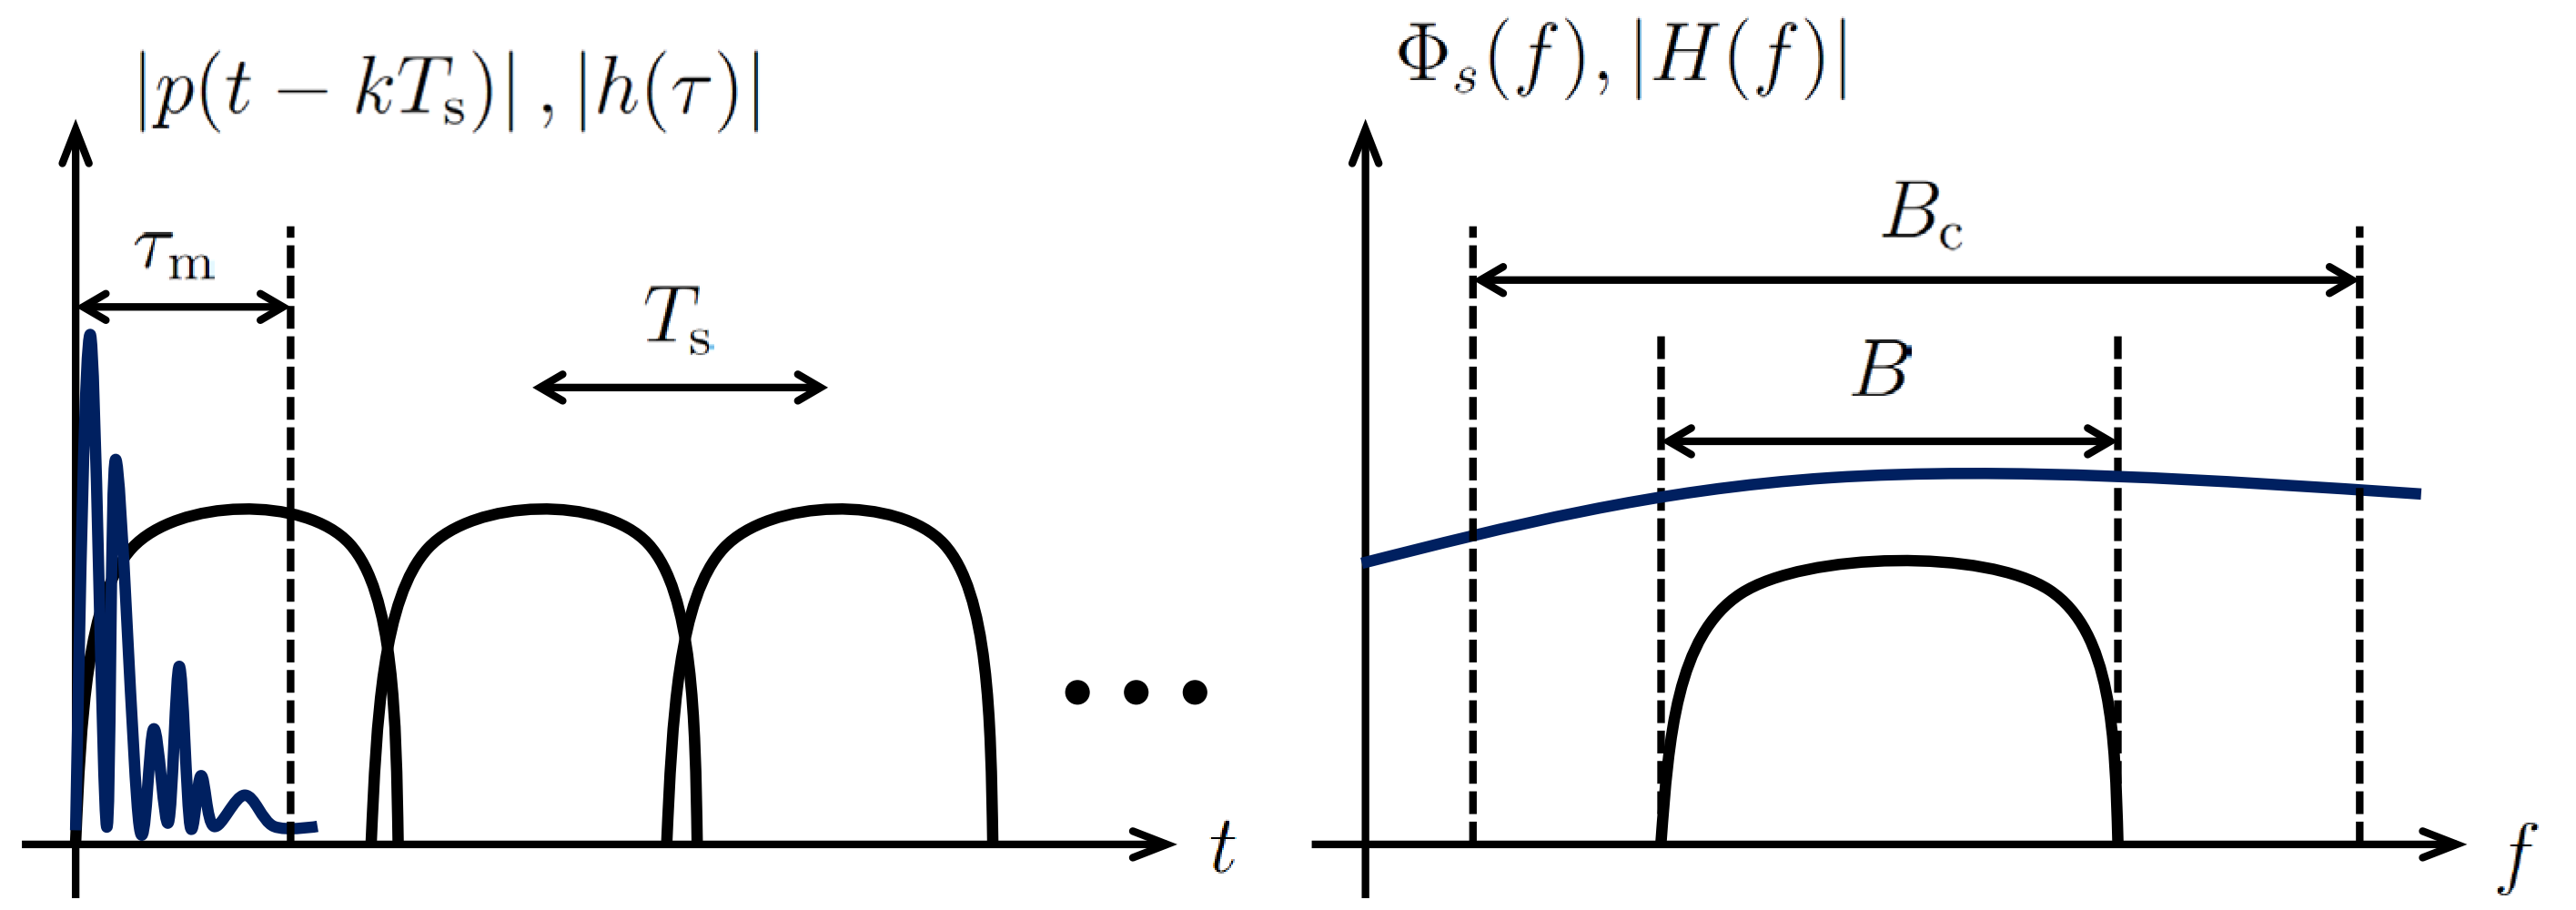
\includegraphics[width=.9\textwidth]{../fig/schmalband.png}
\end{center}
\begin{center}
	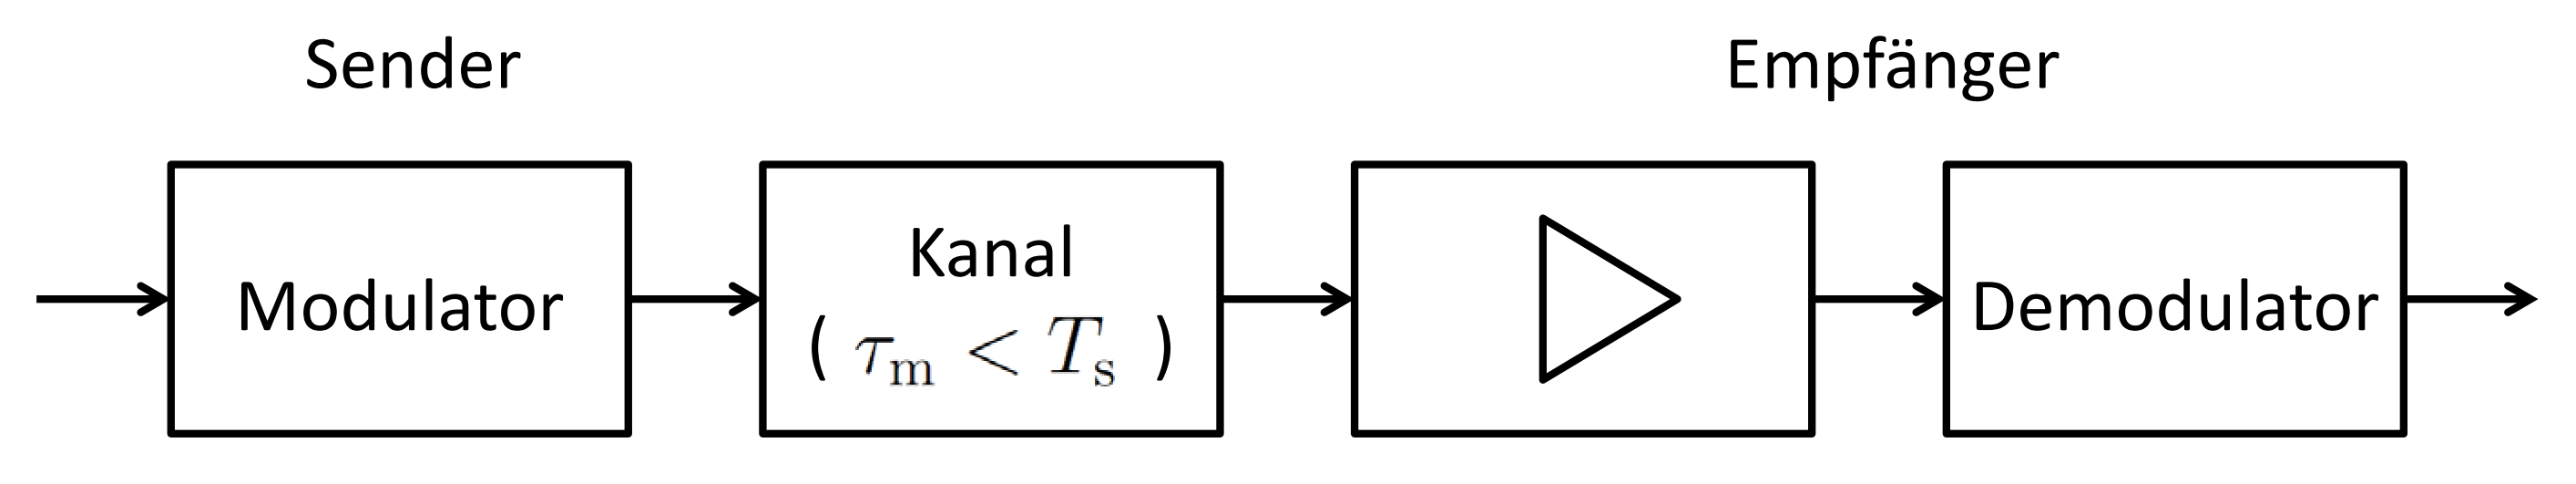
\includegraphics[width=.9\textwidth]{../fig/mod_schmalband.png}
\end{center}

\subsection{Breitbandige Übertragung}
Impuls am Empfänger:
\[ q(t) = (p*h)(t) \]
~\\
Leistungsdichtespektrum des Empfangssignals:
\[ \Phi_r(f) = \Phi_s(f) \cdot |H(f)|^2 \]
~\\
\[ \tau_m > T_s \qquad B > B_c \]
\begin{center}
	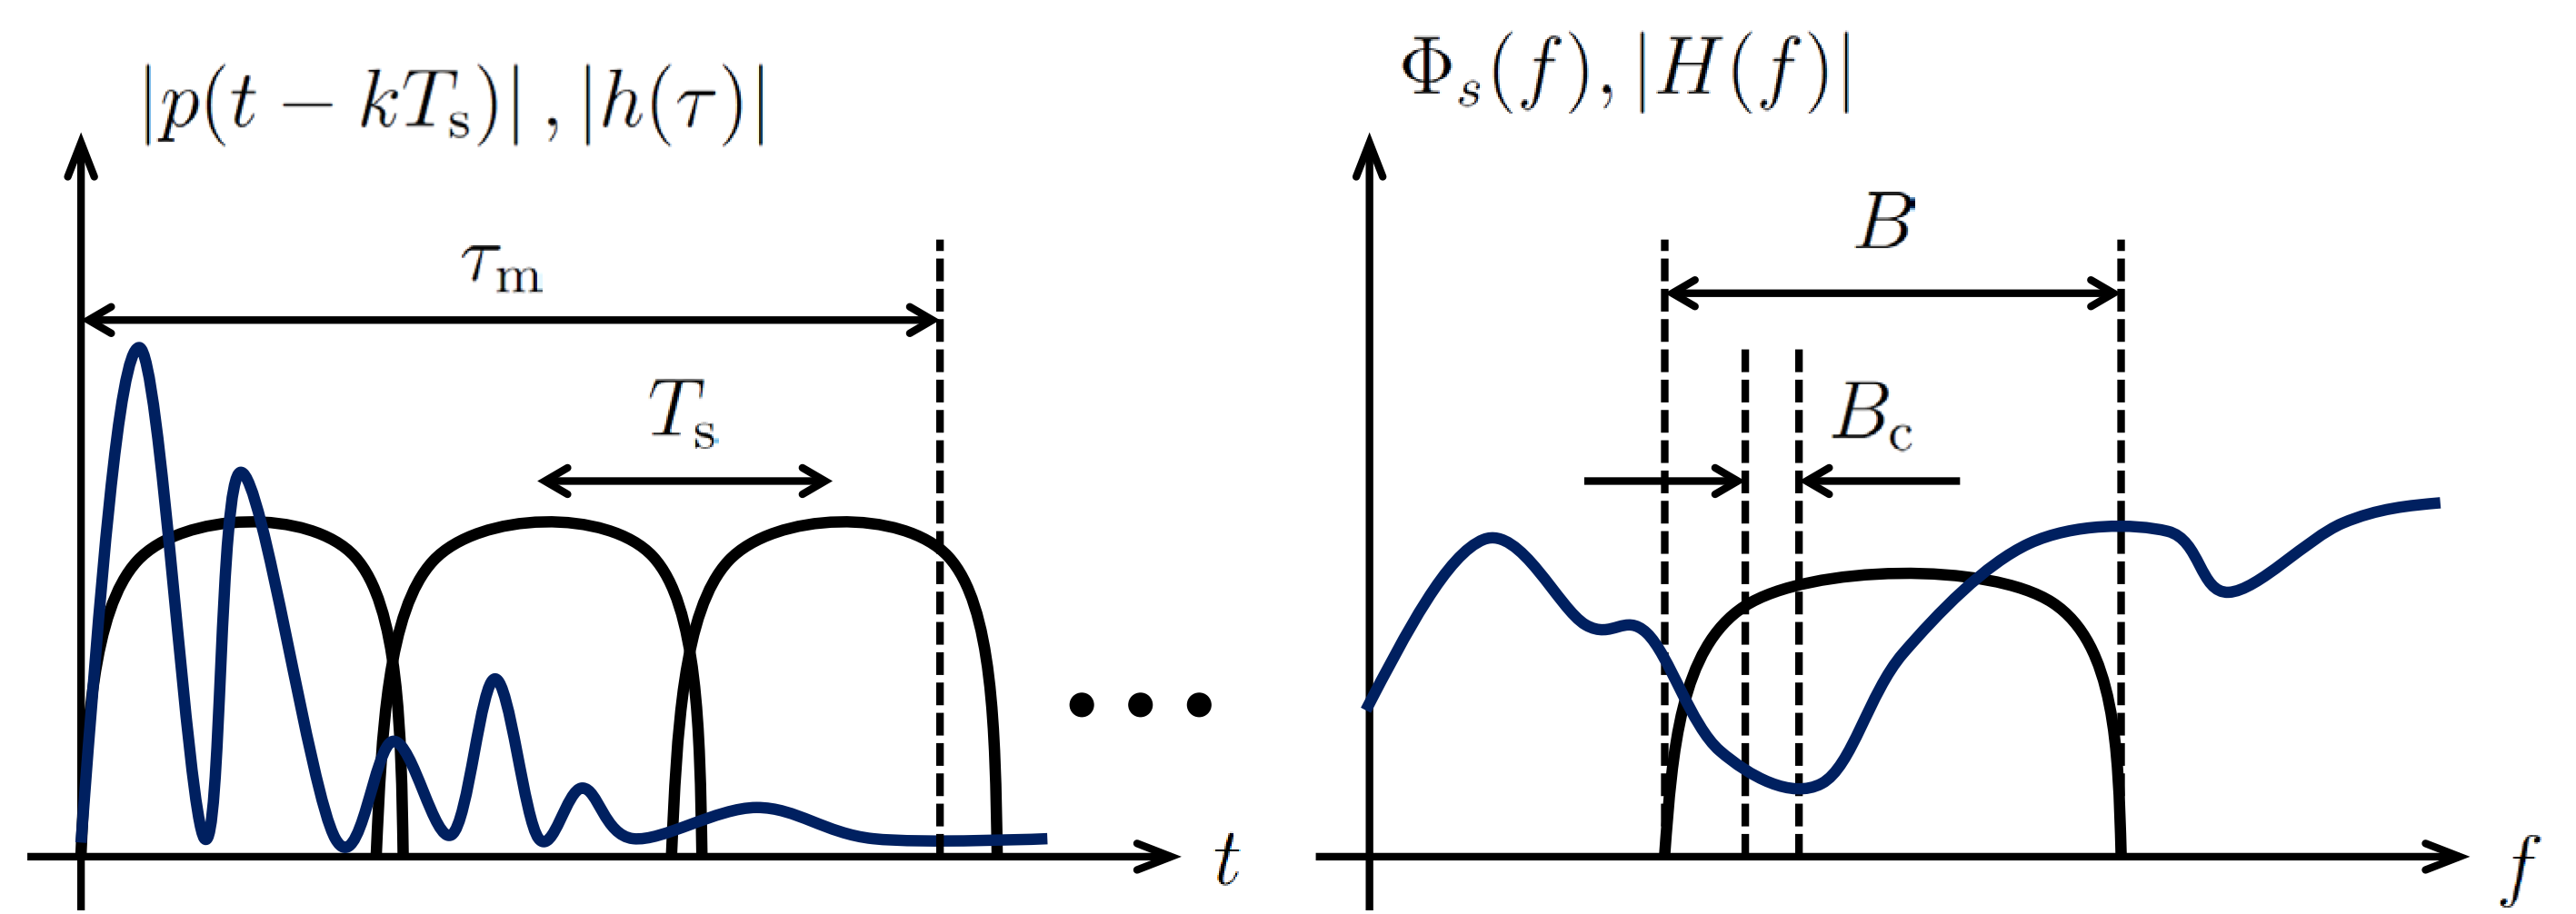
\includegraphics[width=.9\textwidth]{../fig/breitband.png}
\end{center}
\begin{center}
	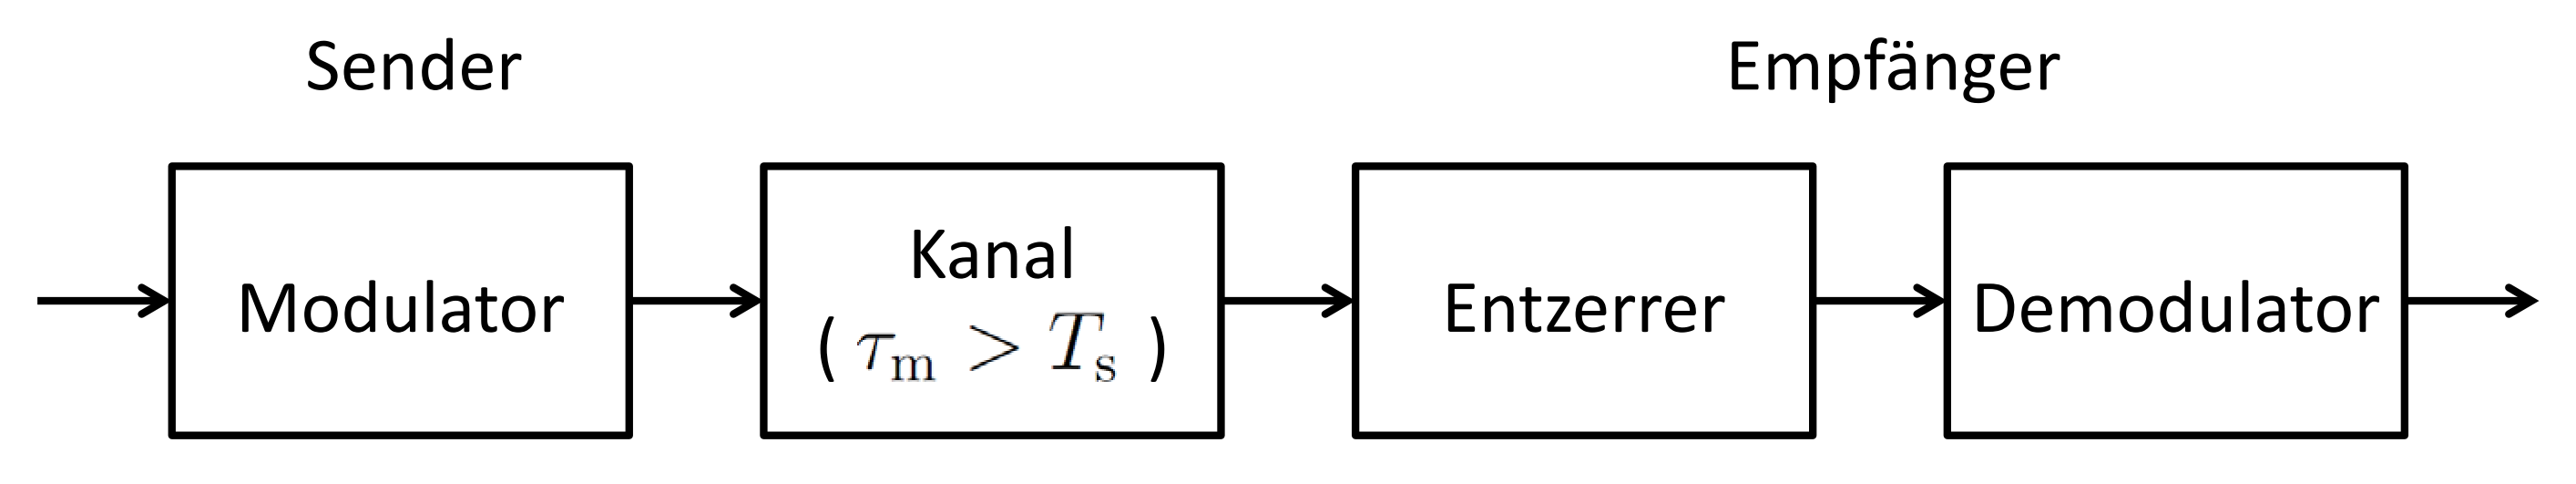
\includegraphics[width=.9\textwidth]{../fig/mod_breitband.png}
\end{center}

\section{Mehrträgerübertragung}
Bandbreite des Sendesignals: $B$\\
Bandbreite eines Unterträgers: $B_{sc}$

\begin{center}
	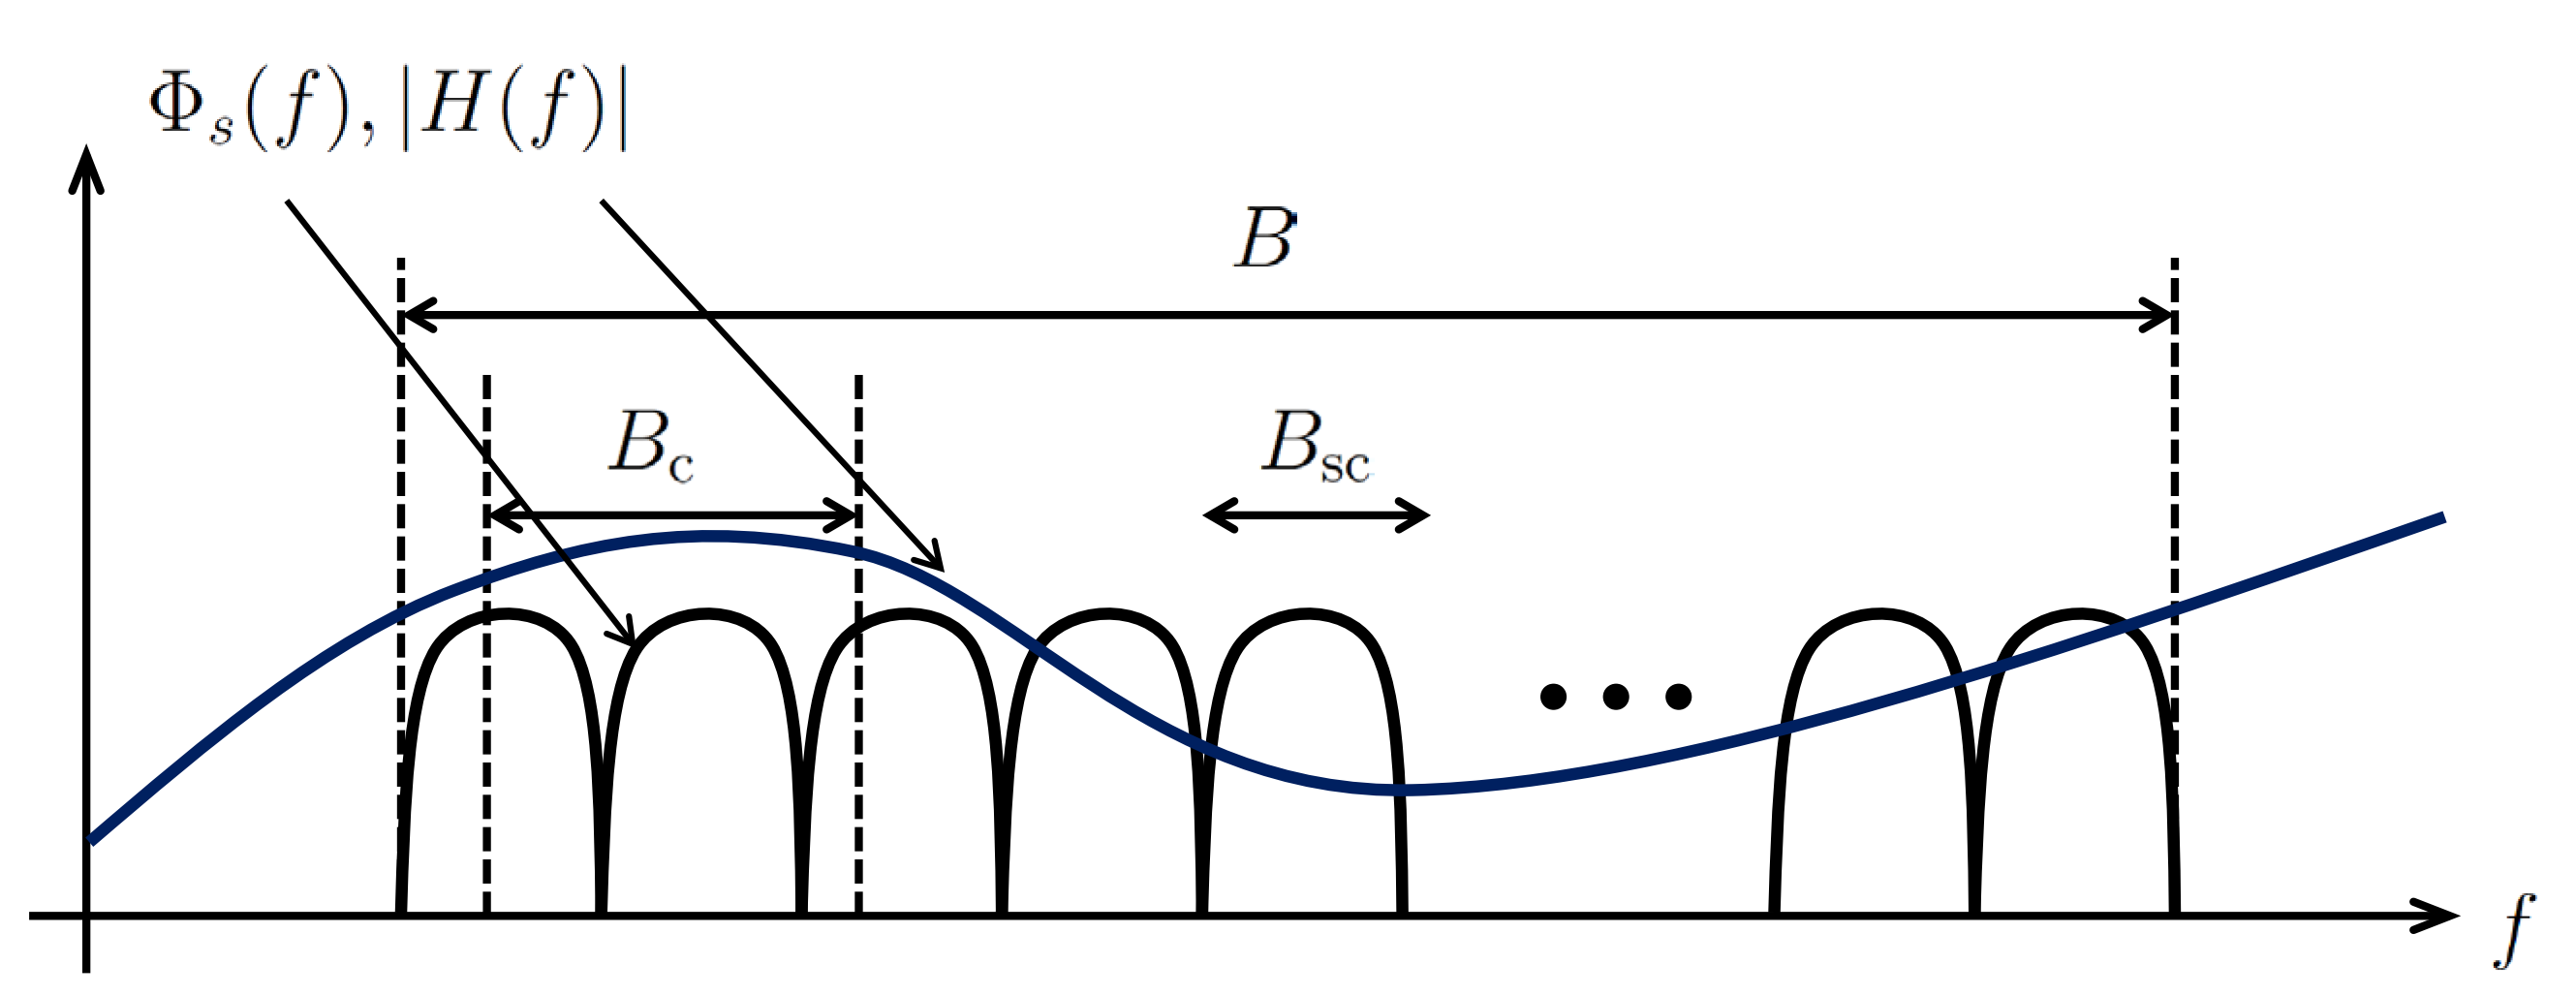
\includegraphics[width=.9\textwidth]{../fig/mehrtrager.png}
\end{center}

\section{OFDM}
Dauer des Kernsymbols: $T_{FFT}$ \\
Dauer des Schutzintervalls: $T_{cp}$ \\
Bedingung für interferenzfreien Empfang: $T_{cp} \geq \tau_m$
\begin{center}
	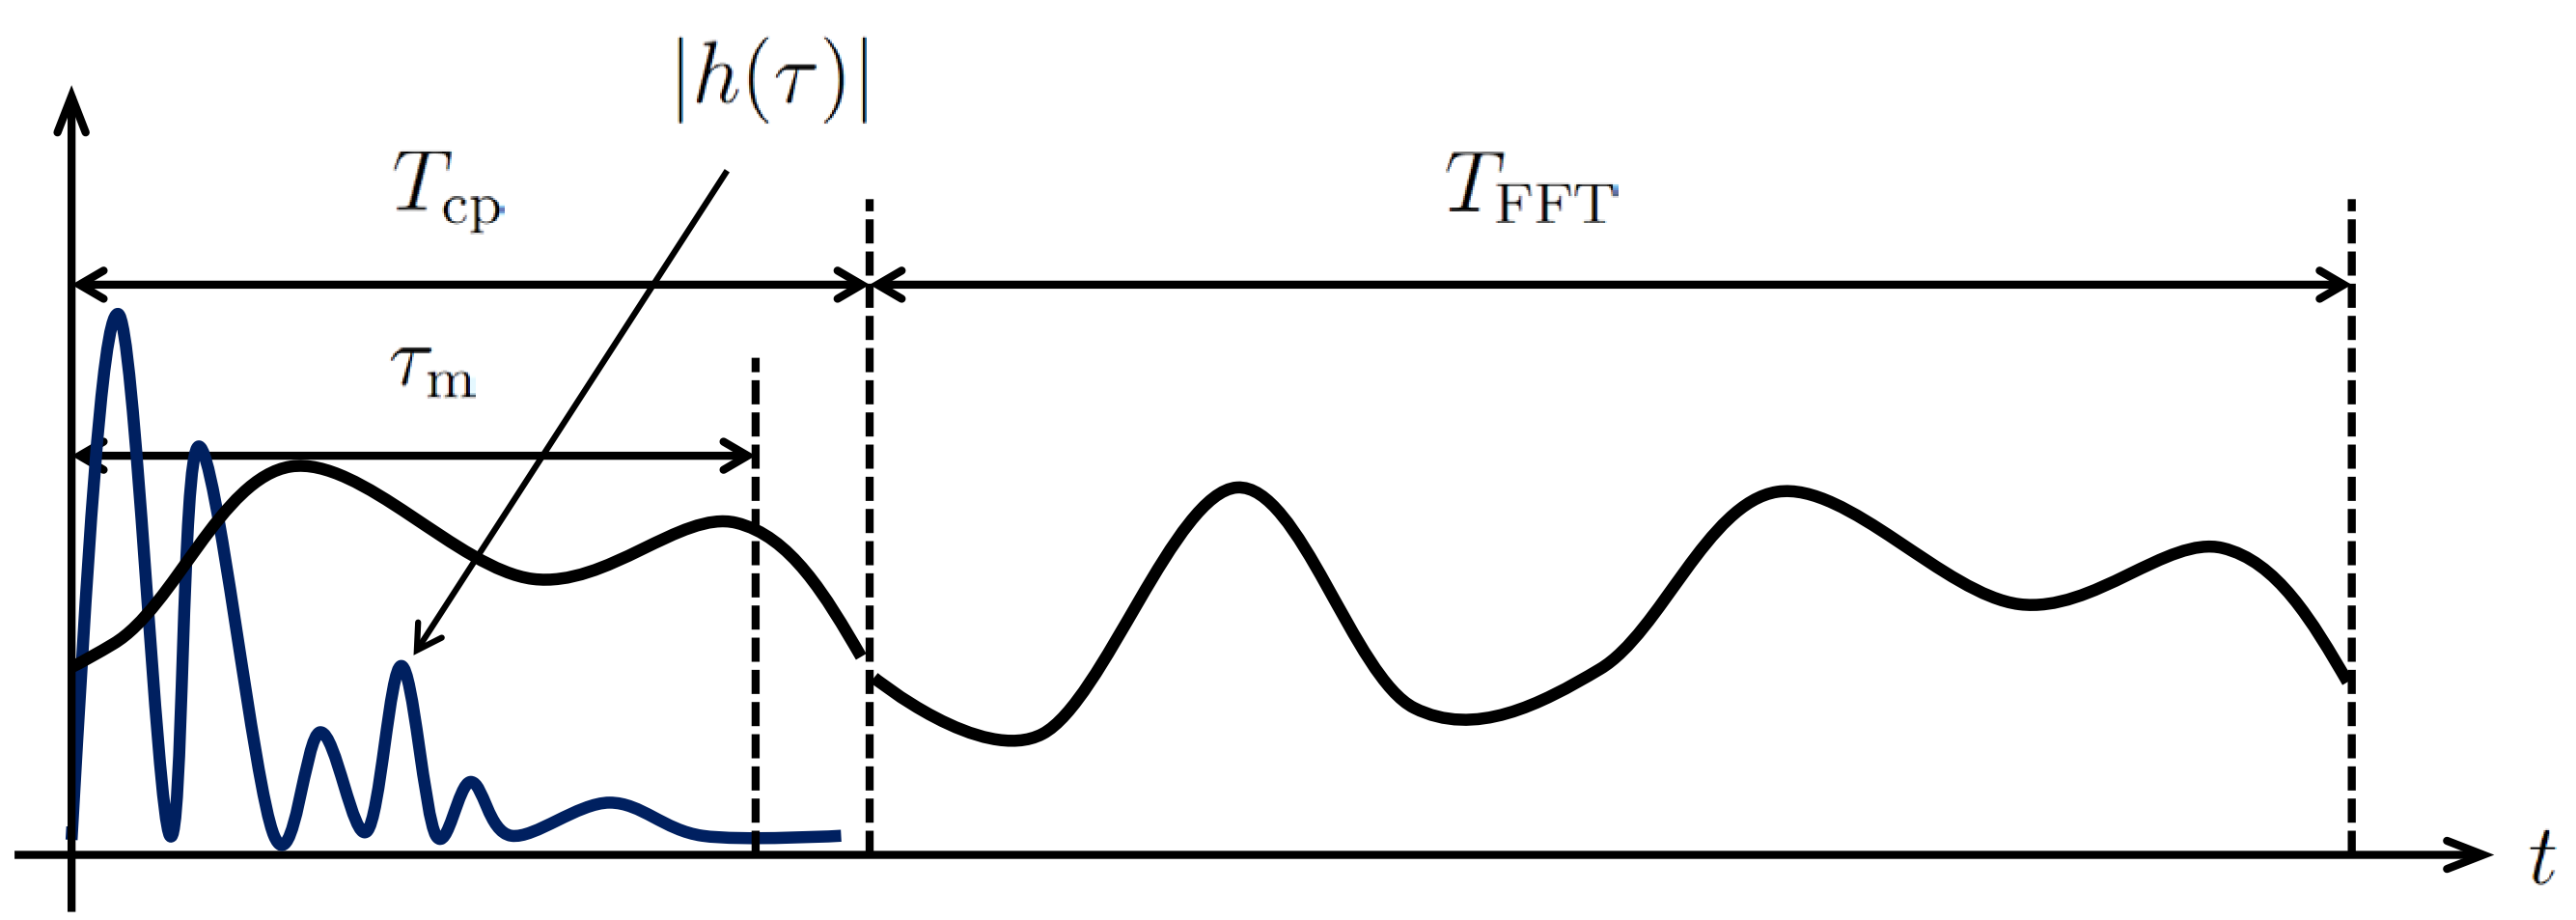
\includegraphics[width=.9\textwidth]{../fig/ofdm.png}
\end{center}
~\\
Bandbreite: $B$ \\
Unterträger: $K$ \\
Bandbreite Unterträger:
\[
	F = \frac{B}{K}
\]
~\\
Dauer des Kernsymbols:
\[
	T_{FFT} = \frac{1}{F}
\]
~\\
Dauer des Schutzintervalls:
\[
	T_{cp} \geq \frac{\textrm{längster Pfad [m]}}{3\cdot 10^8 \frac{m}{s}}
\]
~\\
Gesamtdauer:
\[
	T_{OFDM} = T_{cp} + T_{FFT}
\]
~\\
Bitrate:
\[ 
	R_b = \frac{K \cdot \textrm{Bit pro Symbol}}{T_{OFDM}}
\]
Spektrale Effizienz:
\[
	R/W = \frac{R_b}{B}
\]

\chapter{Matched Filter}
\begin{center}
	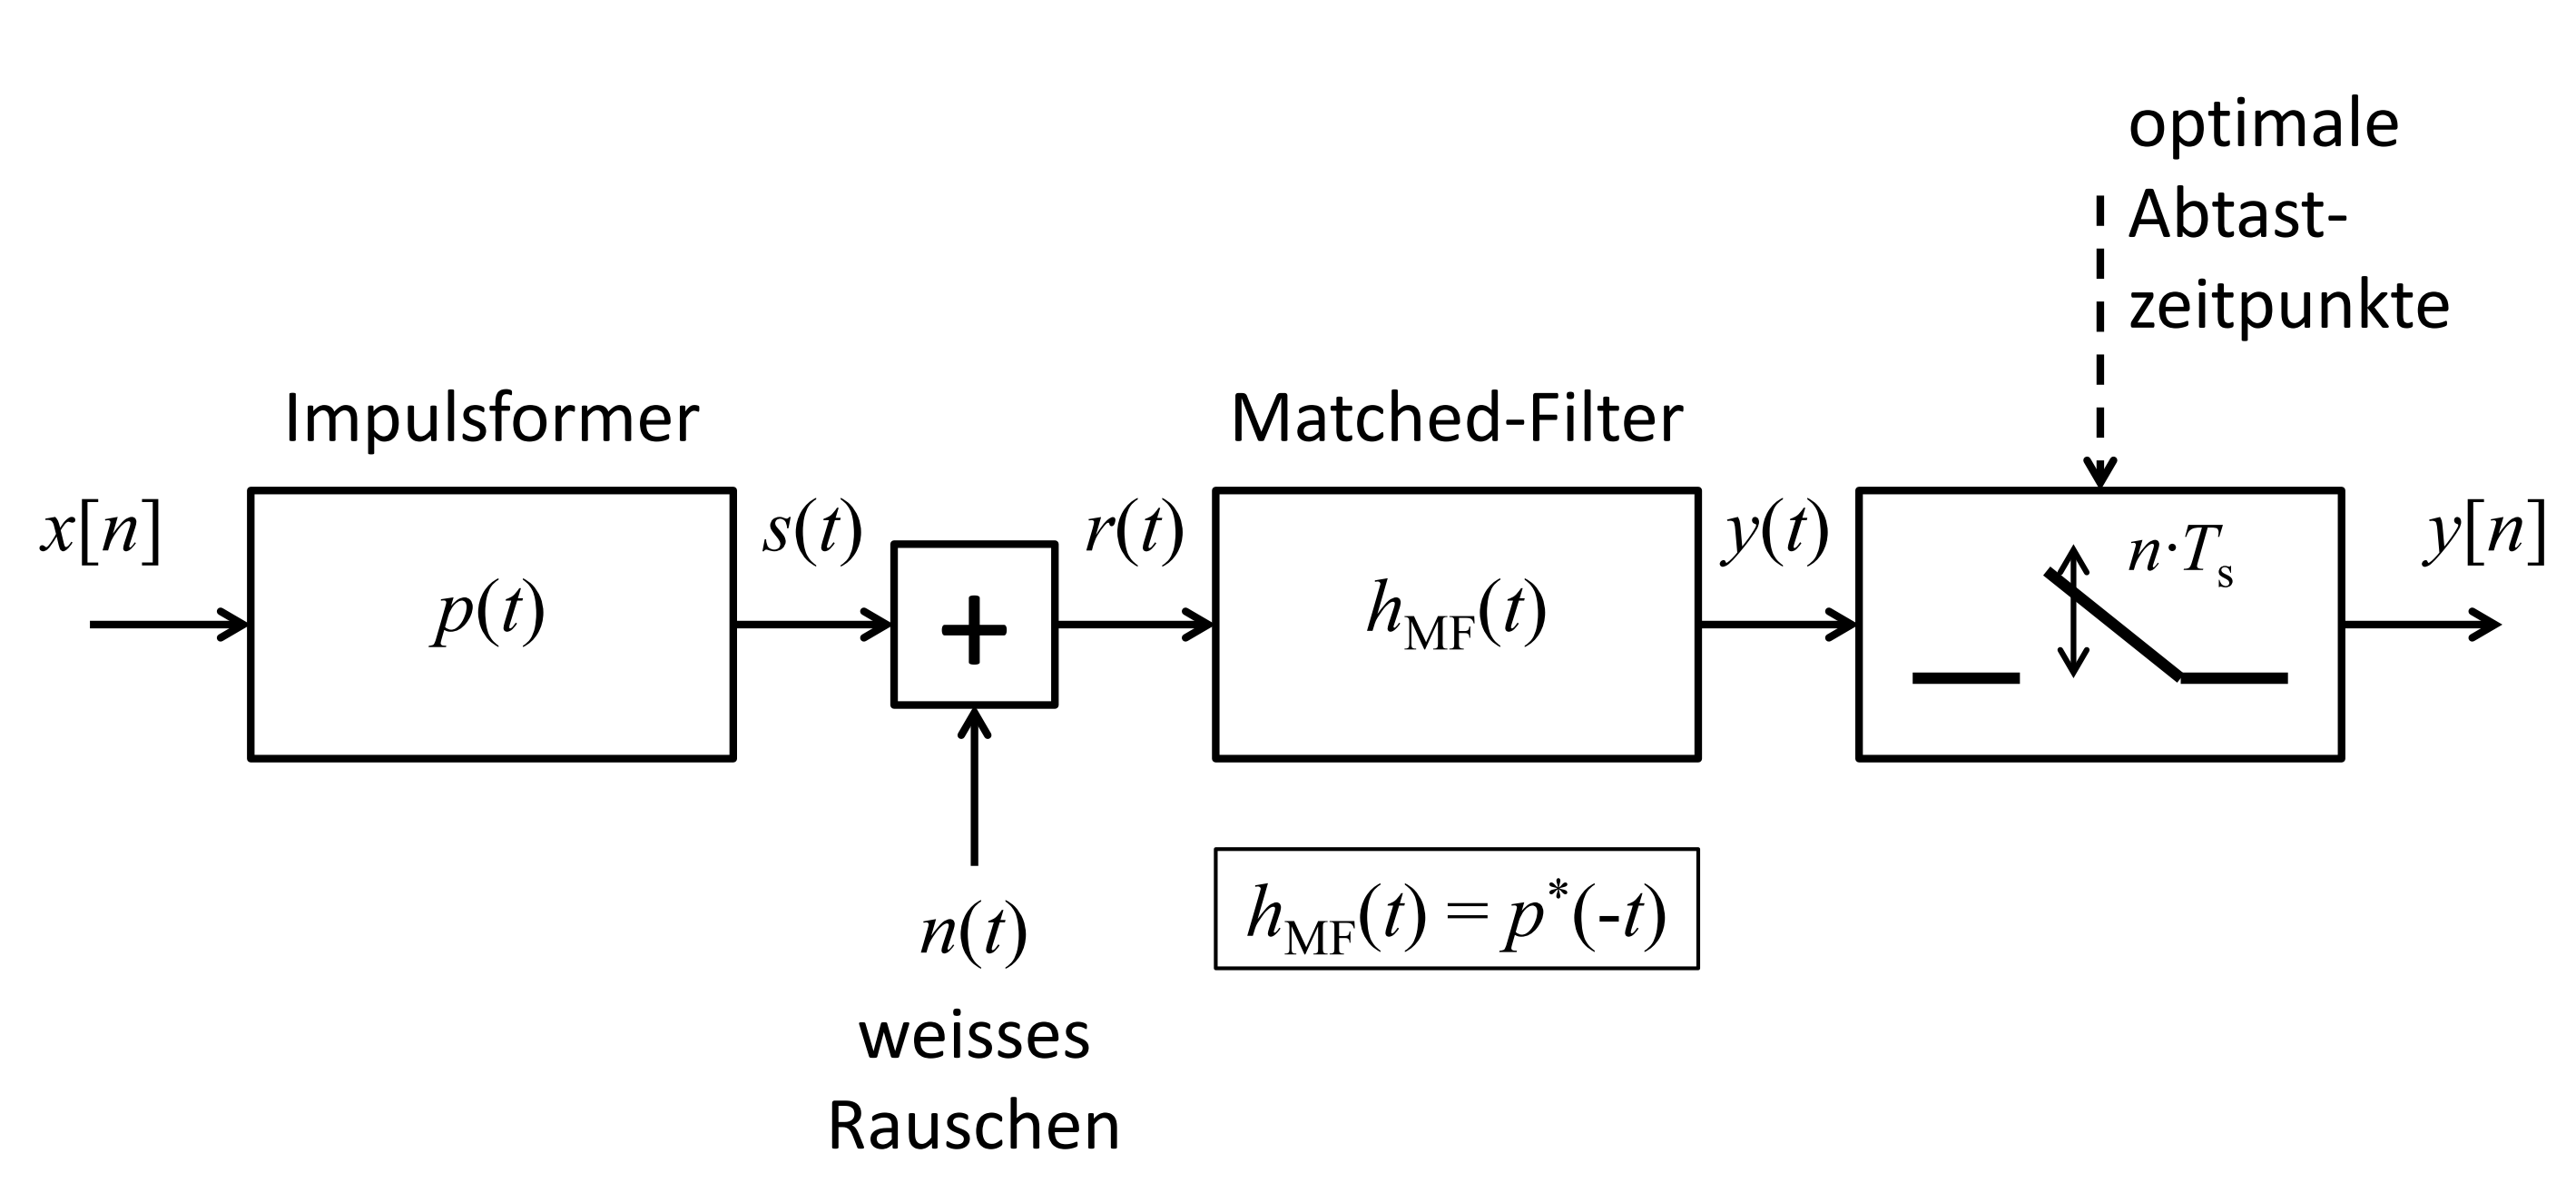
\includegraphics[width=.9\textwidth]{./images/matched}
\end{center}
~\\
Wahrscheinlichkeitsdichte mit Gauss:
\[
	f_X(x) = \frac{1}{\sqrt{2\pi\sigma^2}}\cdot\e^{-\frac{(x-m)^2}{2\sigma^2}}
\]
~\\
Q-Funktion:
\[
	Q(z) = \int_{z}^{\infty} \frac{1}{\sqrt{2\pi}}\e^{-\frac{x^2}{2}}\di x =
		\frac{1}{2}\textrm{erfc} \left( \frac{z}{\sqrt{2}} \right)
\]
~\\
Error-Funktion:
\[
	\textrm{erfc}(z) = \frac{2}{\sqrt{\pi}} \int_{z}^{\infty}\e^{-x^2}\di x = 2Q(\sqrt{2}z)
\]
~\\
$Y$ ist Gauss-Verteilt mit Mittelwert $m$ und Varianz $\sigma^2$:
\[
	P(Y\geq z) = Q\left(\frac{z-m}{\sigma}\right)
		= \frac{1}{2}\textrm{erfc}\left(\frac{z-m}{\sqrt{2}\sigma}\right)
\]

\section{Weisses gausssches Rauschen am Empfängerfilter}
\begin{center}
	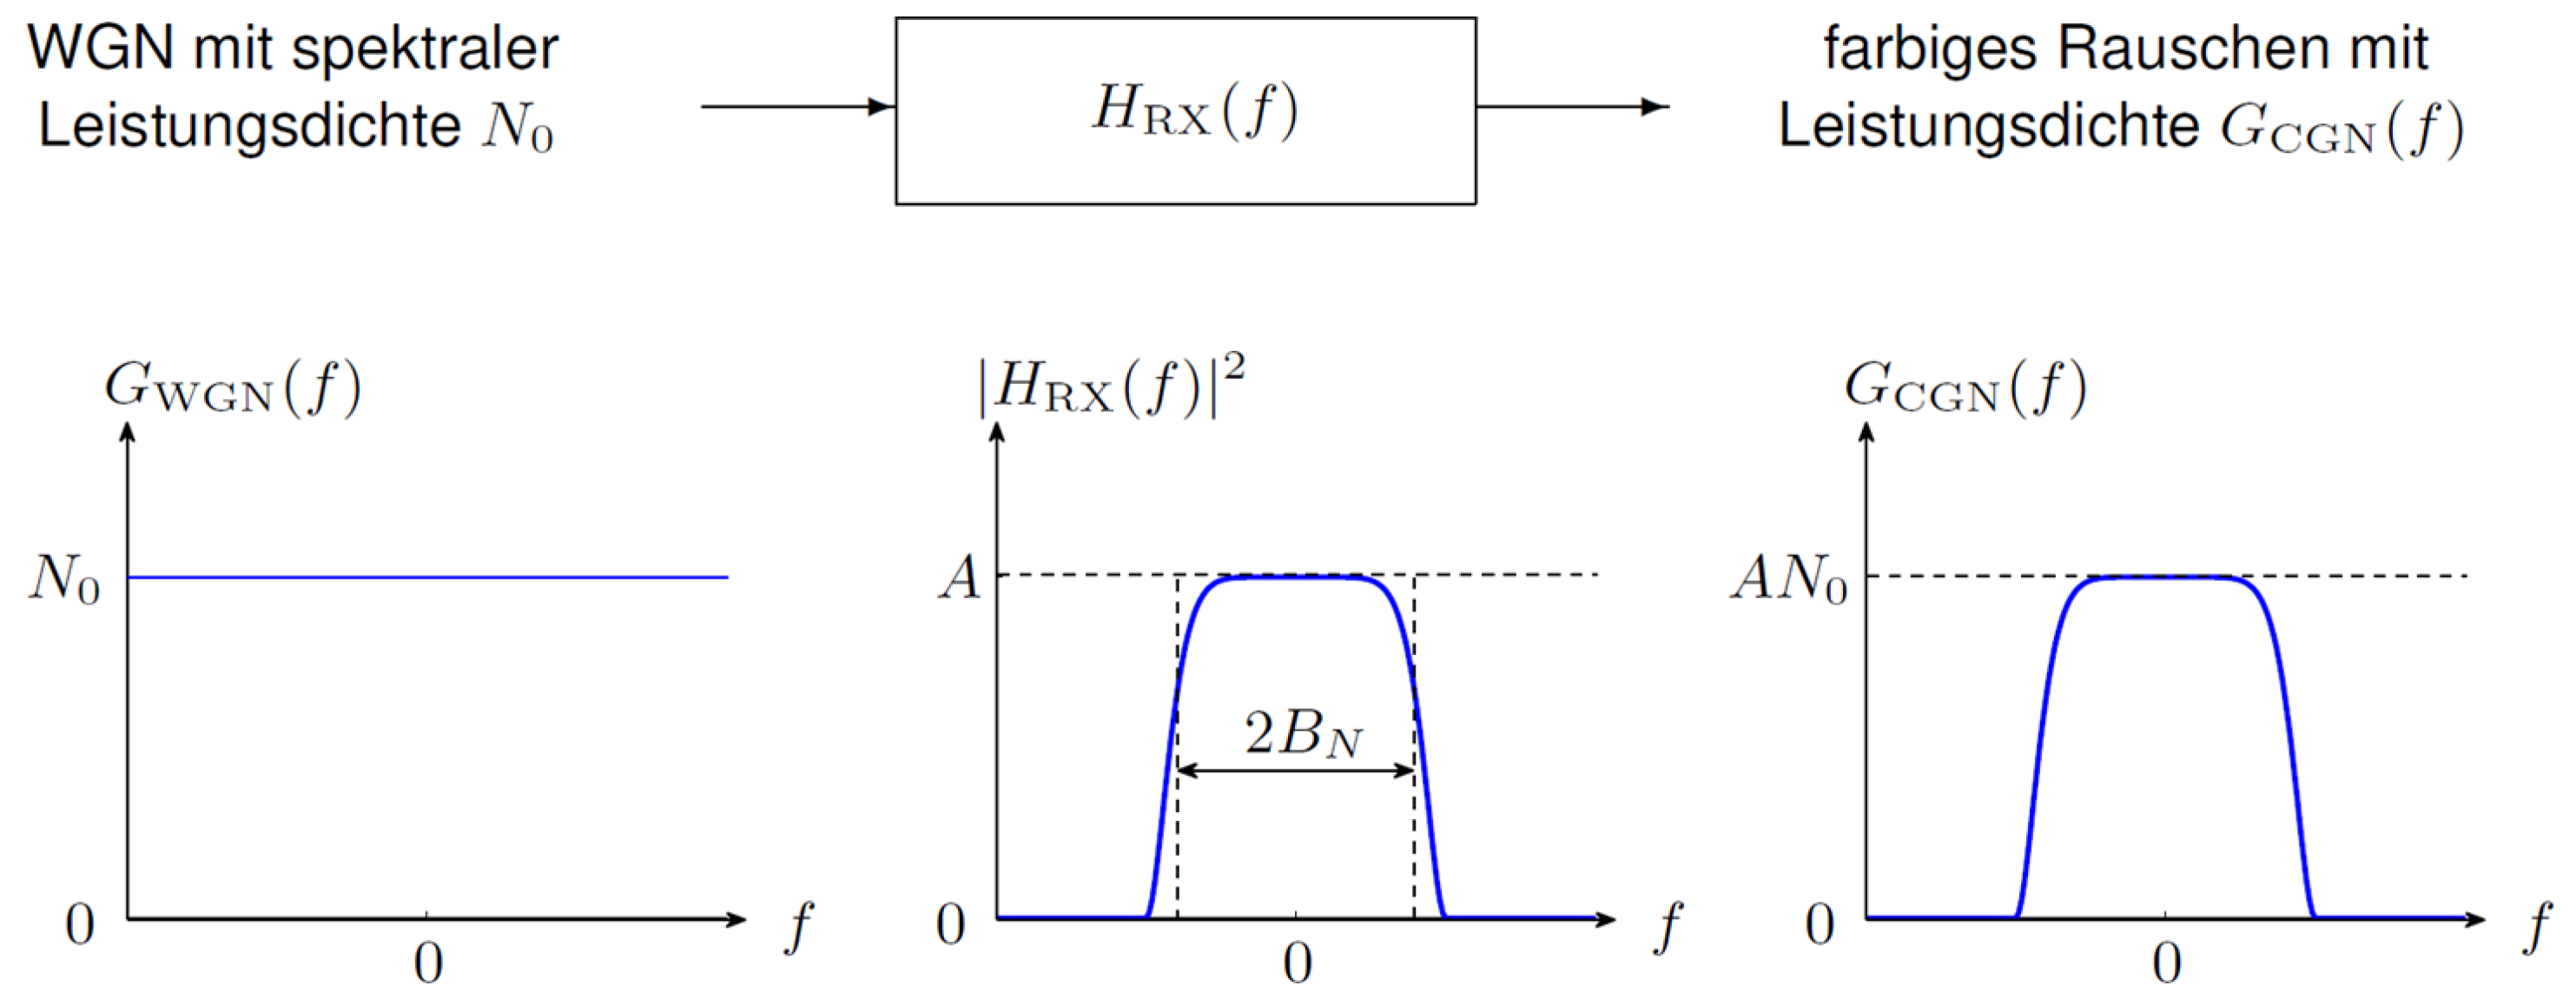
\includegraphics[width=.9\textwidth]{./images/wgn.png}
\end{center}
Äquivalente Rauschbandbreite des TP:
\[
	B_N = A^{-1} \int_{0}^{\infty}|H_{RX}(f)|^2 \di f
\]
~\\
Leistung des reellen Rauschsignals am Filterausgang:
\[
	\frac{N}{2} = N_0 \int_{0}^{\infty}|H_{RX}(f)|^2 \di f = N_0AB_N
\]

\begin{center}
	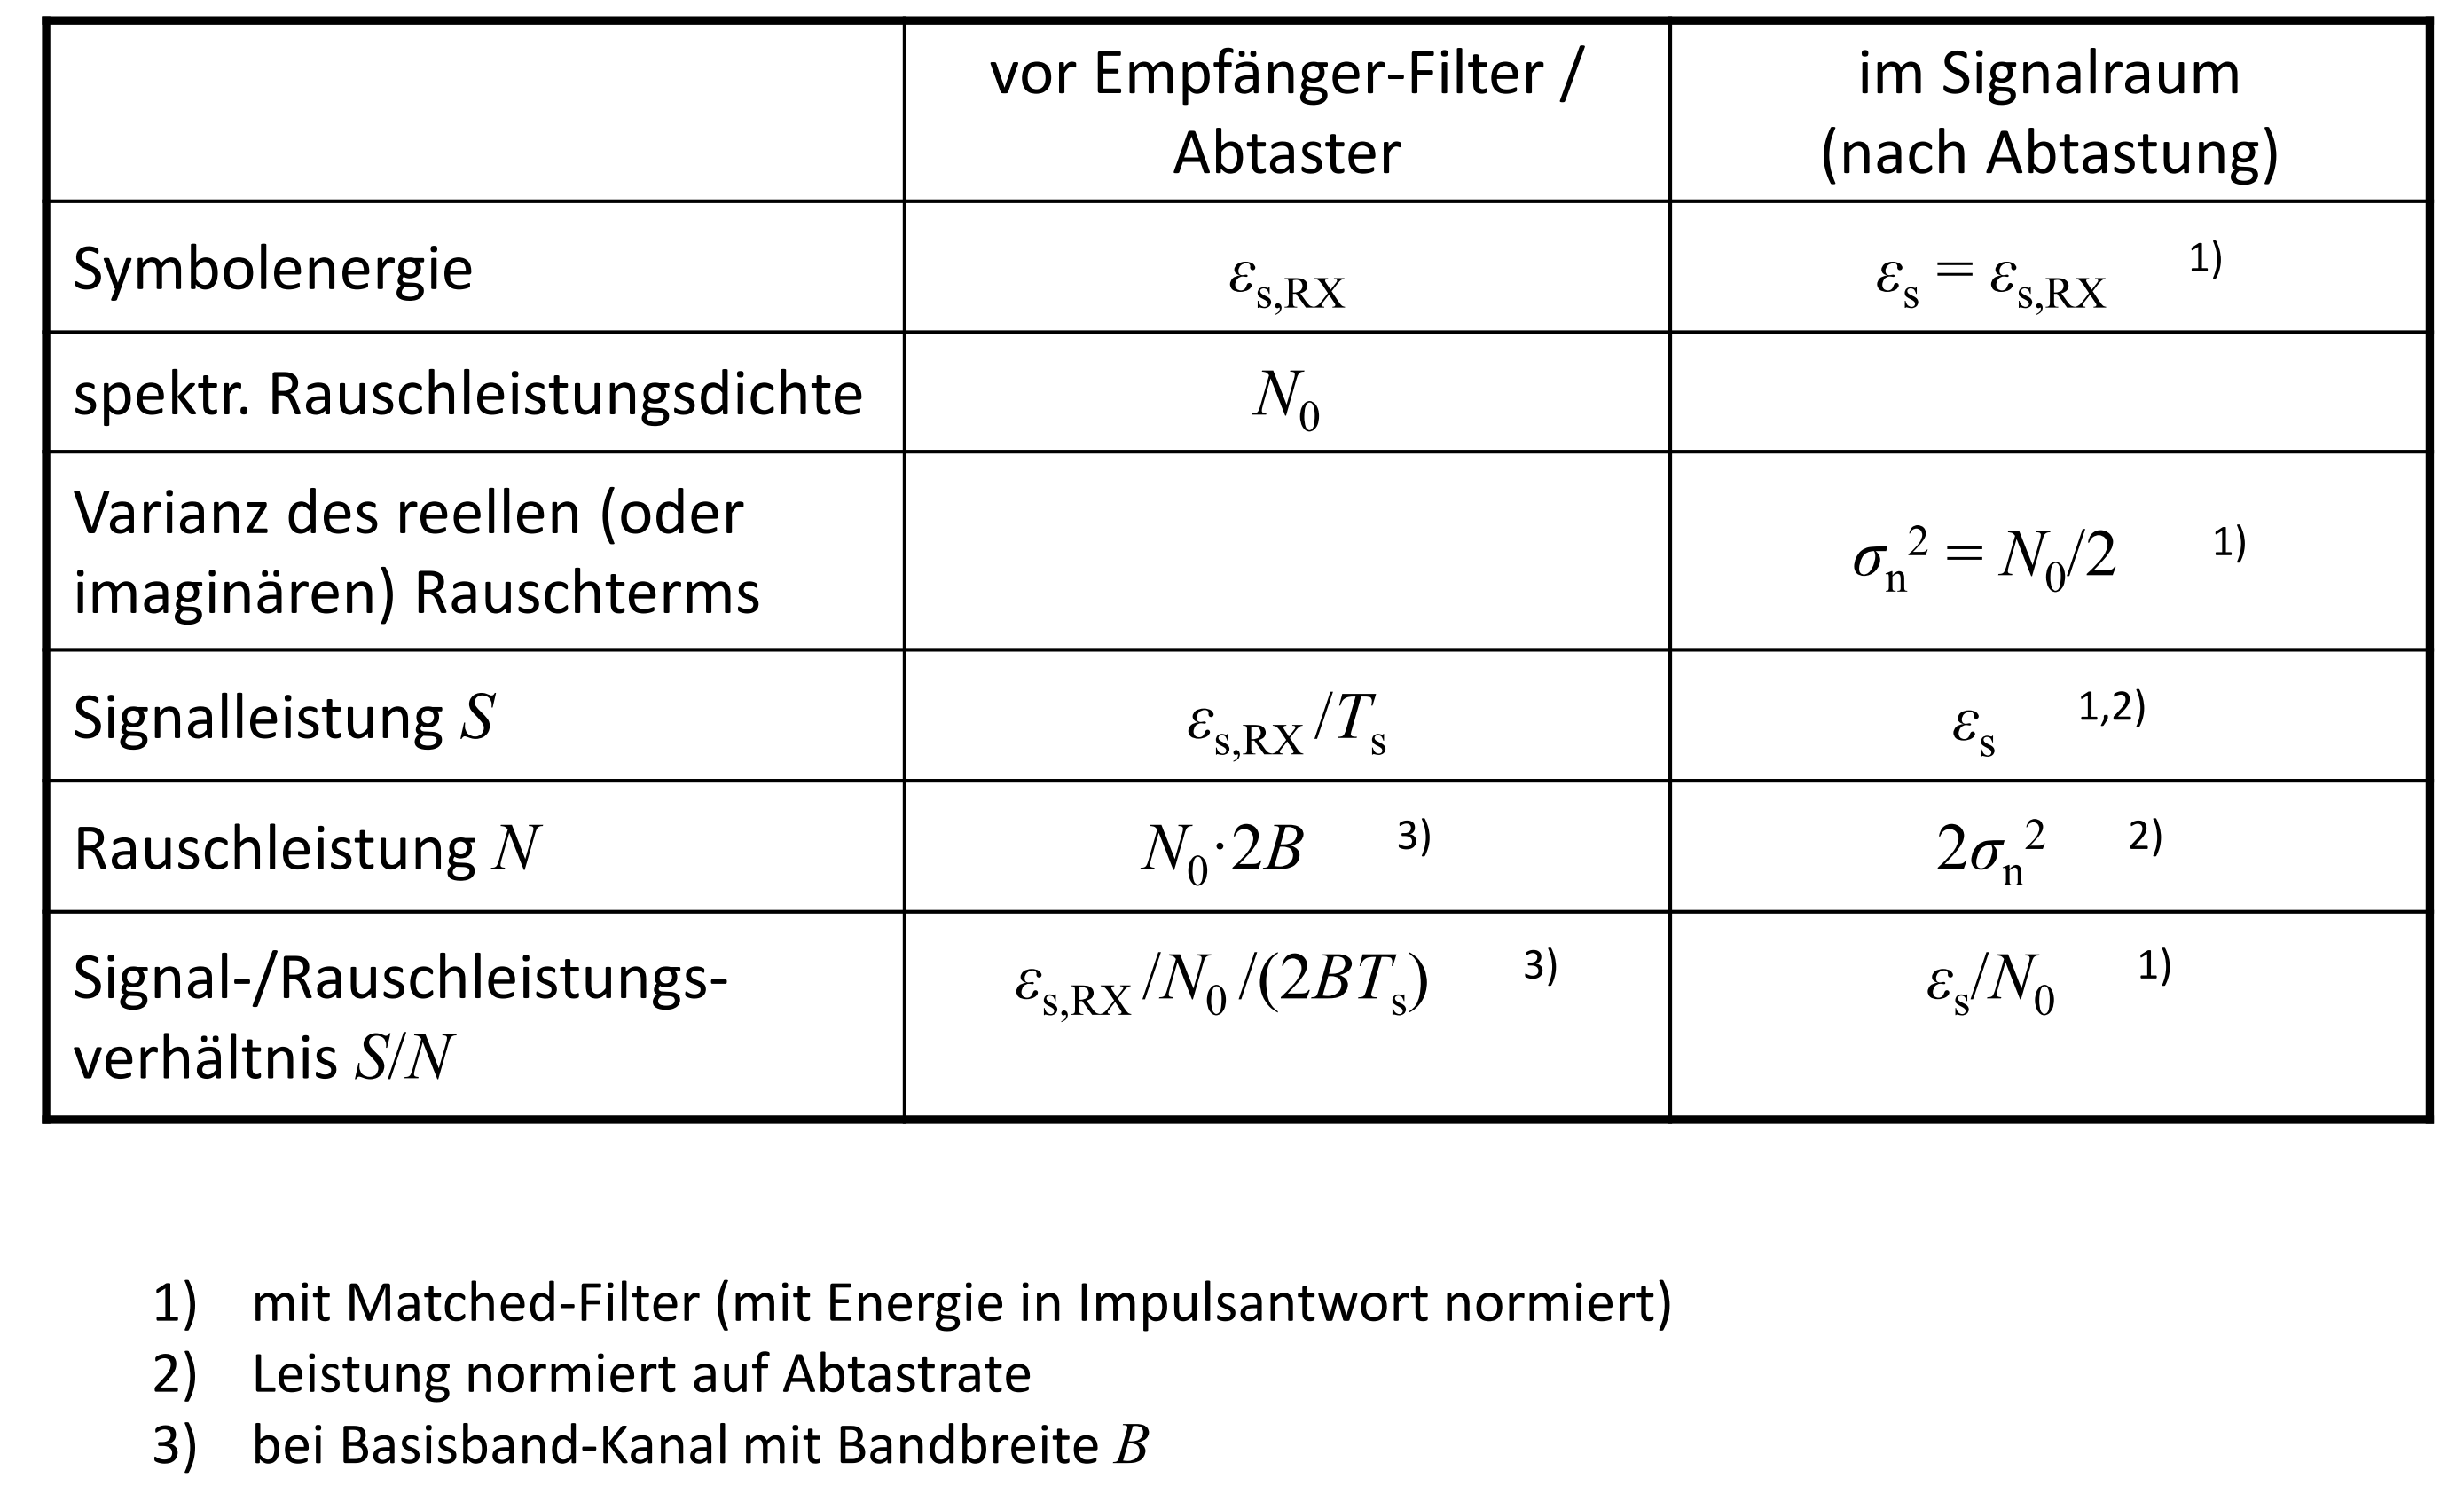
\includegraphics[width=.9\textwidth]{./images/snr.png}
\end{center}
\chapter{Impulsformung}
Leistungsdichtespektrum bei bipolarer Signalisierung mit rechteckfürmigen
Impulsen $p_{rect}(t)$ mit Rate $r_b=\frac{1}{T_b}$:

\begin{center}
	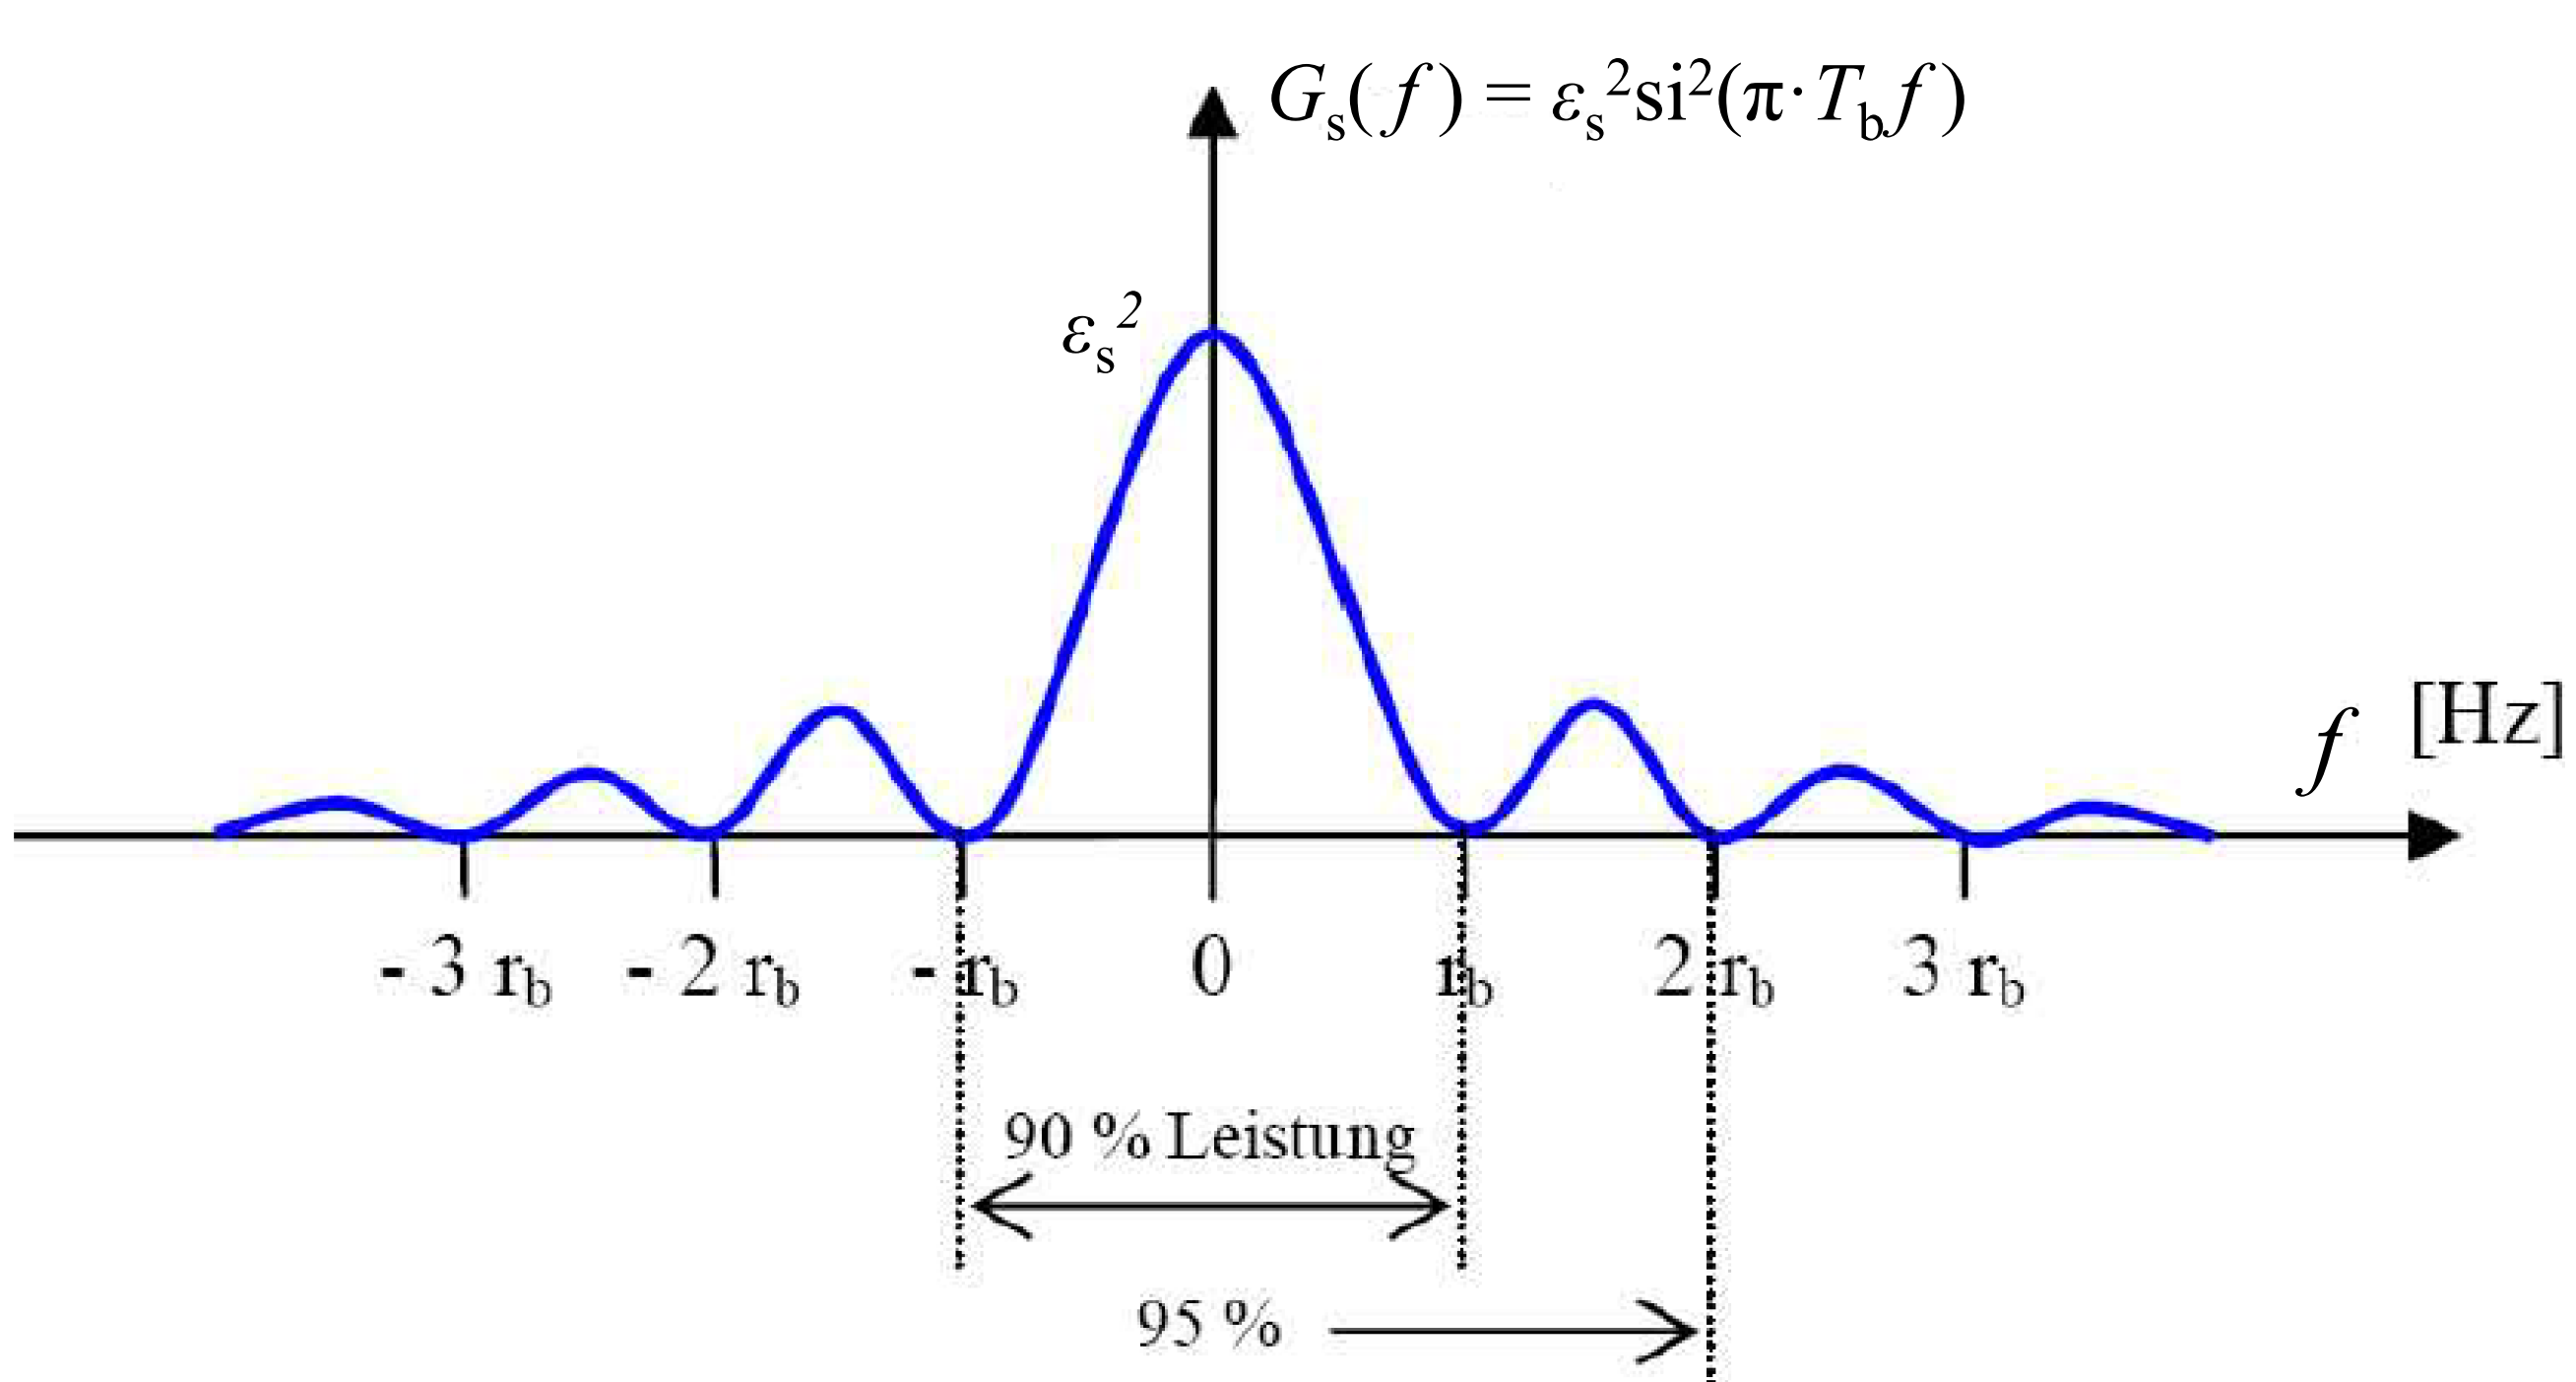
\includegraphics[width=.9\textwidth]{../fig/grect}
\end{center}
~\\
si-Impulse:
\[
	p_{si}(t) = T_b^{-\frac{1}{2}} \cdot \textrm{si}(\pi r_b t)
\]
\begin{center}
	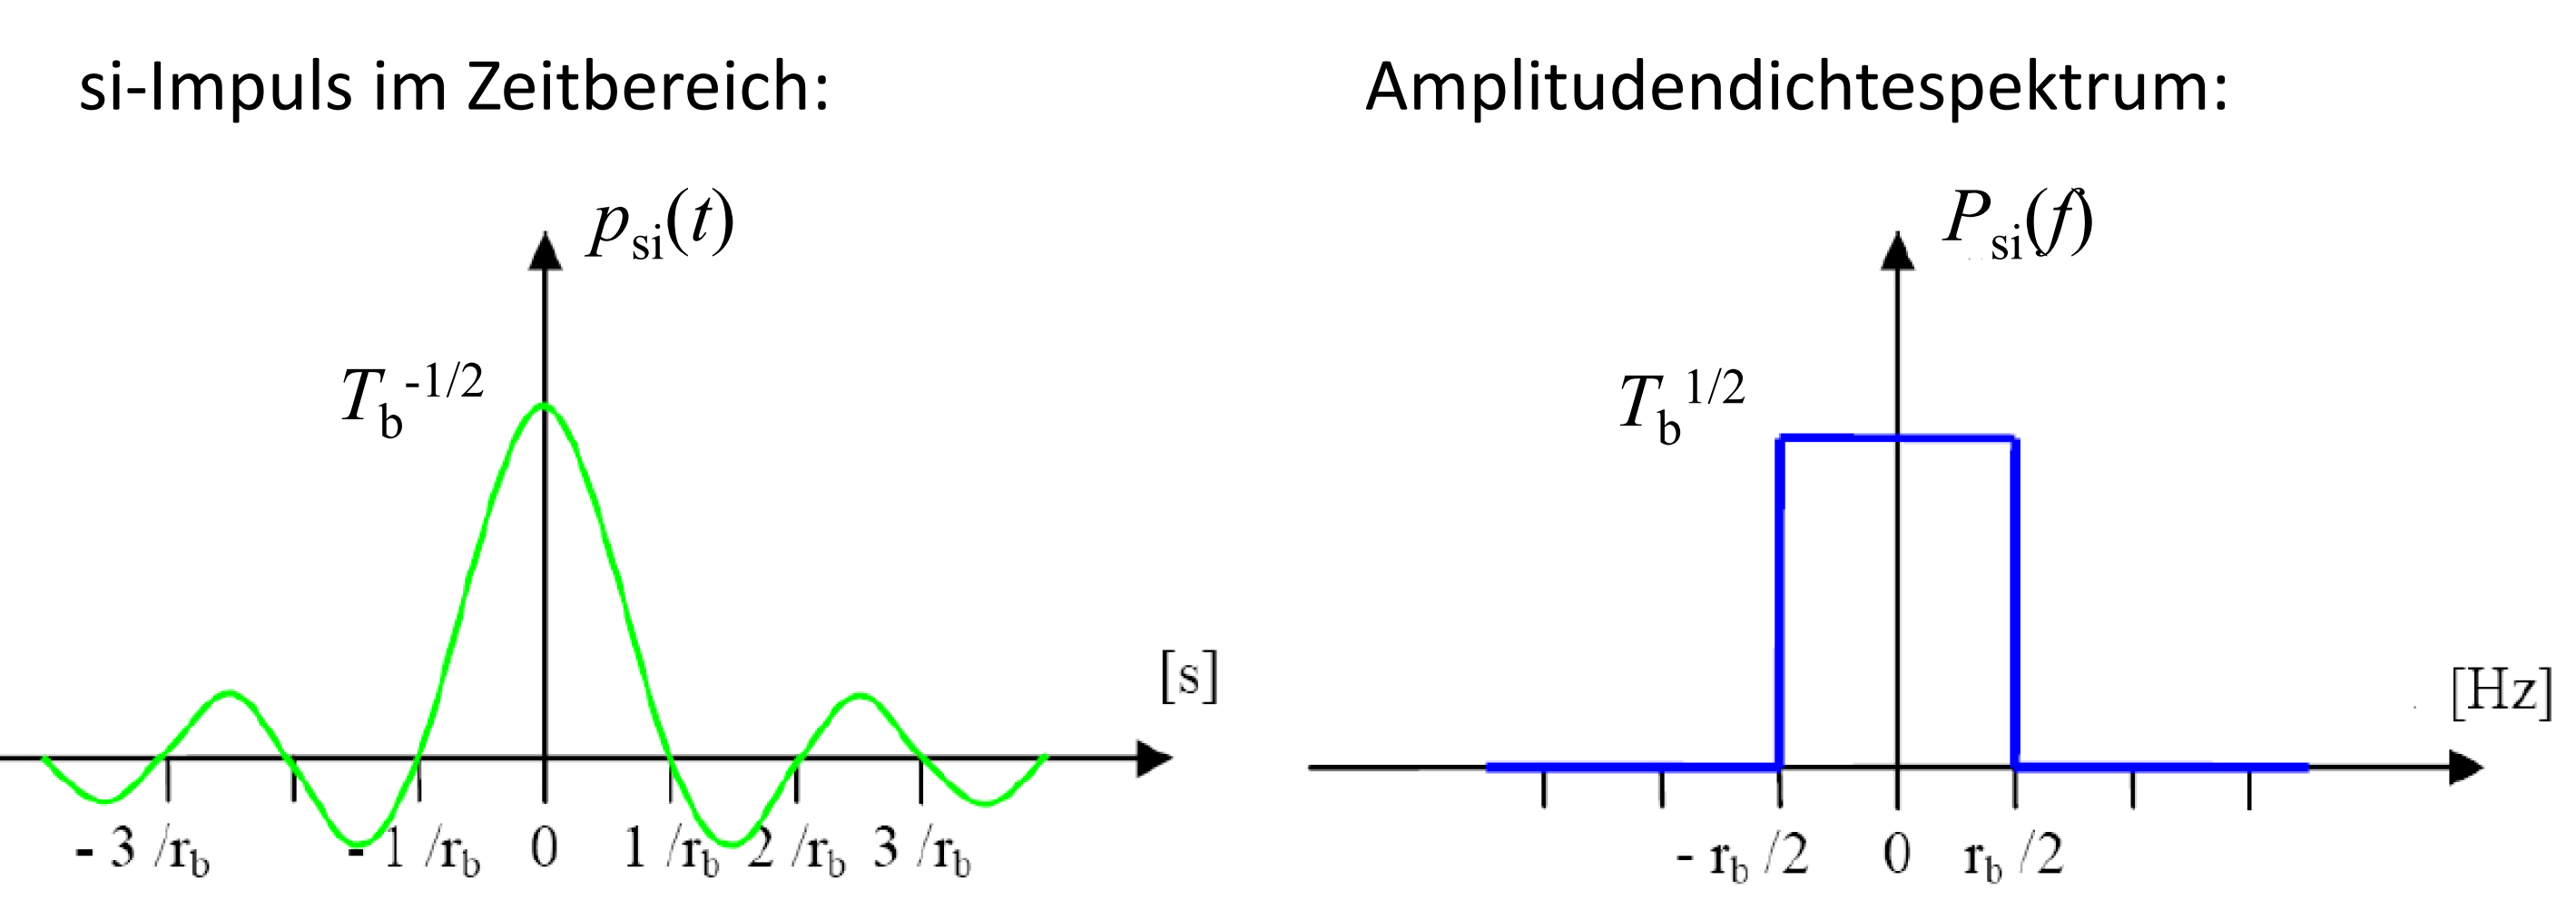
\includegraphics[width=.9\textwidth]{../fig/si}
\end{center}

\section{ISI-freie Detektion}
Eine Abtastung zu idealen Zeitpunkten ermöglicht eine ISI-freie Detetkion wenn:
\[\begin{aligned}
	p(0) &= A\\
	p(nT_b) &= 0 \qquad \textrm{, für } n=\pm1,\pm2,\ldots	
\end{aligned}\]
~\\Gemäss Nyquist erfüllt wenn:
\[
	\sum_{k=-\infty}^{\infty} P\left(f+\frac{k}{T_b}\right) = AT_b
\]

\section{raised-Cosine-Spectrum}
\[
	P_{rc}(f) = \left\lbrace
	\begin{matrix}
		AT_b & \textrm{, für } 0 \leq |f| \leq \frac{1-\alpha}{2T_b} \\
		\frac{AT_b}{2}\left(1 + \cos\left( \frac{\pi T_b}{\alpha}
			\left(|f|-\frac{1-\alpha}{2T_b} \right)\right)\right)
			& \textrm{, für } \frac{1-\alpha}{2T_b} \leq |f| \leq \frac{1+\alpha}{2T_b} \\
			0 & \textrm{, für } |f| > \frac{1+\alpha}{2T_b}
	\end{matrix}
	\right.
\]

\begin{center}
	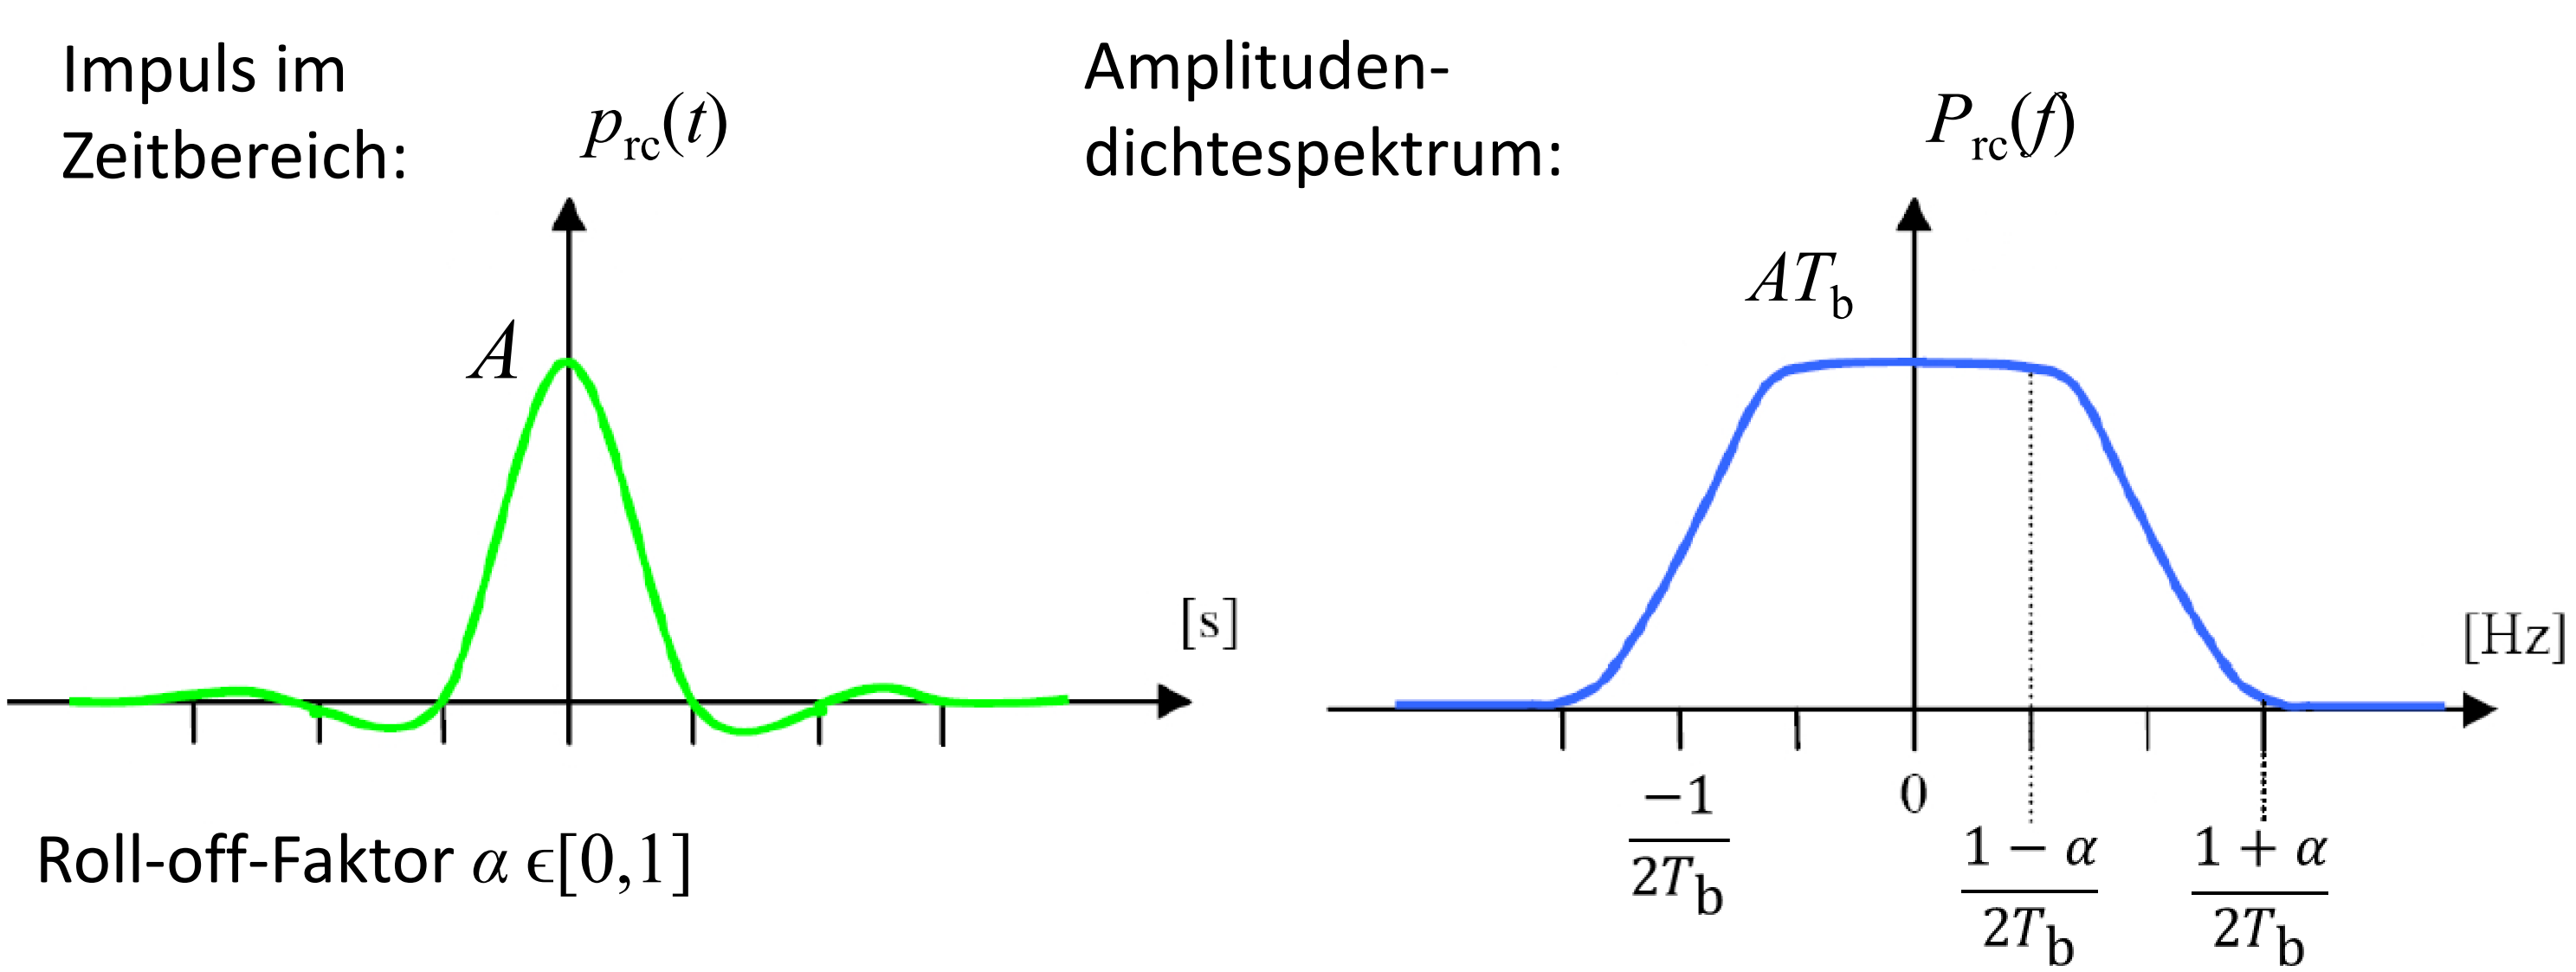
\includegraphics[width=.9\textwidth]{../fig/raisedcos.png}
\end{center}

\begin{center}
	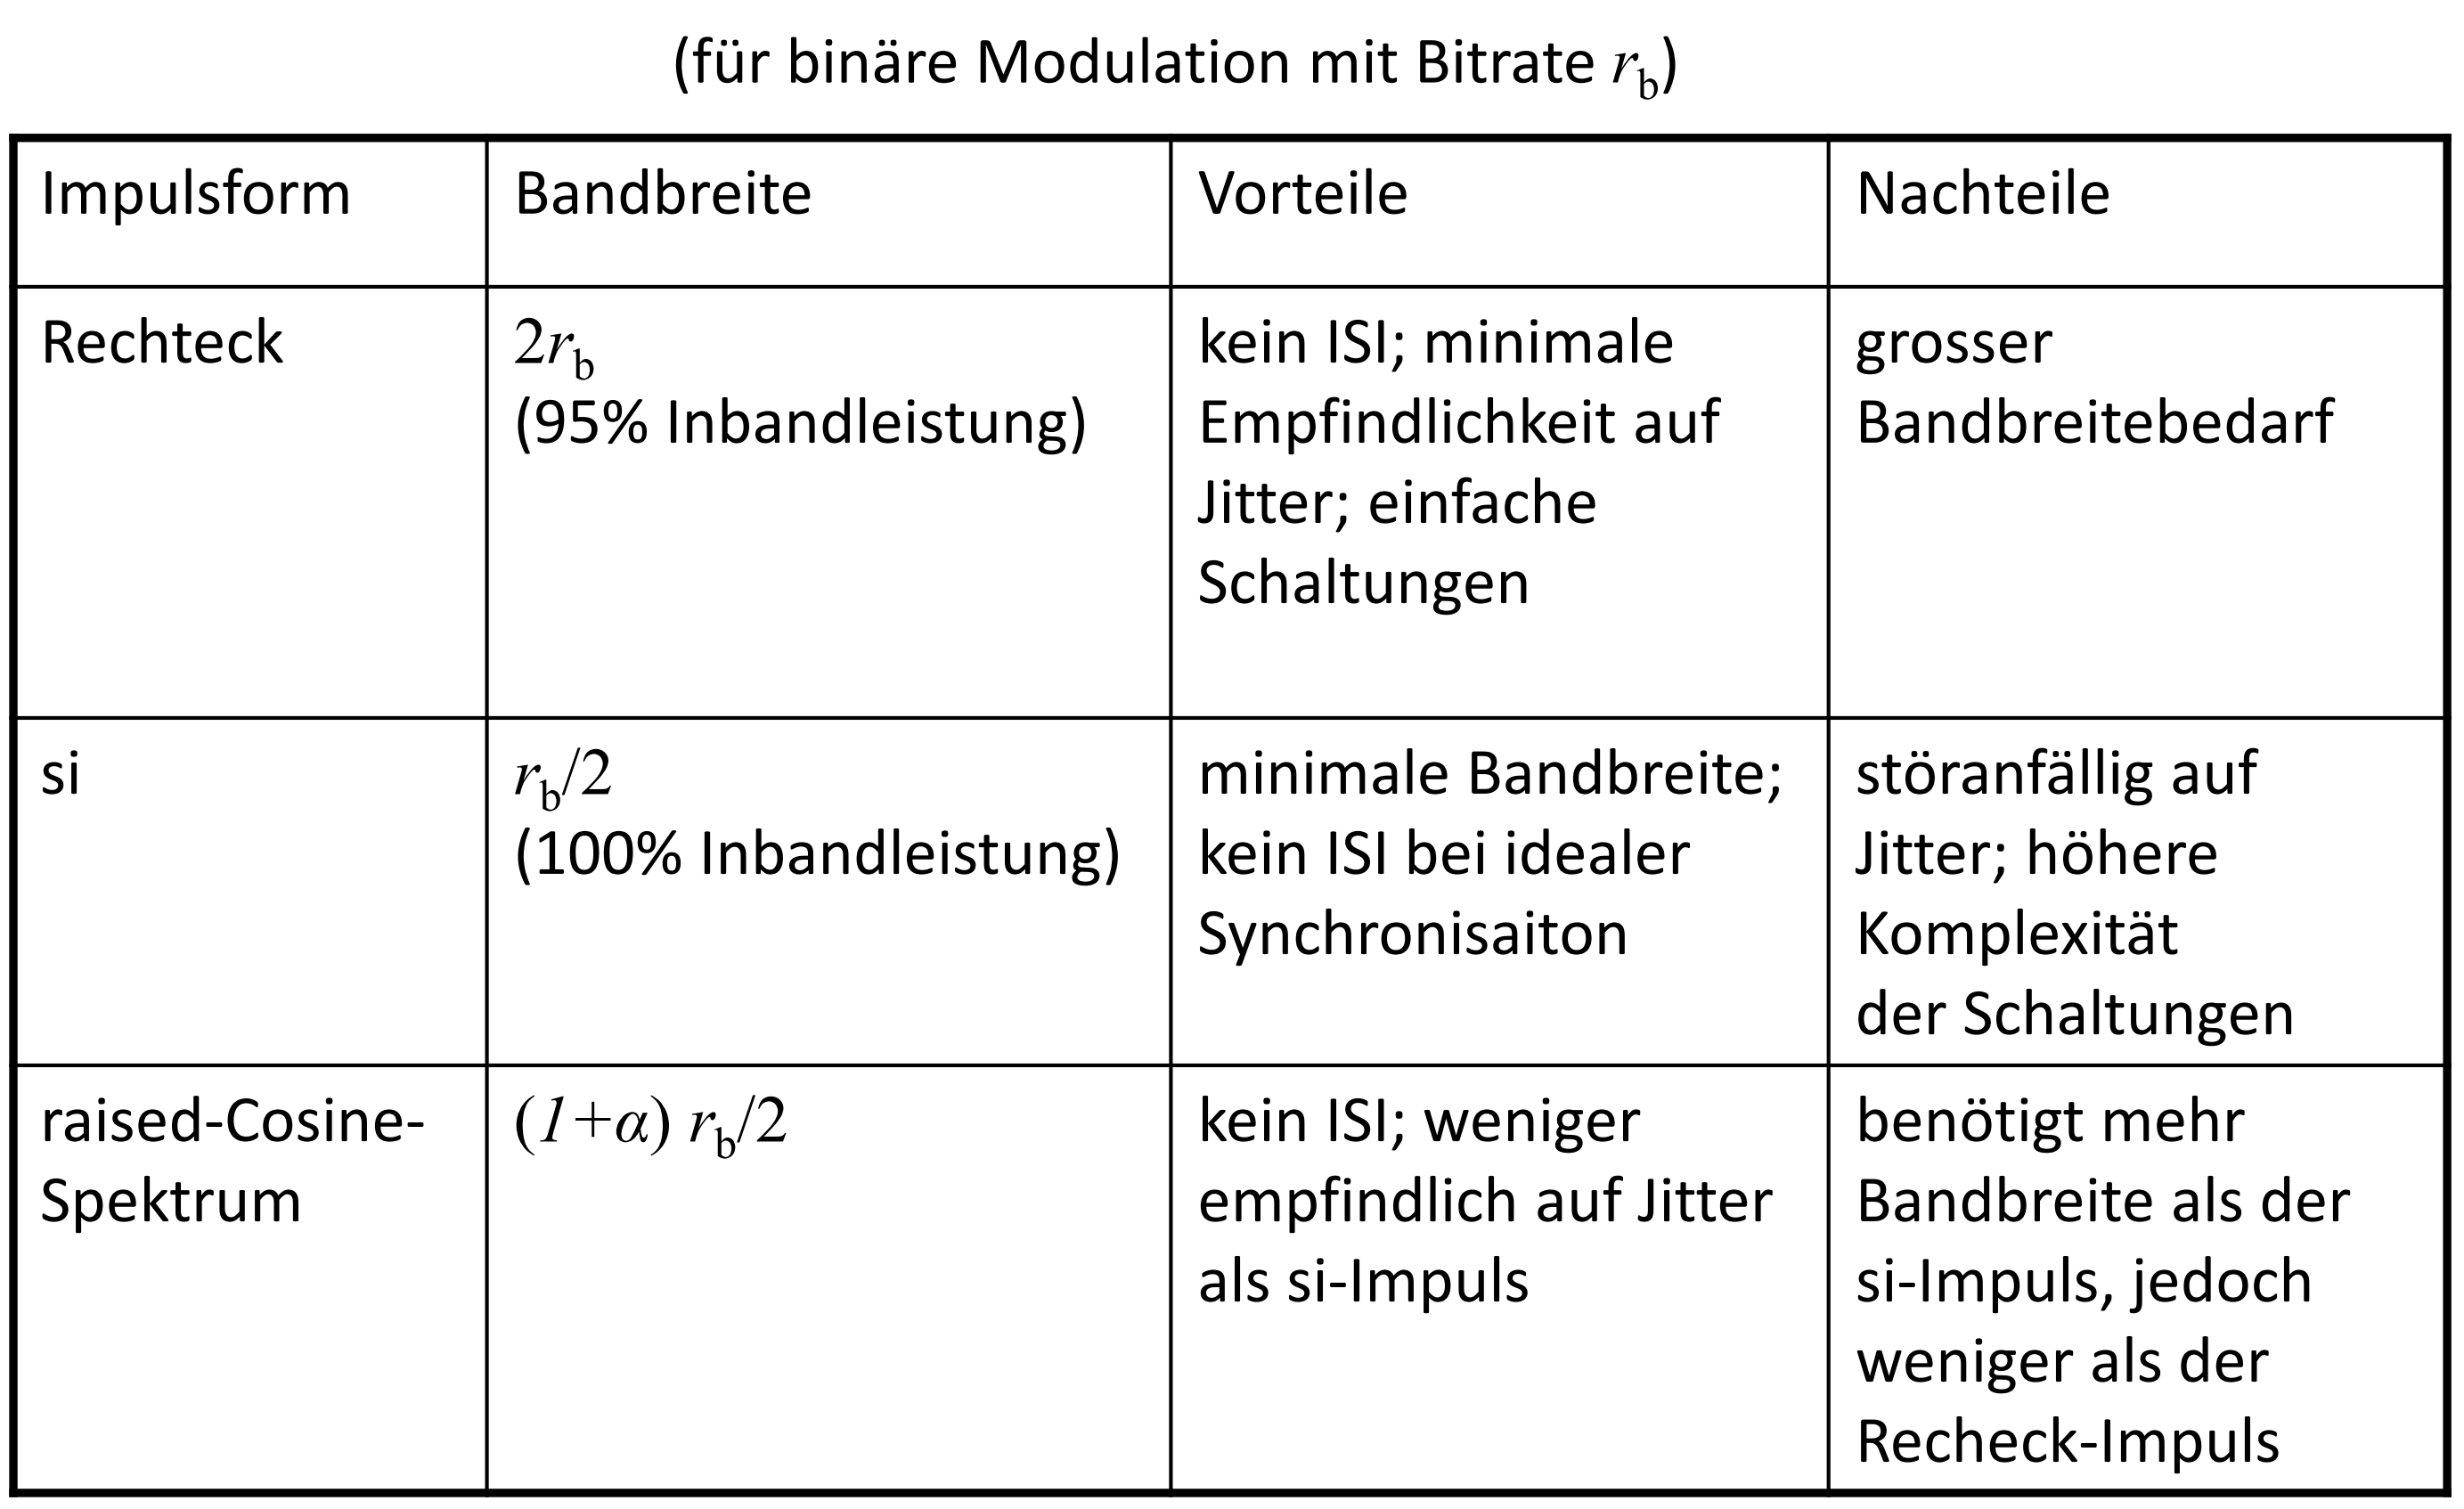
\includegraphics[width=.9\textwidth]{../fig/vergleich.png}
\end{center}

\chapter{Spreizcode}
\begin{itemize}
	\item Erhöhung der Robustheit bei Übertragung über frequenz-selektive Funkkanäle
	\item CDMA-Vielfachzugriff: Verfahren zur flexiblen Akkommodierung von Benutzern
	in Umgebungen mit zeitvarianten Auslastungen
\end{itemize}

\begin{center}
	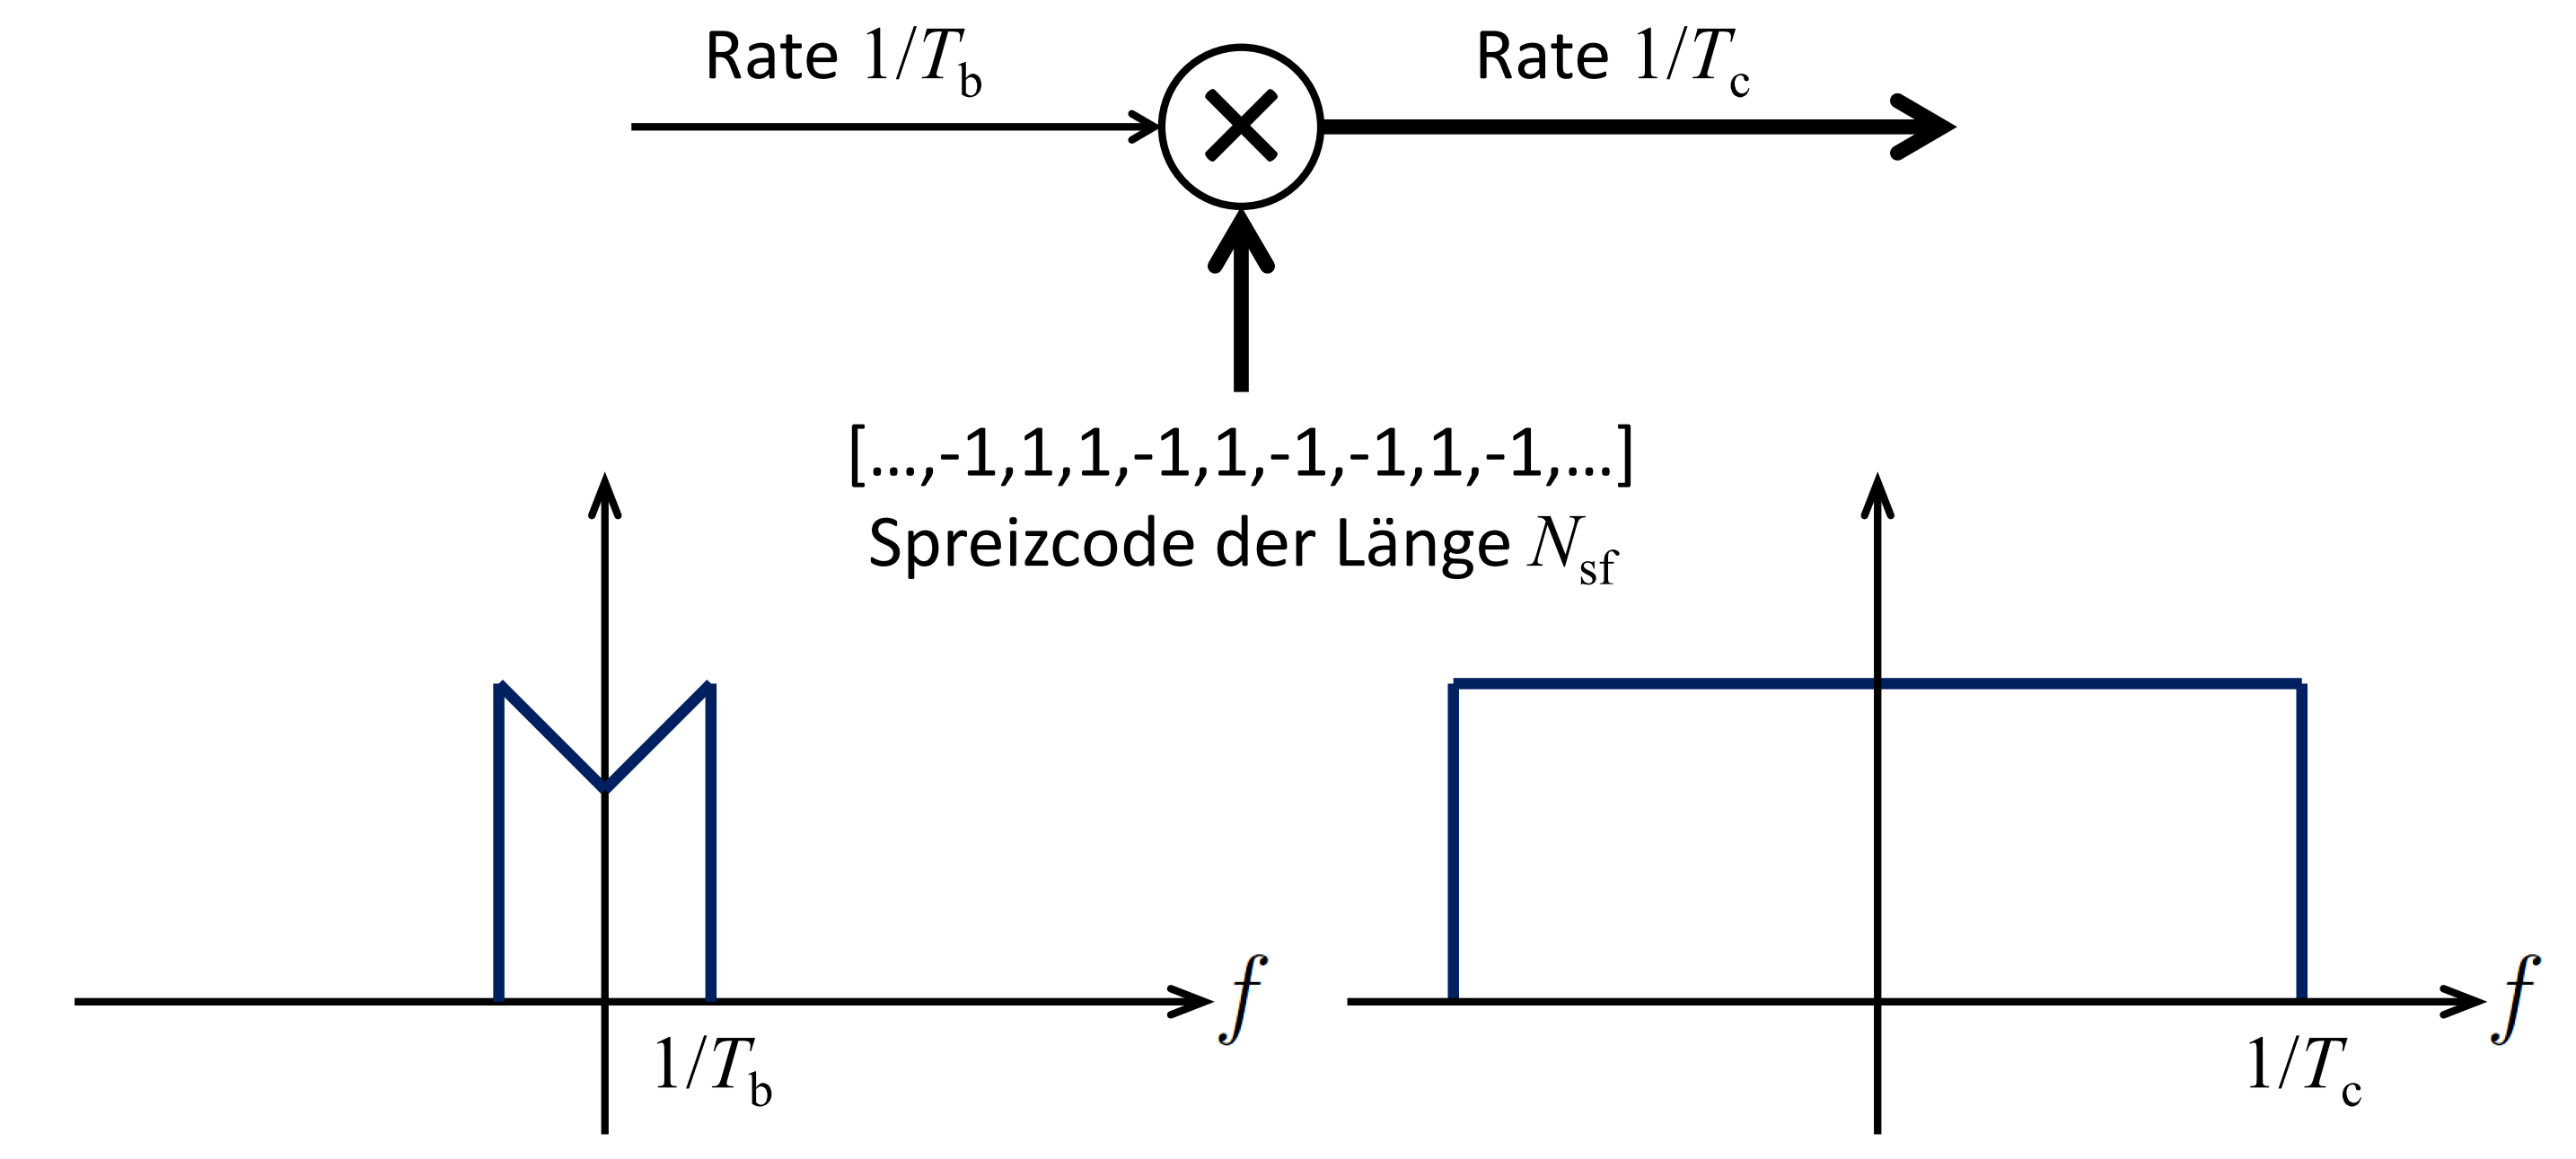
\includegraphics[width=.9\textwidth]{./images/spreiz.png}
\end{center}
~\\
Sprading Factor (Prozessgewinn):
\[ N_{sf} = \frac{T_b}{T_c} \]

\section{Rake-Empfänger}
\begin{center}
	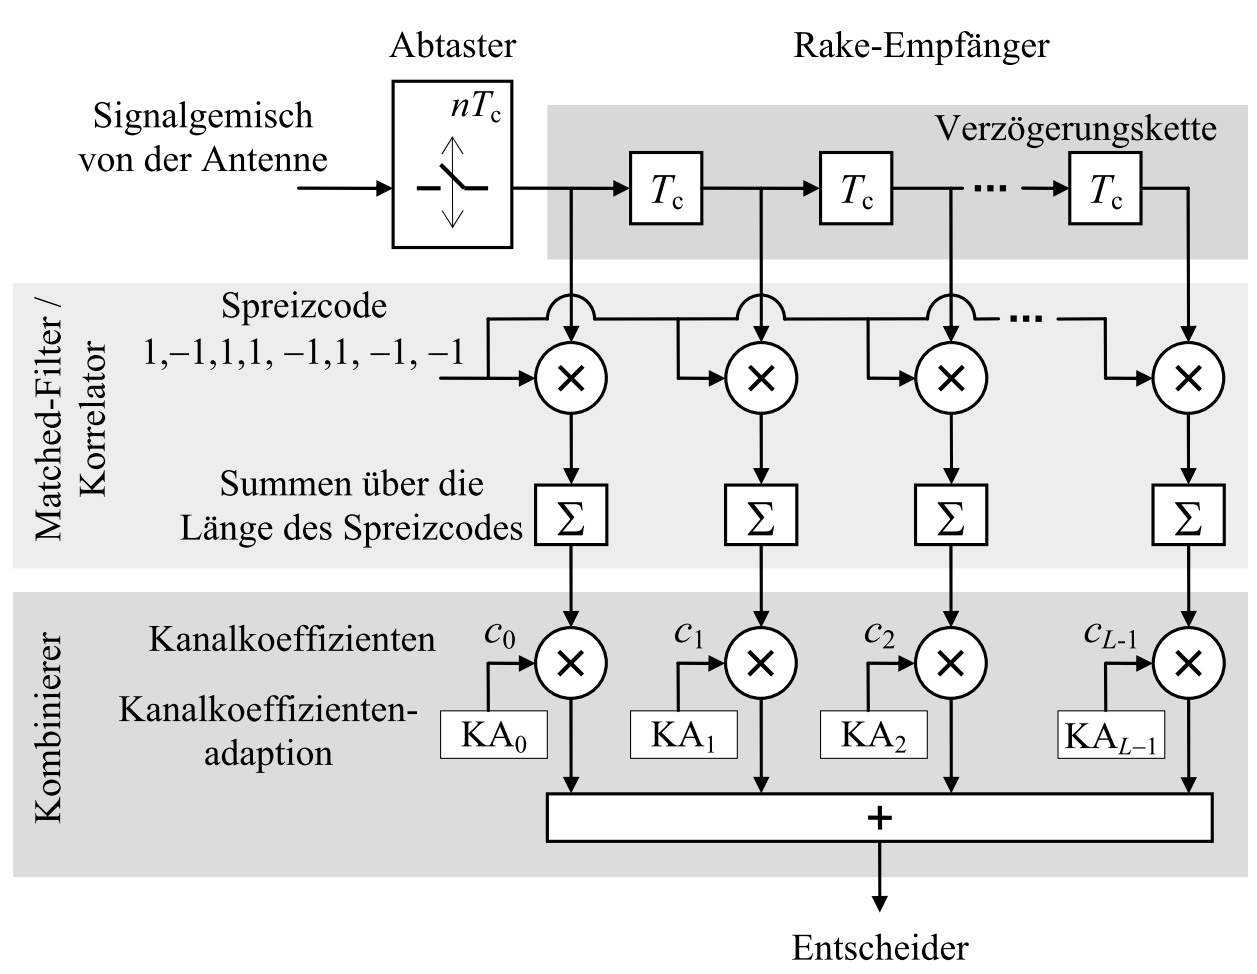
\includegraphics[width=.9\textwidth]{./images/rake.png}
\end{center}

\section{CDMA-Vielfachzugriff}
\begin{center}
	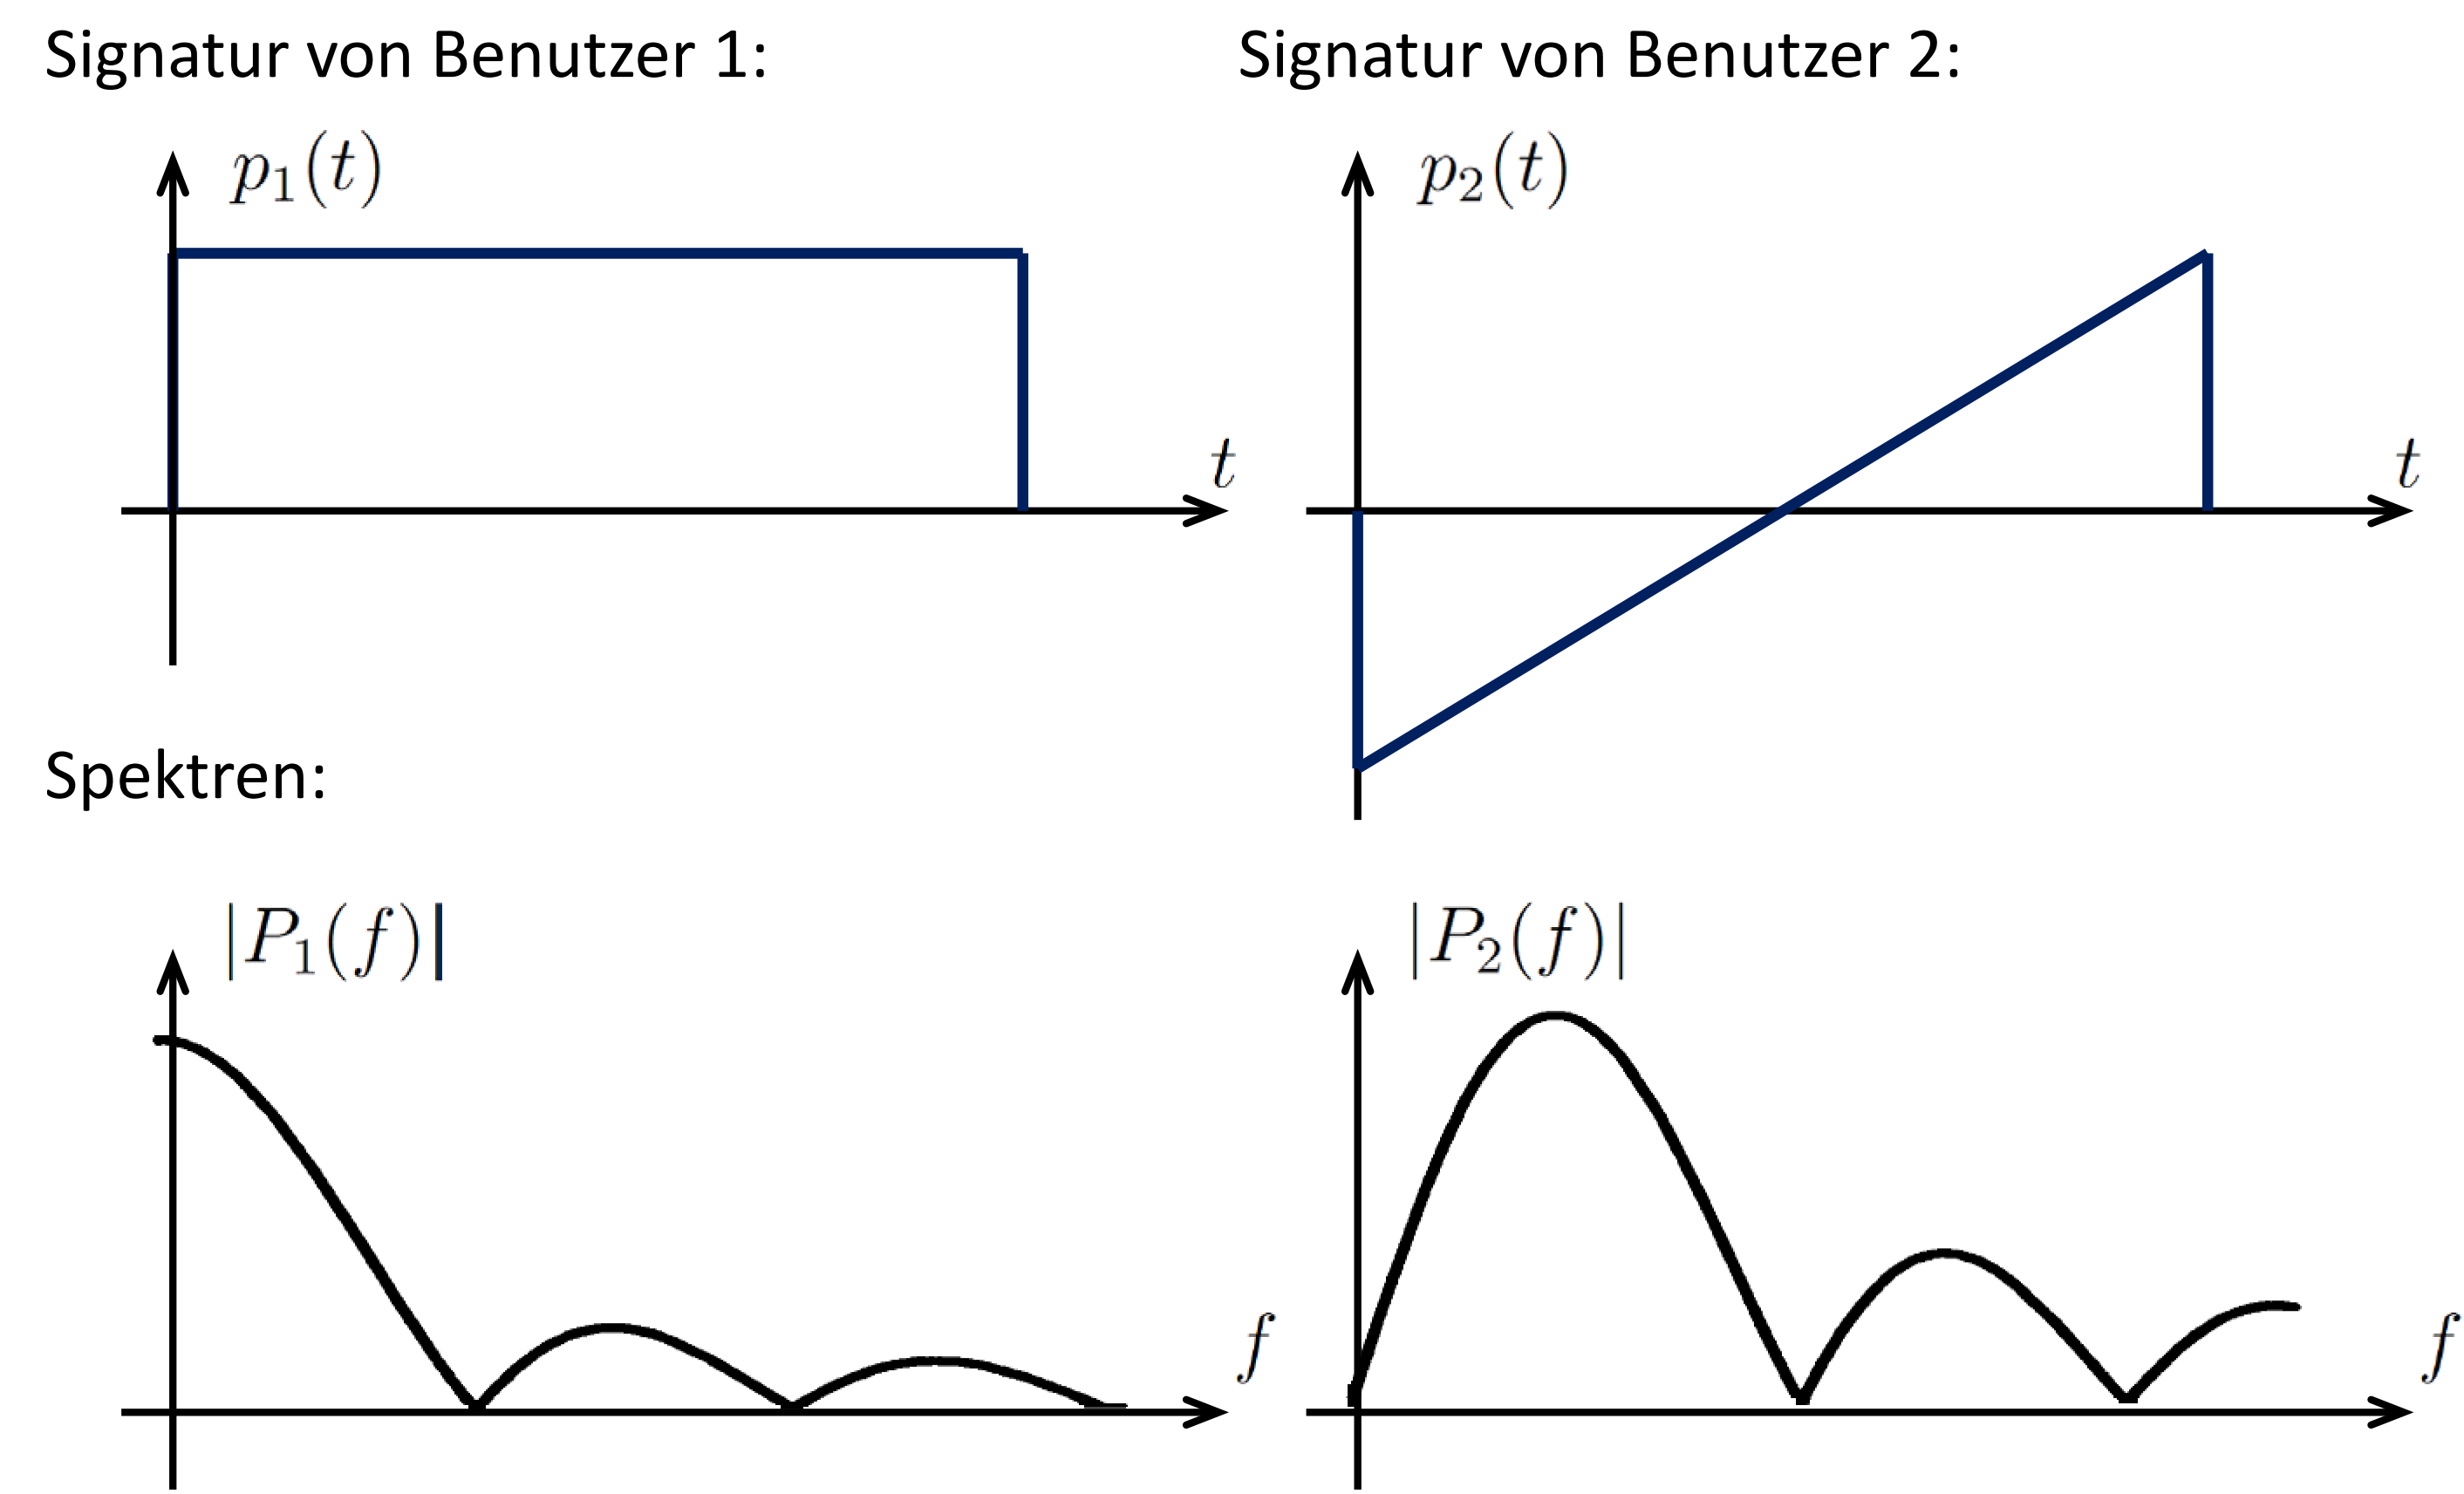
\includegraphics[width=.9\textwidth]{./images/cdma.png}
\end{center}

\section{OVSF Codes}
\begin{center}
	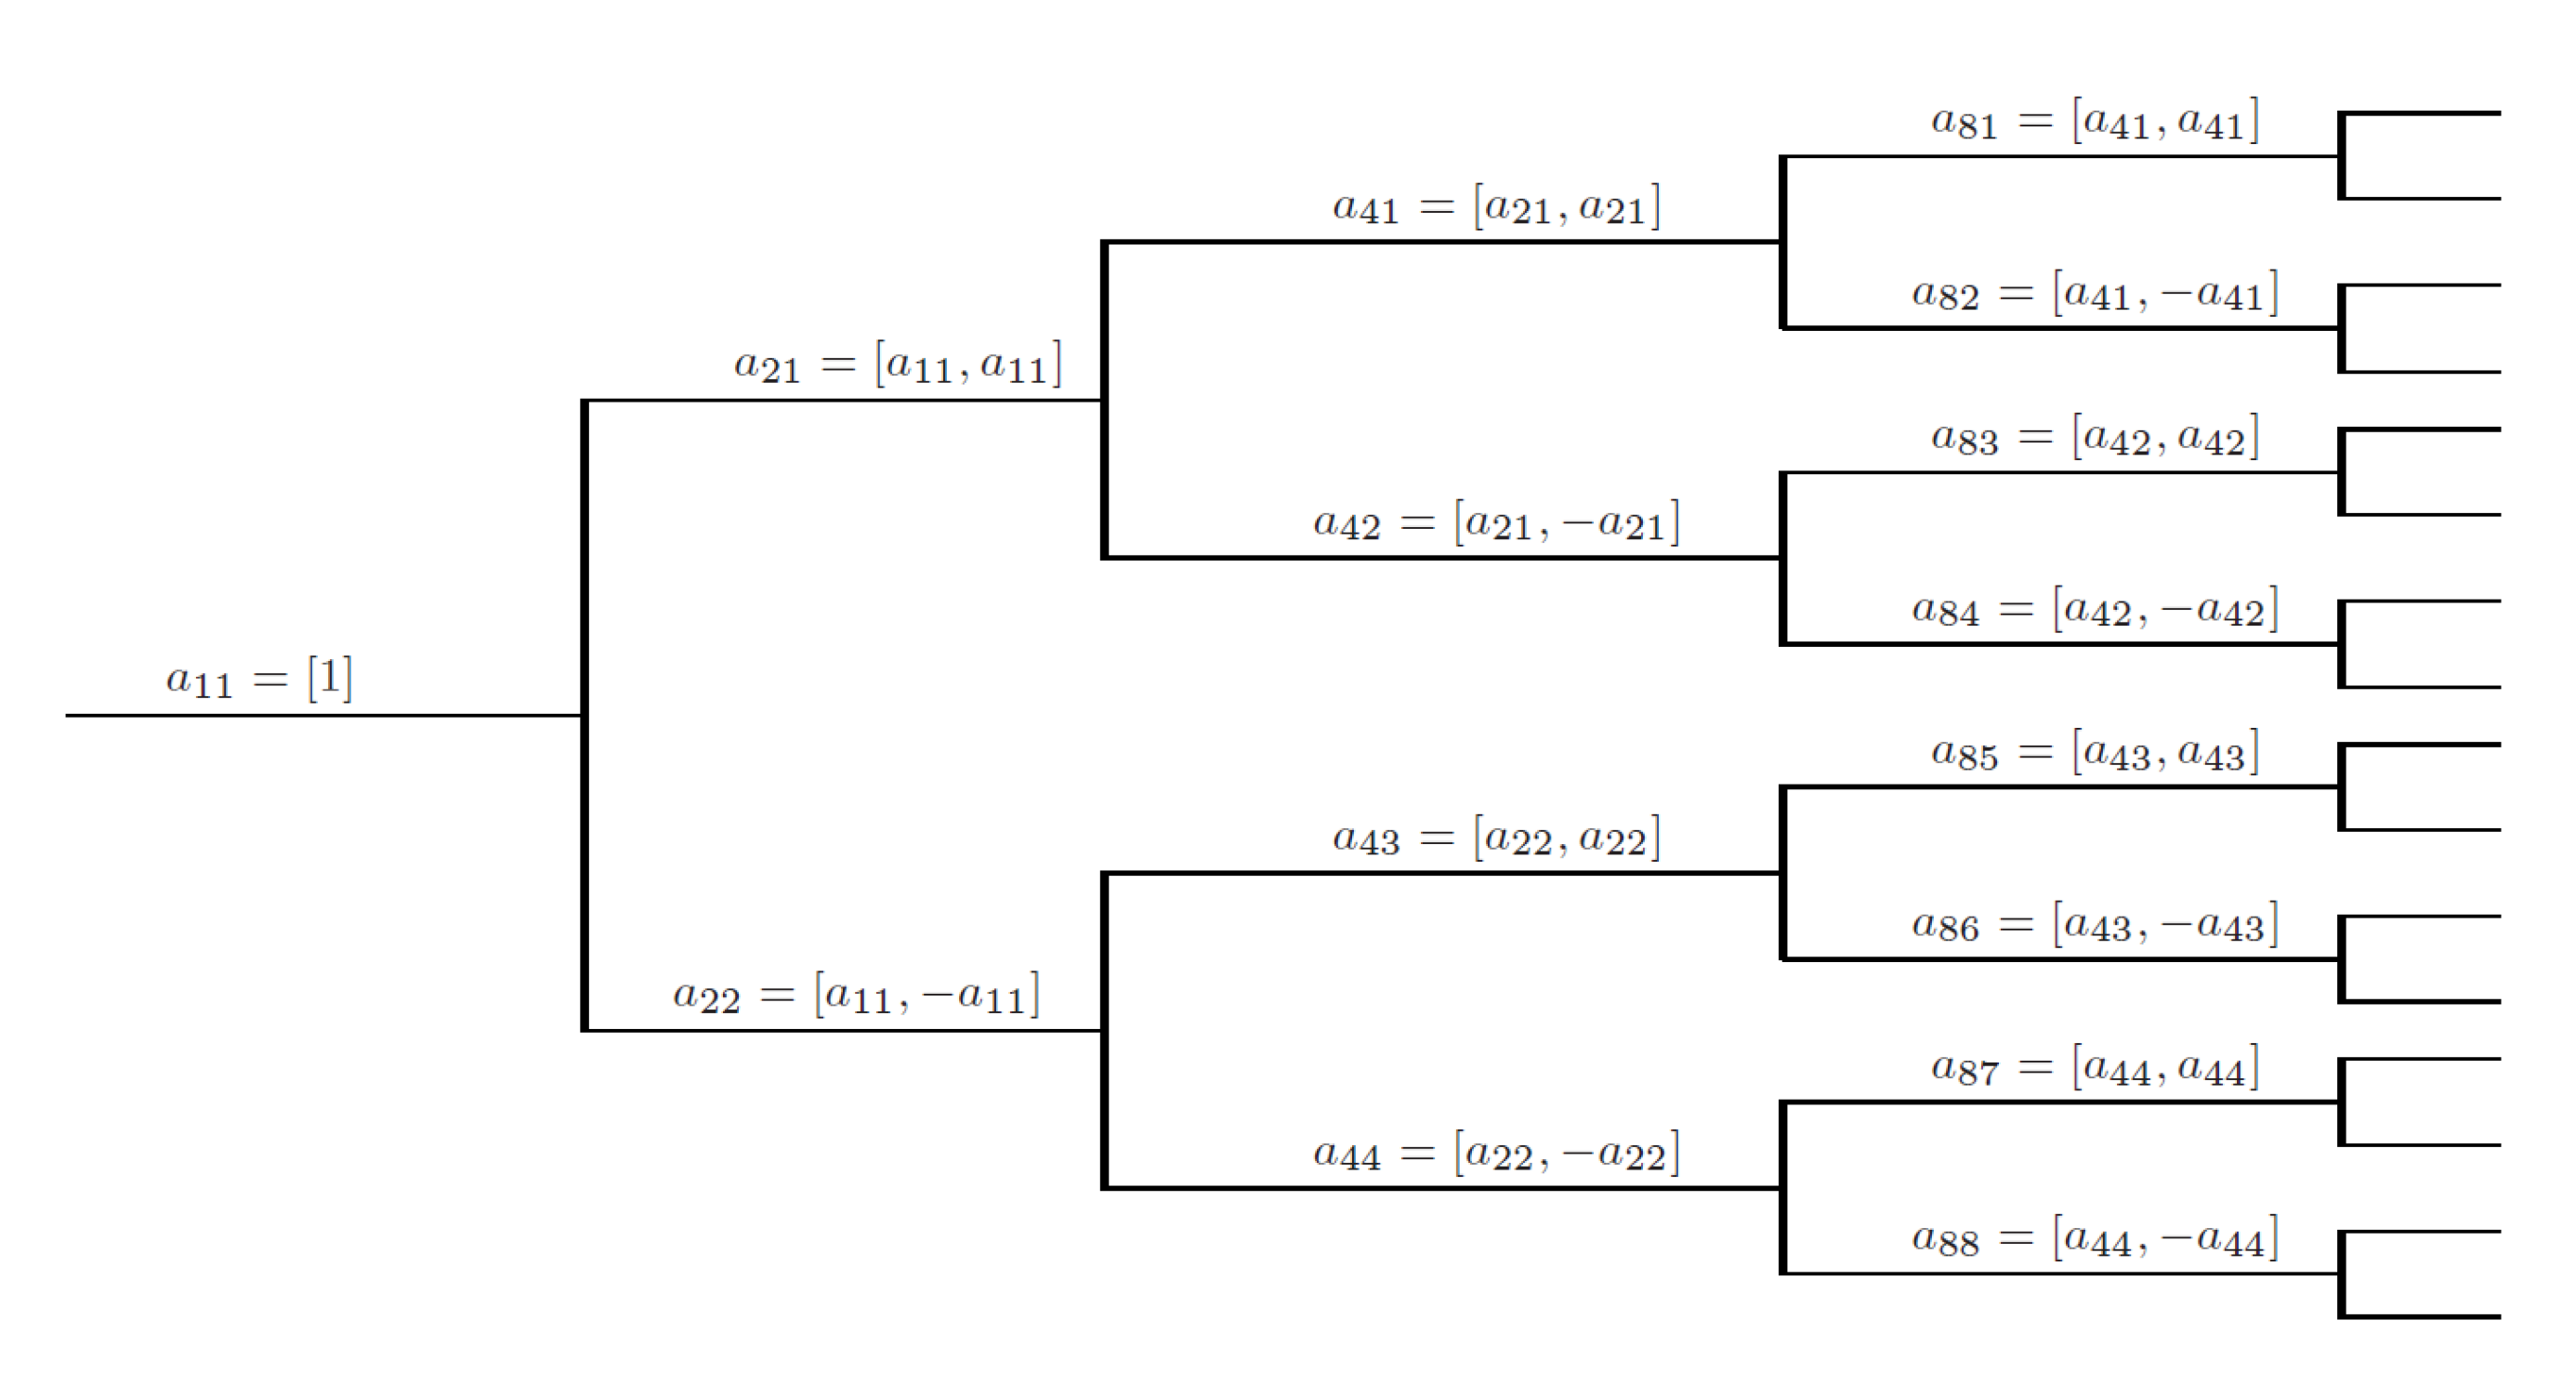
\includegraphics[width=.9\textwidth]{./images/ovsf.png}
\end{center}
\chapter{Informationsgehalt und Entropie}
gedächtnislose Quelle mit Alphabet $\Omega$.\\
diskrete Zufallsvariable $X$ mit Werten $\Omega = \lbrace x_1,\ldots,x_m \rbrace$.\\\\
Auftrittswahrscheinlichkeiten:
\[ P(X=x_i) = p(x_i) \qquad \sum_{i=1}^{M} = 1 \]
~\\Informationsgehalt des Symbols $x_i$:
\[ I(x_i) = -\log_2p(x_i) \textrm{ bit} \]
~\\Entropie von $X$: mittlere Information pro Symbol:
\[ H(X) = \sum_{i=1}^{M}p(x_i)I(x_i) = -\sum_{i=1}^{M}p(x_i)\log_2p(x_i) \textrm{ bit} \]

\section{Maximaler Entscheidungsgehalt und Redundanz}
Die Entropie einer diskreten gedächtnislosen Quelle wird maximal,
wenn alle $M$ Symbole des Symbolvorrats gleich wahrscheinlich sind,
wenn also $p(x_i)=\frac{1}{M}$:
\[ H(X) = \log_2M \textrm{ bit} \]
~\\$H(X)$ kann als maximalen Entscheidungsgehalt eines aus $M$ Symbolen bestehenden
Symbolvorrats betrachtet werden.\\\\
Für eine beliebige Quelle gilt ($R$ = Redundanz der Quelle):
\[ R = \log_2M-H(X) \geq 0 \]

\section{Codierung}
natürliche Codierung:
\\Codewörter der Länge $n$, wobei $\log_2M \leq n < \log_2M+1$
\\\\
Quellencodierungstheorem (Shannon):
\\für jedes $\varepsilon > 0$ gibt es einen binären Präfix-Code mit Bitrate
\[ r_b \leq r_s \cdot H(X) + \varepsilon \]

\subsection{Huffman-Codierung}
\begin{enumerate}
	\item Ordnen: Zeichen nach fallenden Wahrscheinlichkeiten ordnen
	\item Reduzieren: Zeichen mit den zwei kleinsten WSK zusammenfassen,
		wieder zu 1.
	\item Codieren: Starten bei letzter Zusammenfassung; jeweils eine
		0 dem oberen Zweig, eine 1 dem unteren.
\end{enumerate}
\begin{center}
	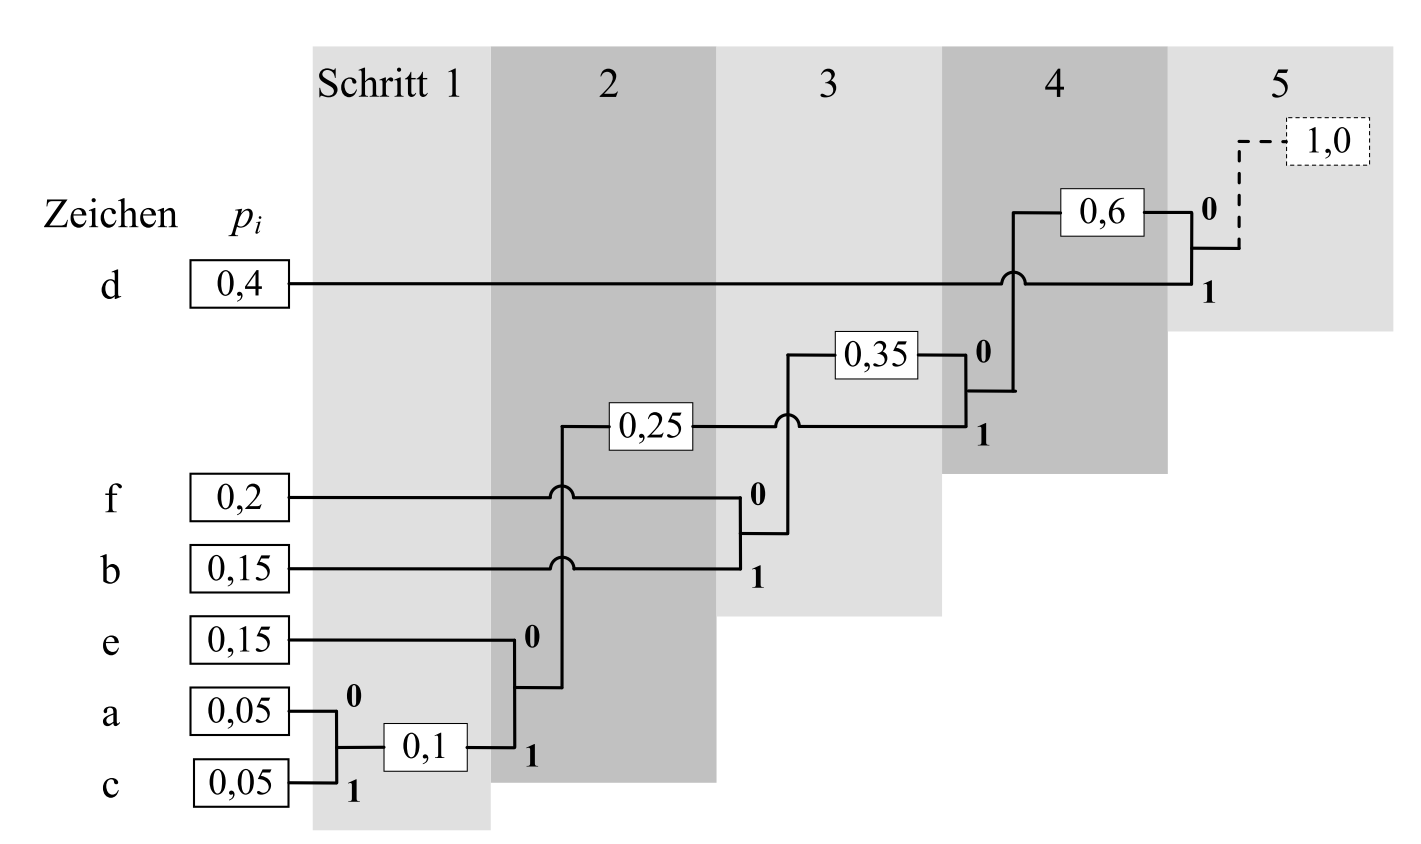
\includegraphics[width=.9\textwidth]{../fig/huffman.png}
\end{center}
~\\
mittlere Codewortlänge:
\[ \bar{n} = \sum_{i=1}^{N}p_i \cdot n_i \]
~\\
Effizienz des Codes:
\[ \eta = \frac{H(X)}{\bar{n}} \]

\section{Bedingte Wahrscheinlichkeit}
Wahrscheinlichkeit von $y$ gegeben $x$:
\[ p(y|x) = \frac{p(x,y)}{p(x)} \]
~\\
Bedingter Informationsgehalt:
\[ I(y_j|x_i) = -\log_2p(y_j|x_i) \]
~\\
Wechselseitige Information des Symbolpaars ($x_i$,$y_j$) (Verbundquelle):
\[ I(x_i;y_j) = \log_2\frac{p(y_j|x_i)}{p(y_j)} = \log_2\frac{p(x_i|y_j)}{p(x_i)} \]
~\\
Informationsgehalt eines Symbolpaars:
\[ I(x_i,y_j) = I(x_i) + I(y_j) - I(x_i;y_j) \]
\[ I(x_i,y_j) = I(x_i) + I(y_j|x_i)  \]

\section{Verbundquellen}
Verbundentropie:
\[ H(X,Y) = - \sum_{i=1}^{M}\sum_{j=1}^{N} p(x_i,y_j)\log_2p(x_i,y_j) \]
~\\
bedingte Entropie:
\[ H(Y|X) = - \sum_{i=1}^{M}\sum_{j=1}^{N} p(x_i,y_j)\log_2p(x_i|y_j) \]

\begin{center}
	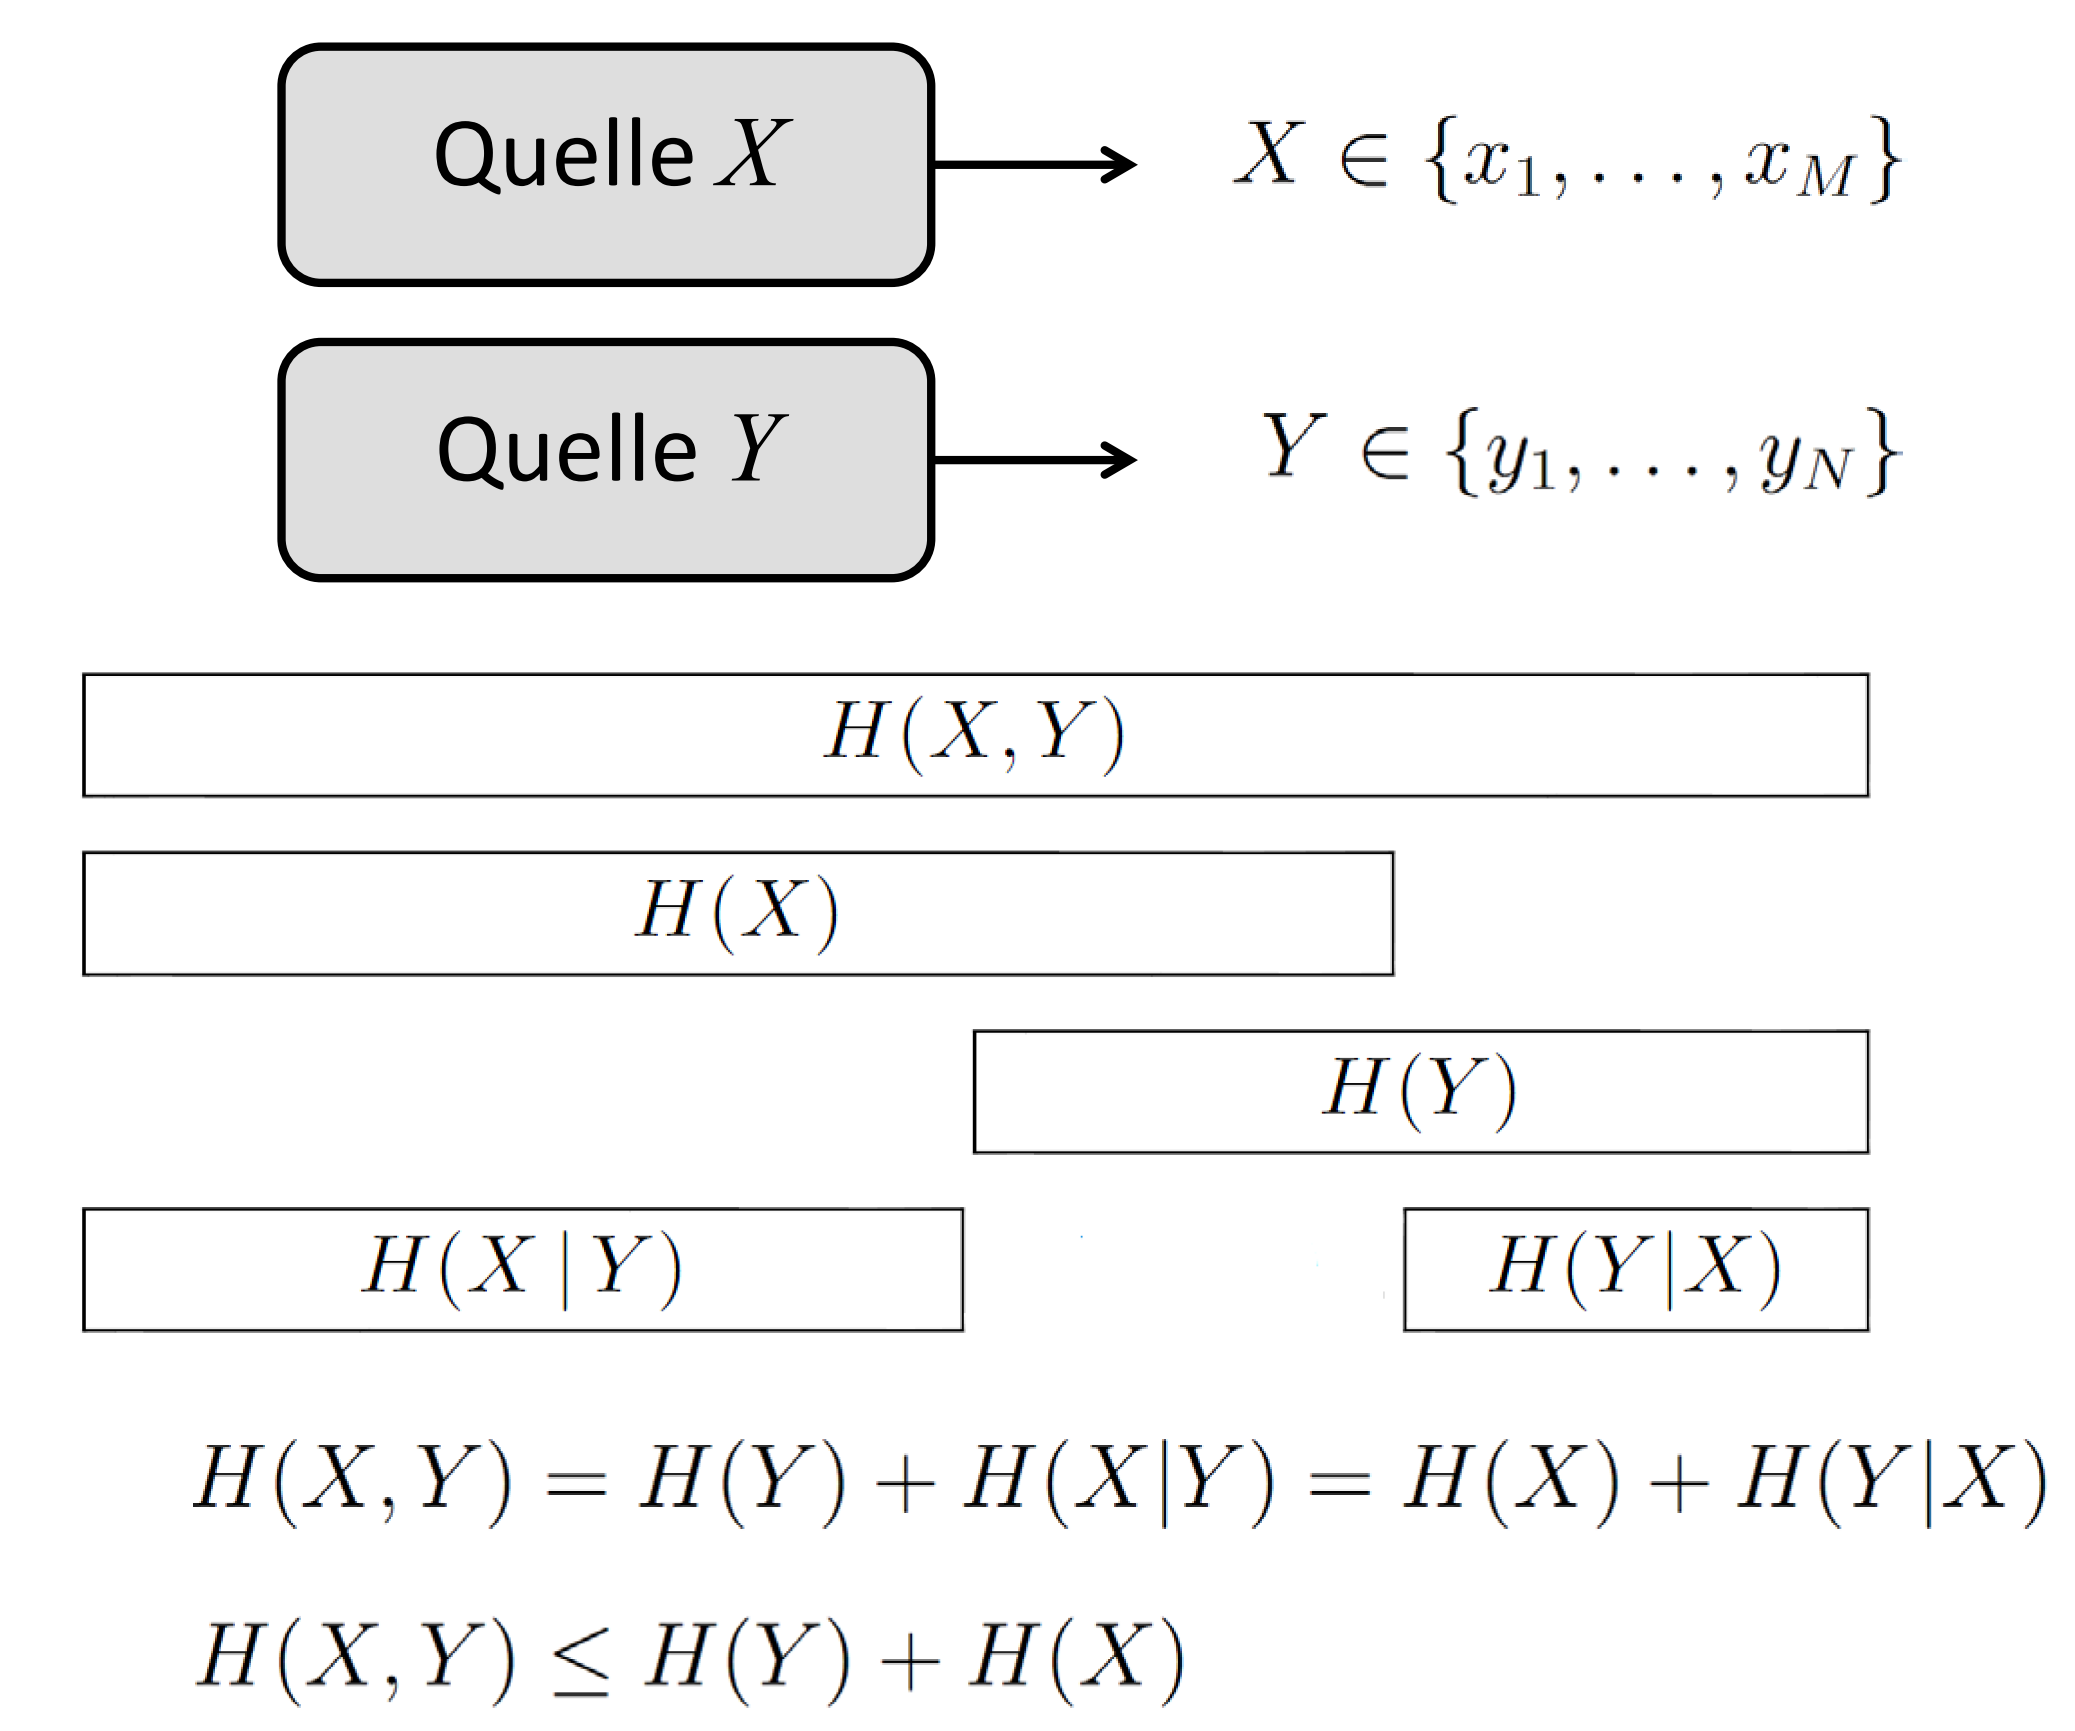
\includegraphics[width=.9\textwidth]{../fig/verbundentro.png}
\end{center}

\section{Transinformation}
Transinfomration (mutual information):
\[ I(X;Y) = \sum_{i=1}^{M}\sum_{j=1}^{N}p(x_i,y_j)\log_2\frac{p(y_j|x_i)}{p(y_j)}
	= \sum_{i=1}^{M}\sum_{j=1}^{N}p(x_i,y_j)\log_2\frac{p(x_i|y_j)}{p(x_i)} \]
	
\begin{center}
	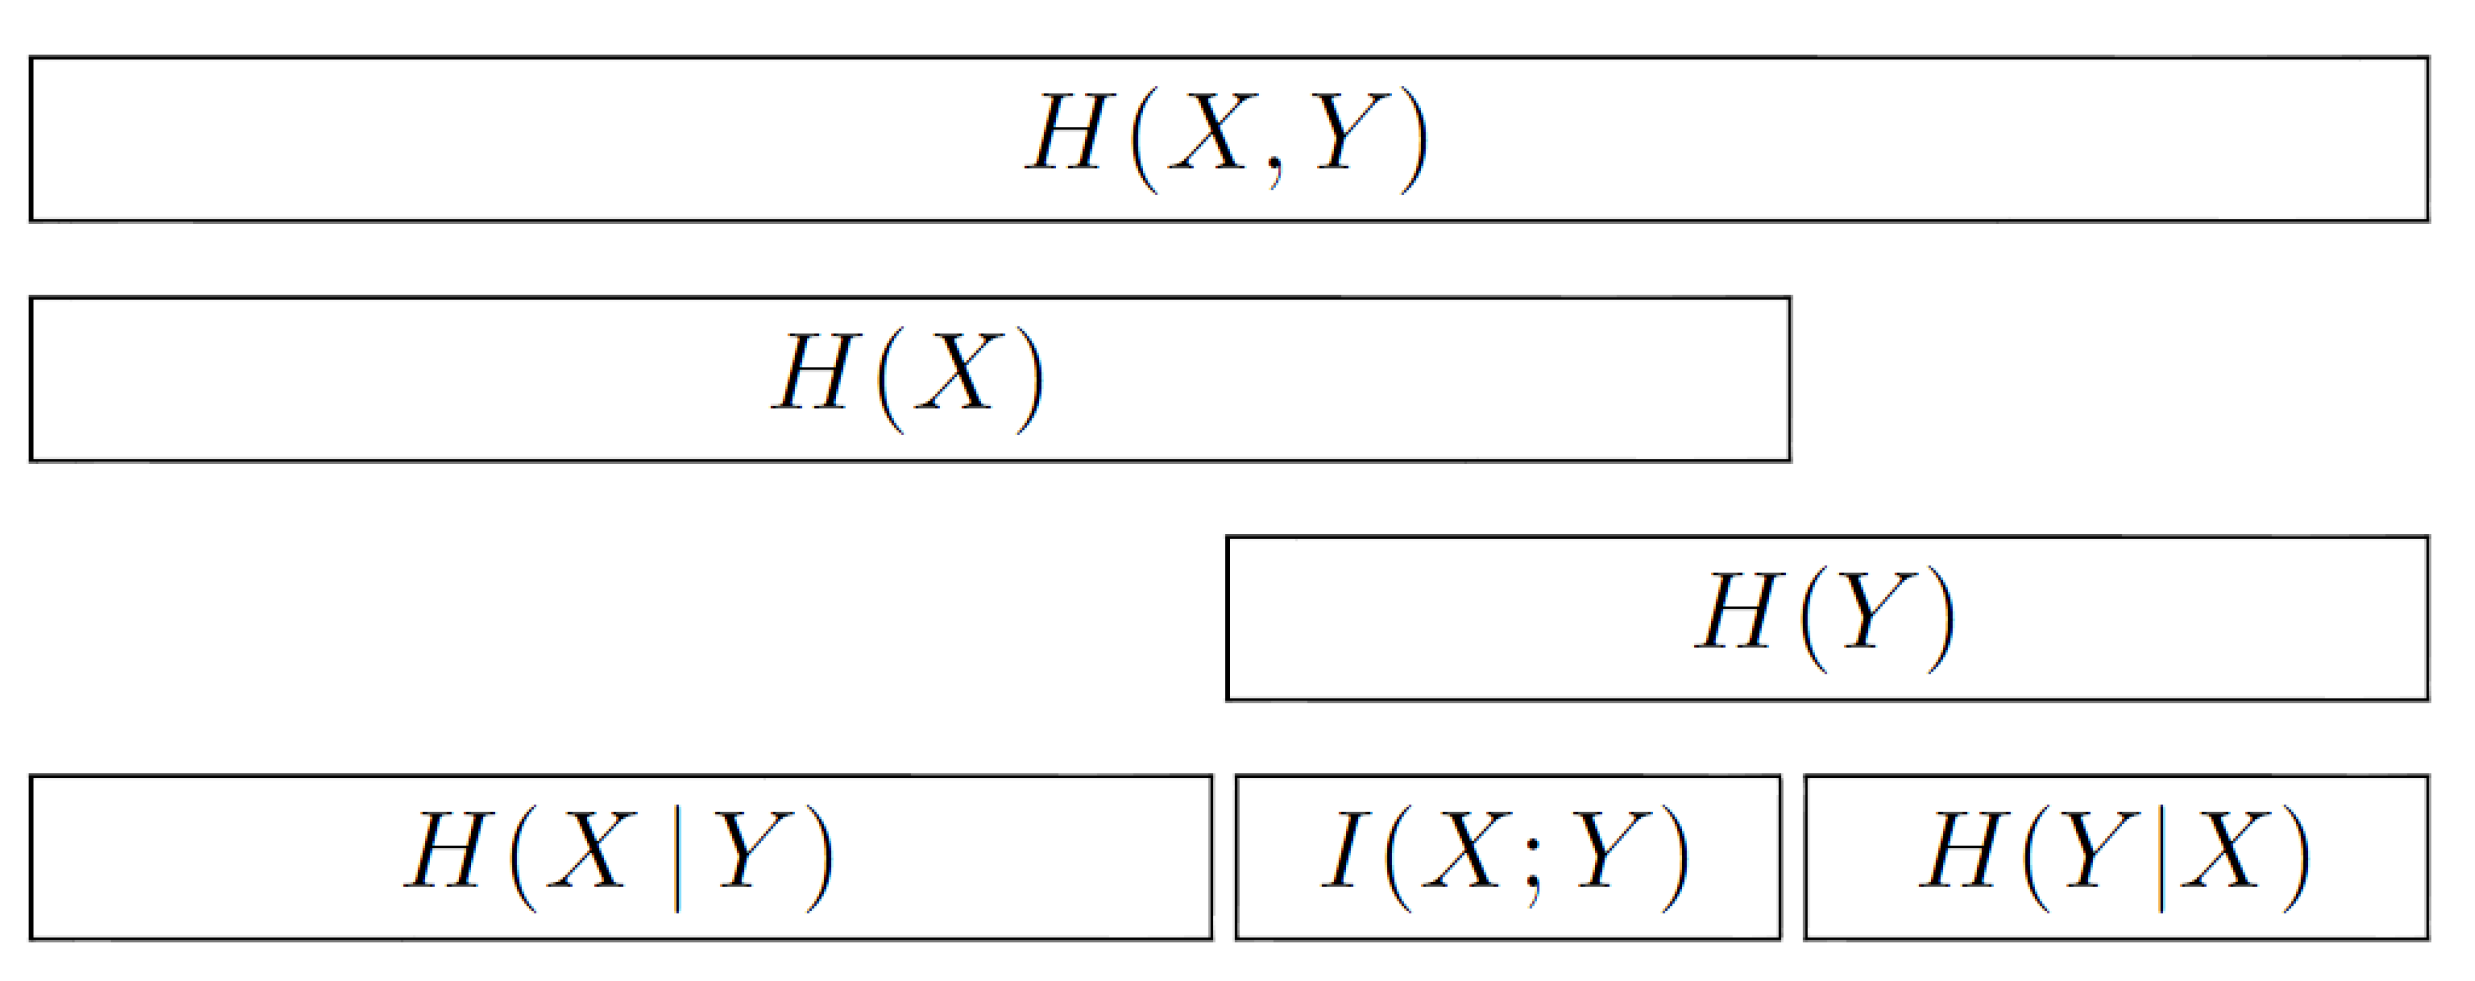
\includegraphics[width=.9\textwidth]{../fig/transinfo.png}
\end{center}

\section{Kanalkapazität}
Die Kapazität eines Kanals entspricht der maximalen Transinformation des Kanals 
bei Speisung mit einer angepassten Quelle [bit/Kanalnutzung]:
\[ C = \max_X I(X;Y) \]
~\\
Bei symmetrischen diskreten gedächtnislosen Kanälen wird die Kanalkapazität 
durch eine Quelle mit Gleichverteilung erreicht. 
\\\\
kontinuierliche AWGN-Kanäle [bit/s]:
\[ C_{AWGN} = B\log_2\left(1+\frac{\bar{P}}{N_0 \cdot B}\right) \]
~\\
\begin{footnotesize}
\begin{tabular}{ll}
	$B$:	& Bandbreite \\
	$\bar{P}$:	& mittlere empfangene Signalleistung \\
	$N_0$:&	spektr. Rauschleistungsdichte
\end{tabular}
\end{footnotesize}

\chapter{Kanalcodierung}
\begin{center}
	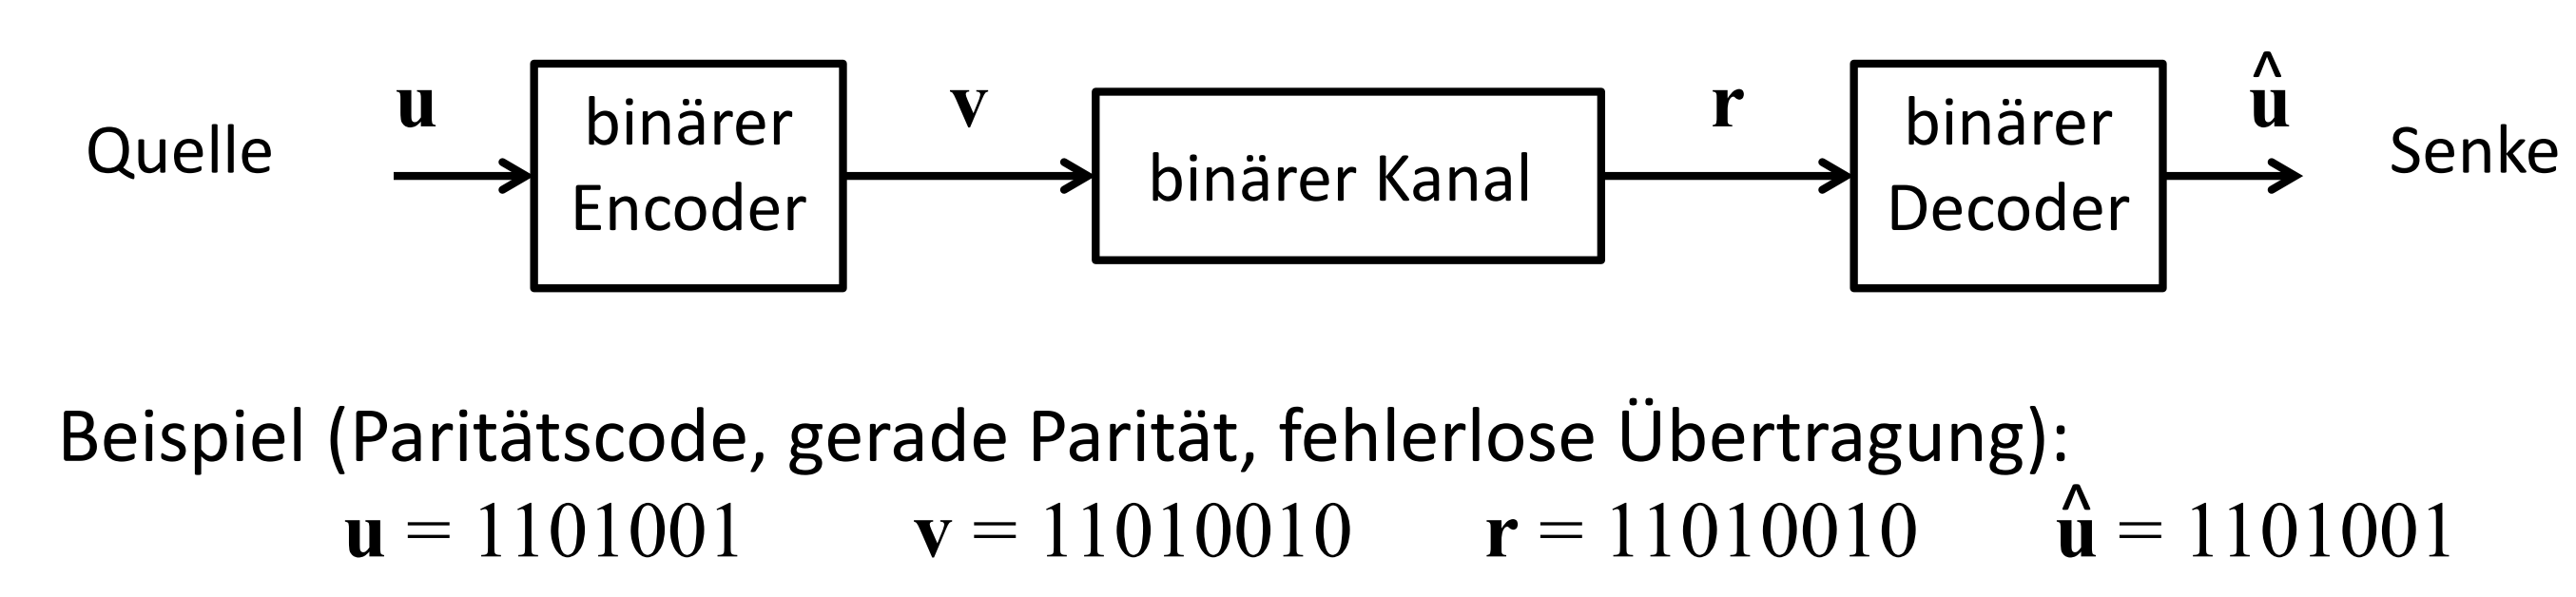
\includegraphics[width=.9\textwidth]{../fig/bincode.png}
\end{center}
\section{Paritätscode}
Nachricht:
\[ \textbf{u} = \underbrace{
	\begin{bmatrix}1 & 1 & 0 & 1 & 0 & 0 & 1\end{bmatrix}
	}_\textrm{$k$ bits} \]
~\\
Codewort:
\[ \textbf{v} = \underbrace{
	\begin{bmatrix}1 & 1 & 0 & 1 & 0 & 0 & 1 & 0\end{bmatrix}
	}_\textrm{$n$ bits} \]
~\\
Coderate:
\[ R = \frac{k}{n} \]
\section{Repetitionscode}
Jedes Bit wird $N$-mal wiederholt, somit ist die Coderate $\frac{1}{N}$.

\section{Generatormatrix}
Nachricht \textbf{u}: Zeilenvektor der Länge $k$\\
Codewort \textbf{v}: Zeilenvektor der Länge $n$\\
Generatormatrix \textbf{G}: ($k\times n$)-Matrix\\
\[ \textbf{v} = \textbf{u} \cdot \textbf{G} \]
~\\
Hamming Code (7,4):
\[ G_{n=7,k=4} = \begin{bmatrix}
	1 & 0 & 0 & 0 & 1 & 0 & 1 \\
	0 & 1 & 0 & 0 & 1 & 1 & 0 \\
	0 & 0 & 1 & 0 & 1 & 1 & 1 \\
	0 & 0 & 0 & 1 & 0 & 1 & 1 \\
\end{bmatrix} \]
~\\
\textbf{Linearität}: Zur Berechnung z.B. der minimalen Hamming-Distanz des Codes darf wegen 
der Linearität stets das Codewort  \textbf{v = 0} als Referenz genommen werden.
\\\\
Aufbau:
\[ \textbf{G} = \left[\textbf{I}_k|\textbf{P}_{k\times (n-k)}\right] \]
~\\
Party-check Matrix:
\[ \textbf{H} = \left[\textbf{P}^T | \textbf{I}_{n-k}\right] \]
~\\
Empfangener Symbolvektor:
\[ \textbf{r} = \textbf{u} \cdot \textbf{G} + \textbf{n} \]
~\\
Syndrom:
\[ \textbf{s} = \textbf{r} \cdot \textbf{H}^T = \textbf{n} \cdot \textbf{H}^T \]

\section{Optimale Decodierung}
AWGN Kanal mit bin. Eingang:
\[ p(r_i|V_i=1) = \frac{1}{\sqrt{2\pi\sigma^2}} \e^{-\frac{(r_i-1)^2}{2\sigma^2}} \]
\[ p(r_i|V_i=0) = \frac{1}{\sqrt{2\pi\sigma^2}} \e^{-\frac{(r_i+1)^2}{2\sigma^2}} \]

\begin{center}
	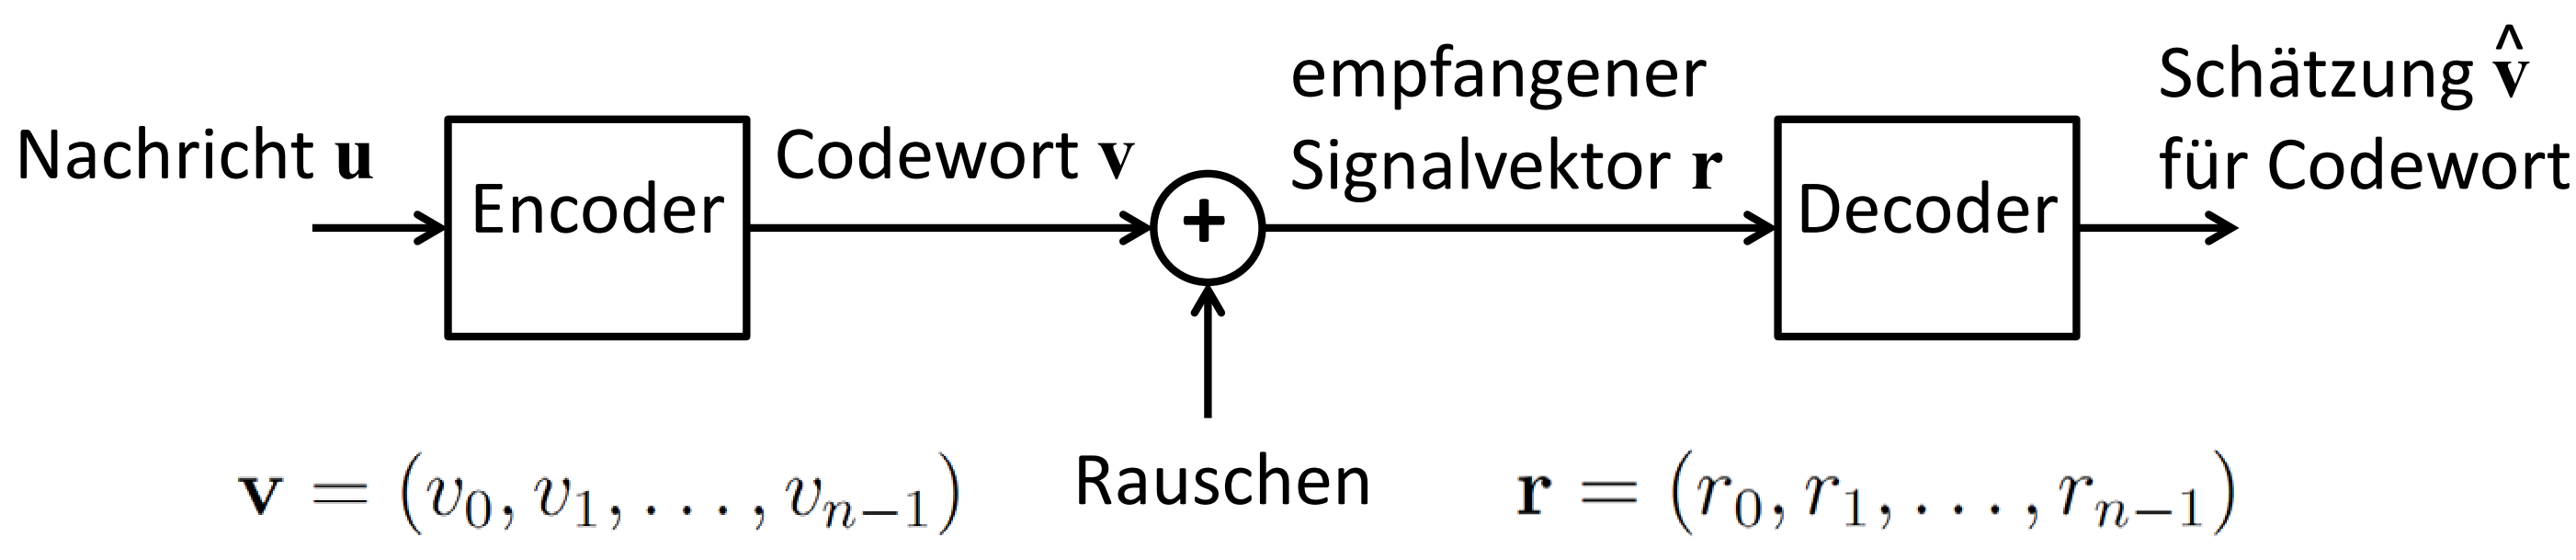
\includegraphics[width=.9\textwidth]{../fig/optdecode.png}
\end{center}
Satz von Bayes:
\[ p(y_j|x_i) = \frac{p(y_j) \cdot p(x_i|y_j)}{p(x_i)} \]
Maximum a posteriori Schätung:
\[ \hat{\textbf{v}} = \arg\max p(\textbf{v}|\textbf{r}) \]
~\\
Maximum-Likelihood Decodierung:
\[ \hat{\textbf{v}} = \arg\max p(\textbf{r}|\textbf{v}) =
	\arg\max\log p(\textbf{r}|\textbf{v}) \]
~\\
Log-likelihood-Funktion:
\[ \log p(\textbf{r}|\textbf{v}) = \sum_{i=0}^{n-1} \log p(r_i|v_i) \]
~\\
Liklihood-Verhältnis:
\[ \frac{p(r_i|V_i=1)}{r_i|V_i=0} \]
~\\
Log-Liklihood ratio:
\[ \Lambda(r_i) = \log\frac{p(r_i|V_i=1)}{r_i|V_i=0} \]
\[ \Lambda(r_i) = \frac{2r_i}{\sigma^2} \qquad \textrm{für bin AWGN Kanal}\]
~\\
Branch-Metrik:
\[ L_i(v_i) = \left\lbrace \begin{matrix}
		\Lambda(r_i)  & \textrm{für } v_i=1\\
		-\Lambda(r_i) & \textrm{für } v_i=0\\
	\end{matrix} \right. \]
~\\
Pfadmetrik:
\[ L(\textbf{v}) = \sum_{i=0}^{n-1}L_i(v_i) \]

\section{Faltungscodes}
($n,k,m$)-Faltungscode:
\begin{itemize}
	\item $n$: Anzahl Ausgangsbits pro Takt
	\item $k$: Anzahl Eingangsbits pro Takt
	\item $m$: Anzahl innere Speicher
\end{itemize}
~\\
Rate: $\frac{k}{n}$

\begin{center}
	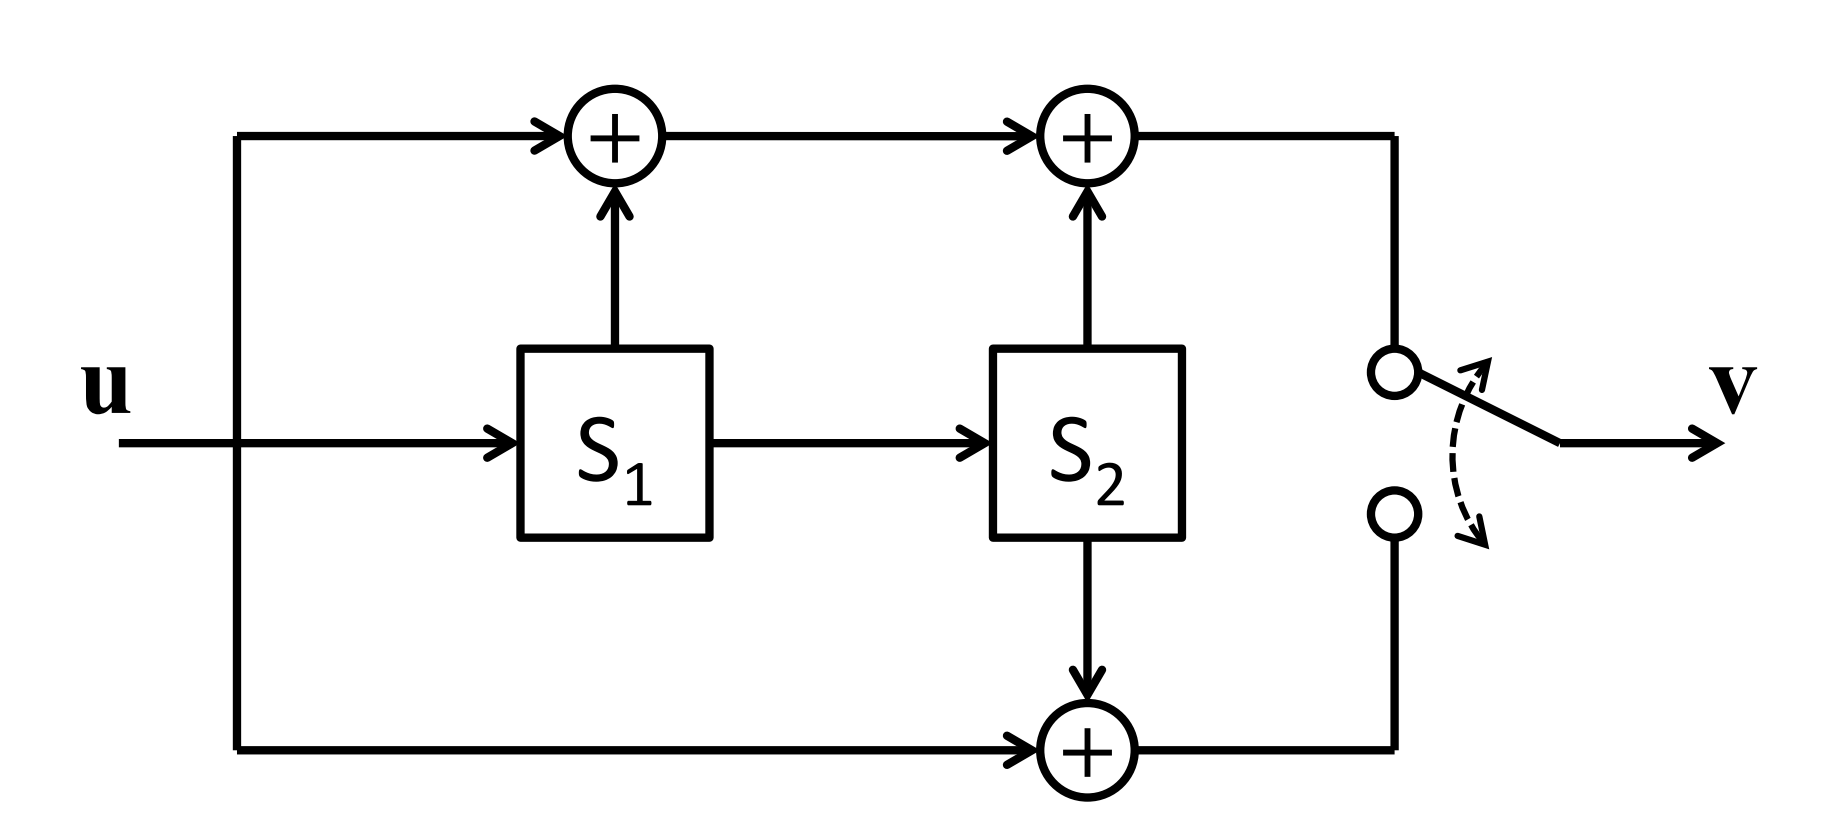
\includegraphics[width=.9\textwidth]{../fig/faltungscode.png}
\end{center}

\begin{center}
	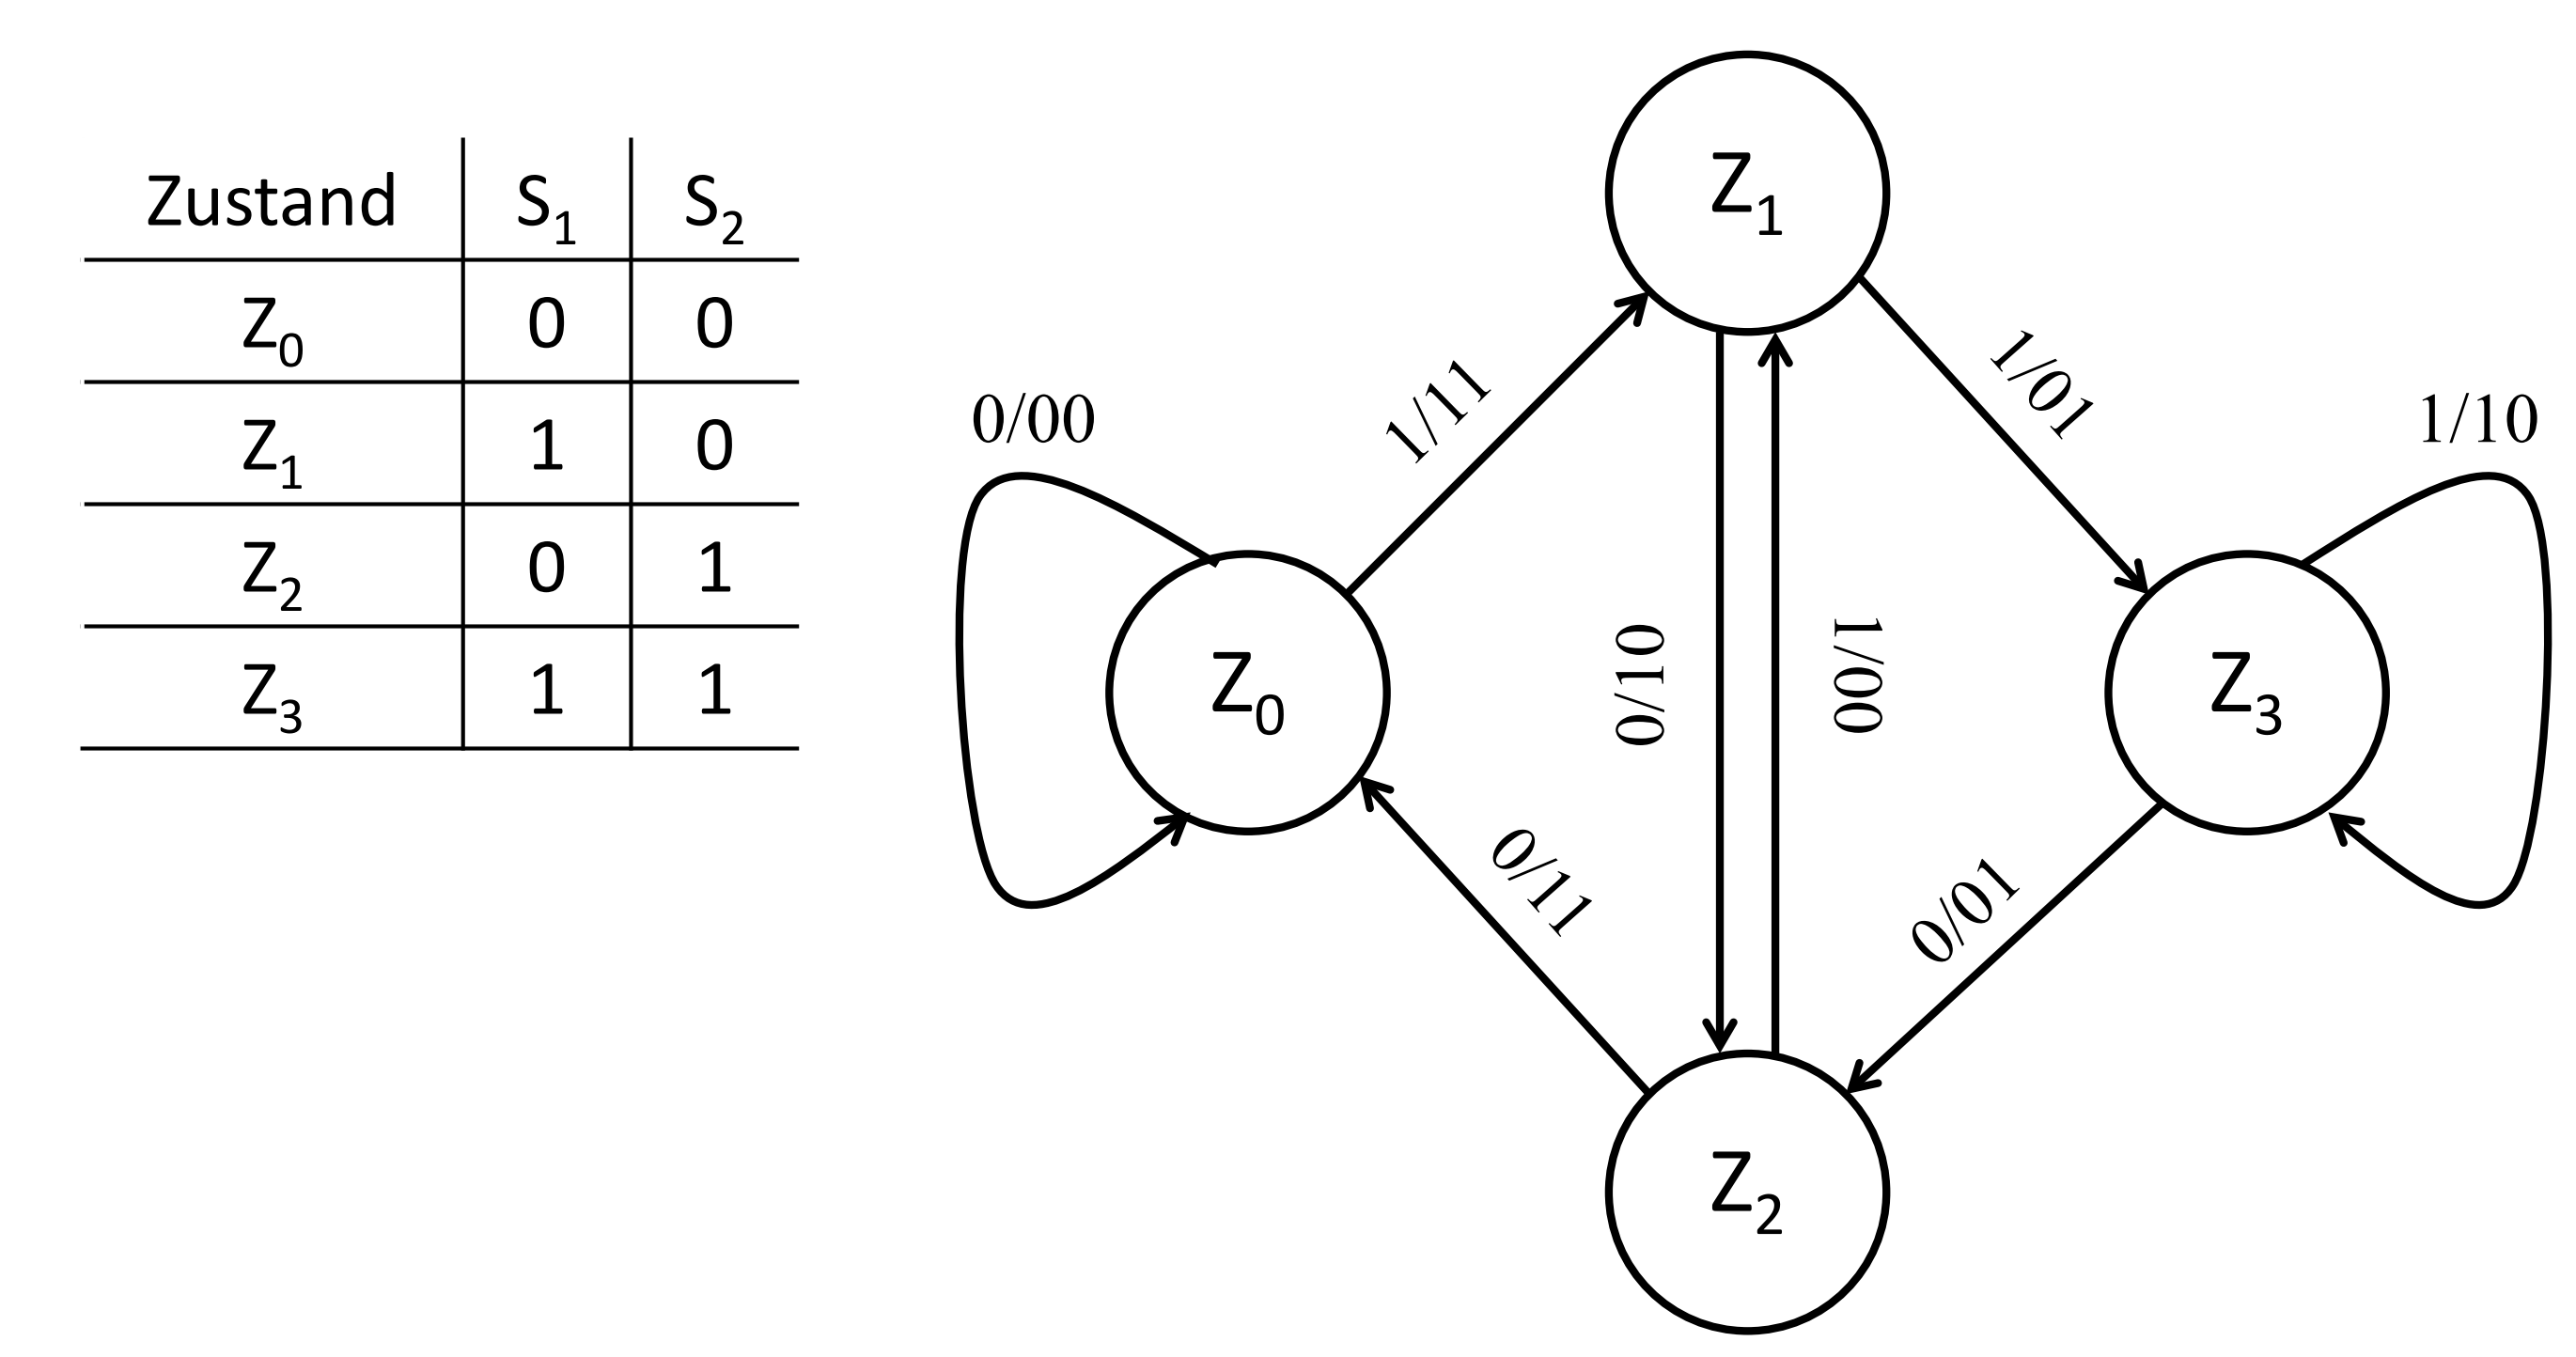
\includegraphics[width=.9\textwidth]{../fig/zustand.png}
\end{center}


\end{document}

